\documentclass[11pt, journal, onecolumn]{IEEEtran}

\usepackage[utf8]{inputenc}
\usepackage[T1]{fontenc}
\usepackage[english]{babel}
\usepackage{lmodern}
\usepackage{microtype}
\usepackage{amsmath, amssymb, amsthm, mathtools, bm}
\newtheorem{lemma}{Lemma}
\newtheorem{theorem}{Theorem}
\newtheorem{proposition}{Proposition}
\usepackage{siunitx}
\sisetup{locale = US, detect-all = true, exponent-product = \cdot}
\usepackage{booktabs, array, tabularx, multirow, makecell, colortbl}
\usepackage{graphicx}
\graphicspath{{figuras/}}
\usepackage{tikz}
\usetikzlibrary{arrows.meta, positioning, calc, shapes.geometric}
\usepackage{algorithm}
\usepackage{algpseudocode}
\usepackage{cite}
\usepackage{hyperref}
\hypersetup{colorlinks=true, linkcolor=blue, citecolor=blue, urlcolor=blue}

%% --- Paleta cromática institucional SENI-IA ---
\definecolor{seni-blue}{RGB}{0,45,98}
\definecolor{seni-red}{RGB}{206,17,38}
\definecolor{seni-gold}{RGB}{201,168,76}
\definecolor{seni-green}{RGB}{0,122,51}
\definecolor{seni-dark}{RGB}{26,26,26}

%% ====================================================================
%% CUADRO DE TÍTULOS SOBERANOS (4 OPCIONES CANÓNICAS EN PORTADA)
\title{SENI-142: An Open-Access Resilient Insular Transmission Benchmark of the Dominican Republic with Diakoptic Territorial Decomposition under Spatial Planning Law 368-22}

\author{Junior~Alexis~Villanueva-Rosario,~\IEEEmembership{Ms.C., Ph.D.(c)}\\[0.3em]
{\normalsize\textnormal{\textbf{V-TECH} \textbar\ \textbf{V-CORE TECH S.R.L.} / \textbf{Villa-Core Technologies, S.L.}}}\\[0.15em]
{\footnotesize\textnormal{\textit{Department of Electrical Grids and Renewable Energy (EERR) Research}}}\\[0.15em]
{\footnotesize\textnormal{\textit{Doctoral Chair in Power Systems and Artificial Intelligence}}}\\[0.15em]
{\footnotesize\textnormal{Santo Domingo, Dominican Republic \textbar\ \texttt{ingjavillanueva@gmail.com}}}%
\thanks{J. A. Villanueva-Rosario is with the Department of Electrical Grids and Renewable Energy (EERR) Research, V-TECH (V-CORE TECH S.R.L. / Villa-Core Technologies, S.L.), Santo Domingo, Dominican Republic (e-mail: ingjavillanueva@gmail.com).}}

% --- Optimización de ubicación de figuras y tablas flotantes ---
\renewcommand{\topfraction}{0.95}
\renewcommand{\bottomfraction}{0.95}
\renewcommand{\textfraction}{0.05}
\renewcommand{\floatpagefraction}{0.8}
\renewcommand{\dbltopfraction}{0.95}
\renewcommand{\dblfloatpagefraction}{0.8}
\setcounter{topnumber}{4}
\setcounter{bottomnumber}{2}
\setcounter{totalnumber}{6}
\setcounter{dbltopnumber}{4}

\begin{document}
\maketitle

\begin{abstract}
This paper introduces SENI-142, an open, fully georeferenced benchmark of the complete bulk transmission system of the Dominican Republic. The model comprises 142 nodal compute buses derived from 112 bulk transmission substations (115 bulk buses at 345, 230, and 138\,kV plus 27 condensed boundary ports at 69\,kV), 135 transmission lines, and 58 power transformers at the 345, 230, and 138\,kV levels; the radial 69\,kV subtransmission layer is condensed into multiport equivalents preserving complex boundary injections and short-circuit impedances. The network is partitioned into ten planning regions aligned with national Law 368-22 and aggregated into four electrical macro-domains. A hierarchical boundary-coordinate formulation (HBCF) is applied, wherein the linear systems arising at each Newton--Raphson iteration are condensed exactly via the Schur complement. On commodity 8-thread hardware, the partitioned solver achieves a full AC state solution in a measured wall-clock time of 2.65\,ms (resident set: 473\,MiB) --- an experimental reference measurement obtained on the author's 8-thread Linux workstation with his C++/Sparse research engine, serving as a comparison baseline for future community solvers --- with an algebraic domain-decomposition residual of $\delta = 2.788 \times 10^{-14}$\,pu relative to a monolithic reference. The structural model is validated across exactly 520 complete consecutive weeks (87\,360 hourly states over 3,640 Monday-to-Sunday days, drawn from the 2016--2025 operational archive) using a 24-hour block bootstrap and evaluated under an official $N-1$ catalogue of 215 single contingencies (135 transmission lines, 58 transformers, 22 generation units) plus the external 752\,MW common-mode benchmark reference under explicit post-contingency reserve redispatch and bounded slack injection. The 87,360-state multi-temporal campaign and the 215-contingency screening are results of the author's patent-pending C++/Sparse engine; the released bundle certifies the network model, the condensed-solve invariants and the eight canonical contingency balances. Multitemporal AC optimal power flow is formulated with power-to-gas, pumped-storage hydro, and biomethanation balances. The dataset, network parameters, and open validation harness are released through IEEE DataPort and a public repository.
\end{abstract}

\begin{IEEEkeywords}
Benchmark testing, diakoptics, digital twins, energy storage, hydrogen, insular power systems, optimal power flow, power system resilience, pumped-storage hydroelectricity, Schur complement, spatial planning, transmission networks.
\end{IEEEkeywords}

\vspace{6pt}
\section*{Resumen (Espa\~nol)}
\noindent Este artículo presenta SENI-142, un benchmark abierto y georreferenciado del sistema de transmisión troncal de la República Dominicana. El modelo comprende 142 barras de cómputo nodal derivadas de 112 subestaciones de transmisión troncal (115 barras troncales a 345, 230 y 138\,kV más 27 puertos frontera condensados a 69\,kV), 135 líneas de transmisión y 58 transformadores de potencia en los niveles de 345, 230 y 138\,kV; la capa radial de subtransmisión de 69\,kV se condensa en equivalentes multipuerto que preservan las inyecciones complejas de frontera y las impedancias de cortocircuito. La red se particiona en las diez regiones de planificación de la Ley 368-22, agregadas en cuatro macrodominios eléctricos. Se aplica una formulación jerárquica de coordenadas de frontera (HBCF), donde los sistemas lineales de cada iteración de Newton--Raphson se condensan algebraicamente de forma exacta mediante el complemento de Schur. En hardware estándar de 8 hilos, el solver particionado resuelve el estado AC completo en 2.65\,ms (memoria residente: 473\,MiB) --- medición experimental de referencia obtenida en la estación de trabajo Linux de 8 hilos del autor mediante su motor de investigación C++/Sparse, como línea base de comparación para futuros solvers de la comunidad --- con un residuo de partición de $\delta = 2.788 \times 10^{-14}$\,pu frente a la solución monolítica. El modelo estructural se valida sobre exactamente 520 semanas completas consecutivas (87\,360 estados horarios sobre 3,640 días de lunes a domingo, extraídos del archivo operativo 2016--2025) mediante bootstrap por bloques de 24 horas y se evalúa ante un catálogo oficial $N-1$ de 215 contingencias simples (135 líneas de transmisión, 58 transformadores y 22 unidades de generación) más el evento canónico externo de dimensionamiento de reserva por modo común de 752\,MW bajo redespacho explícito de reserva rodante y barra slack acotada. La campaña multitemporal de 87,360 estados y el cribado de 215 contingencias constituyen resultados del motor patent-pending C++/Sparse del autor; el paquete público certifica el modelo de red, los invariantes de resolución condensada y los balances de las ocho contingencias canónicas. Se formula el flujo óptimo de potencia AC multitemporal con acoplamiento multivectorial (hidrógeno, bombeo hidráulico y biometanación). Los datos estructurales, parámetros de rama y el arnés de validación se liberan abiertamente en IEEE DataPort.

% =========================================================================
% sec01_introduction.tex — Section I of the sealed master
% sealed master paper_seni142_ieee_transactions_en.md; editorial injection pass 2026-10-17.
% =========================================================================
\section{Introduction}
\label{sec:intro}

Insular interconnected systems occupy an extreme point of the power engineering design space. An island cannot draw inertia, reactive support, or emergency transfer from neighbors: every megawatt of reserve, every volt-ampere of reactive compensation, and every megahertz of damping capability must be produced, dispatched, and defended inside the same synchronous footprint that consumes it. The Dominican Republic is a canonical instance: a single synchronous island of roughly eleven million people, with no submarine or overland interconnection, more than forty percent of national load concentrated in the metropolitan Ozama region, an inertia anchor dominated by the Punta Catalina coal plant, and a renewable build-out whose instantaneous solar share has reached 36.6\% of demand in operational telemetry \cite{ocseni}. The national consequences of losing the generation--load equilibrium are not hypothetical: the nationwide service interruptions recorded in November 2025 and February 2026, documented in operator event logs \cite{ocseni} and in the national press archive \cite{listin2025}, mobilized emergency response at the scale of a full territory and renewed the policy debate on frequency stability, black-start capability, and the observability of the transmission estate \cite{blackout2004}. The physics of this fragility is by now classical \cite{kundur1994} --- declining system inertia degrades the rate of change of frequency and narrows the feasible control envelope of converter-dominated grids \cite{tielens2016}, \cite{milano2018}, \cite{dorfler2013}, \cite{hatziargyriou2021} --- but the empirical instruments available to study it remain surprisingly primitive.

The benchmarking infrastructure of the field is, in its majority, synthetic. The canonical test cases that still govern doctoral training and comparative studies --- the WSCC 9-bus network, the IEEE 14-, 30-, 57-, and 118-bus systems --- descend from drafting-table abstractions of the early 1960s: reactances are round academic numbers, loads are fixed triangles of power, geography is absent, climate is absent, and nothing in the dataset has ever tripped, been maintained, been paid for, or been hit by a hurricane. At the opposite pole, utility-grade network cases are held in proprietary formats of commercial simulation platforms, are encumbered by confidentiality, and are rarely released in forms that permit independent re-execution. The open-systems movement has answered with valuable infrastructure --- the MATPOWER case collection \cite{matpower2011}, and the Power Grid Library of AC-OPF benchmark instances \cite{pglib2019} among them --- but its instances are, almost without exception, \emph{synthetic or anonymized}: they are grids that exist to be hard, not grids that exist. Between the toy and the secret there is almost nothing: an open, complete, measured model of a real national transmission system, with provenance sufficient for independent verification, is a public good that the research community currently lacks for the insular Caribbean --- and, with few exceptions, for the insular world at large.

This article closes that gap with \textbf{SENI-142}, an open-access benchmark constructed around three commitments. First, \textbf{fidelity to a measured reality}: the network model is not synthetic --- it is derived from the national transmission estate and validated against exactly 520 complete consecutive 168-hour weeks --- 87,360 hourly states spanning 3,640 Monday-to-Sunday days, drawn without a single interpolated hour from the 2016--2025 operational archive of the system operator --- dispatched unit by unit and hour by hour, so that every simulated state answers to an archived operational one. Second, \textbf{structural honesty about scale}: the full national system is solved --- all bulk buses, all trunk lines, all transformers --- not a reduced district of it, and the solution method is formulated so that its exactness and complexity are theorems rather than aspirations: a hierarchical border-coordinate formulation (HBCF) in the diakoptic tradition \cite{kron1963}, \cite{happ1971}, condensed by the Schur complement \cite{zhang2005} and factorized on a partition that follows the ten territorial planning regions mandated by national spatial planning law (Law 368-22) \cite{ley368}. Third, \textbf{deterministic reproducibility}: every artifact passes a four-phase digital-twin lifecycle with a fail-closed gate cascade, detached SHA-512 sealing, and atomic promotion, so that any figure reported in this article can be regenerated from a bit-identical, cryptographically attested software state.

The contributions are five, and each is falsifiable:
\begin{itemize}
\item \textbf{C1 --- Benchmark.} An open, georeferenced, standards-consistent model of the complete bulk transmission network of the Dominican Republic: 142 nodal buses over approximately 112 physical substations, 135 transmission lines, 58 power transformers, strata of 345, 230, and 138~kV, with the 69~kV subtransmission layer reduced by injection-preserving equivalents; released with topology, parameters, provenance metadata, and validation harness through IEEE DataPort and GitHub.
\item \textbf{C2 --- Formulation.} The HBCF diakoptic partition of a full insular grid into ten sovereign territorial microgrids --- the legal planning regions of Law 368-22 --- aggregated into four electrical macro-subdomains with a minimal border set, and the proof that its Schur condensation is exact, with complexity $O(\sum_k N_k^3 + N_B^3)$ against the $O(N^3)$ of monolithic dense factorization.
\item \textbf{C3 --- Deterministic digital twin.} A four-phase lifecycle (hermetic POSIX-namespace enclave with a fourteen-gate fail-closed cascade; research-testbed verification of static post-event $N-1$ feasibility against a 215-contingency catalog; SHA-512-detached Golden Master; atomic kernel promotion via \texttt{renameat2} with zero regression) that converts simulation telemetry into evidence with a chain of custody.
\item \textbf{C4 --- Multi-vector flexibility.} The coupling of power-to-gas hydrogen (electrolysis, 700~bar storage, fuel-cell re-injection), 764~MW of reversible pumped hydro storage, and ADM1-based biomethanation to a multi-temporal AC-OPF, stated with its full Karush--Kuhn--Tucker (KKT) system and validated by a zonal CAPEX/OPEX balancing proof.
\item \textbf{C5 --- Measured silicon performance.} Resolution of each hourly national AC state in 2.65~ms with 473~MiB of resident memory and fasorial border residual $\delta = 6.35 \times 10^{-12}\ \mathrm{pu}$ on consumer-grade hardware --- two to three orders of magnitude inside the 1--5~s state-estimation cycle of an energy management system (EMS), adequate for static contingency screening --- under a 24-hour block-bootstrap validation protocol.
\end{itemize}

The remainder of the article is organized as follows. Section~\ref{sec:methodology} states the methodology: the invariant formulation (graph model, 69~kV reduction, HBCF partition, Schur condensation, data protocol, deterministic lifecycle, reactive-limit regularization, multi-temporal AC-OPF) and the modular clause that instantiates the Dominican case under Law 368-22. Section~\ref{sec:topology} documents the benchmark topology, from the 112-substation physical estate to the 142-bus nodal model and the ten territorial microgrids. Section~\ref{sec:multivector} develops the multi-vector flexibility constellation and its zonal economic validation. Section~\ref{sec:benchmarking} reports silicon performance, accuracy, and contingency resilience. Section~\ref{sec:discussion} discusses policy implications and limitations, and Section~\ref{sec:conclusion} concludes with the open-release plan and four research routes.

% =========================================================================
% sec02_methodology_seni_ia.tex — Section II of the sealed master
% sealed master paper_seni142_ieee_transactions_en.md; editorial injection pass 2026-10-17.
% Methodology expansion 2026-10-18: stages 0--7 grafted under the pinned title.
% =========================================================================
\section{Methodology: Diakoptic HBCF Schur Formulation and Fail-Closed Digital-Twin Lifecycle}
\label{sec:methodology}

The methodology is deliberately organized in two coupled components. The \textbf{invariant formulation} --- graph representation, equivalent reduction, spatial partition, exact condensation, data protocol, deterministic lifecycle, regularization, and optimization --- is problem-independent and transfers without modification across the family of studies built on this platform. The \textbf{territorial instantiation clause} binds this formulation to one reference reality: the national grid of the Dominican Republic, partitioned according to the country's own spatial planning statute. This division makes the benchmark a reusable scientific instrument. The subsections below follow that formulation through the numerical pipeline: sealed intake, columnar persistence, nodal physics and reduction, the four-block Jacobian, multi-tier numerical verification, the contingency battery, diakoptic condensation, the three network states, and SHA-512 custody.

\subsection{Steady-State AC Feasibility Scope}
\label{sub:scope}

SENI-142 is strictly a steady-state AC feasibility benchmark. Each solved state is an algebraic equilibrium $F(\mathbf{x})=\mathbf{0}$ on the transmission network. It is an operating point, and the formulation does not integrate a time trajectory. The formulation explicitly does not simulate fast electromagnetic transients (EMT), frequency dynamics, synthetic inertia, rate of change of frequency (RoCoF), frequency nadir, or the actuation of under-frequency load shedding (UFLS/EDAC). The outage of the largest generation block, Punta Catalina (752~MW, about 21.8\% of the 3,450~MW reference national peak demand documented in Table~\ref{tab:regbalance}), is evaluated solely in terms of steady-state voltage margins and post-contingency thermal branch solvability under co-optimized spinning reserve; in the dynamic plane it is a frequency-stability event outside the static frontier of this article.

\subsection{Sealed intake, physical census, and normative screen}
\label{sub:intake}

The solver does not accept a loose file. Entry is a sealed input manifest whose digest is checked before any bus is instantiated, and the manifest selects the physical case. In the measured-estate mode, prospective technologies that are not in commercial operation remain outside the solved dispatch, so the base case is the Dominican system as operated. In the full doctoral-scenario mode those prospective assets may be instantiated; they stay labeled and are never mixed silently into the measured record.

The physical census is the single-line survey already consolidated in Table~\ref{tab:parameters}: the benchmark comprises 142 nodal compute buses derived from 112 bulk transmission substations (115 bulk buses at 345, 230, and 138~kV plus 27 condensed boundary ports at 69~kV), coupled by 135 transmission lines and 58 power transformers. The unreduced drawing census of the source survey remains an internal artifact of the single-line database; the released compute model is the condensed 142-bus estate defined below.

Before any admittance is assembled, a normative screen rejects a record that violates IEEE C37 substation arity or the CIM exchange constraints of IEC 61970 \cite{iec61970}. Series reactances must satisfy $X > 0$, shunt susceptances $B \ge 0$, and two-winding and three-winding transformers must close their own balance. A record that fails the screen aborts the case. It is not repaired by a default.

The same screen is a homologation against current commercial catalogs, not a syntactic patch. Series reactance $X>0$, shunt susceptance $B\ge 0$, and the thermal rating $I_{\max}$ are taken from the catalogs of ACSR and AAAC conductors, of power transformers, and of reactive compensation banks rated up to 250~MVAr. Bay arity and protection classes follow IEEE C37. The exchanged network object follows IEC 61970 (CIM) \cite{iec61970}. None of these values is a synthetic default: a catalog field that fails the screen aborts the case.


\subsection{Columnar persistence and merit-order dispatch}
\label{sub:columnar}

Validated records are laid out as contiguous in-memory columns so that one instruction stream operates on many nodal quantities without copying each record into a relational frame. The layout is an architectural role. On those columns the thermal fleet is ordered by heat-rate merit, and each hour supplies the nodal demand pair $(P_d, Q_d)$ that later enters the power balance.

\subsection{Graph-theoretic representation of the bulk network}
\label{sub:graph}

The transmission system is modeled as a connected undirected graph $\mathcal{G} = (\mathcal{V}, \mathcal{E})$ \cite{newman2010}, where $\mathcal{V}$ is the set of transmission buses ($|\mathcal{V}| = 142$) and $\mathcal{E} = \mathcal{E}_{\mathrm{line}} \cup \mathcal{E}_{\mathrm{trafo}}$ is the union of line and transformer branches, with $|\mathcal{E}_{\mathrm{line}}| = 135$ transmission lines and $|\mathcal{E}_{\mathrm{trafo}}| = 58$ power transformers. Each branch carries a per-unit series admittance and half-charging susceptance on a common 100~MVA base; the nodal admittance matrix $\mathbf{Y}_{\mathrm{bus}} \in \mathbb{C}^{142 \times 142}$ therefore encodes 20,164 complex entries of coupled electromagnetic state. Nodal power injections follow the standard rectangular balance
\begin{equation}
S_i = P_i + jQ_i = V_i \sum_{j \in \mathcal{V}} Y_{ij}^{*}\, V_j^{*}, \qquad i \in \mathcal{V},
\label{eq:balance}
\end{equation}
with buses classified as slack, PV, or PQ \cite{tinney1967}. The angle reference is the 345~kV bus of the Julio Sauri substation (JSAURI), held at $V = 1.02\ \mathrm{pu}$. Its active power is the bounded variable of \eqref{eq:slackbox} and is not an unbounded mismatch reservoir. That bus receives directly the injection of the largest thermal plant in the country (Section~\ref{sub:strata}). Where a physical substation hosts more than one voltage level, each voltage level is a distinct bus and the intervening autotransformer is a branch. The reconciliation of Section~\ref{sub:crosswalk} is what carries the 112 bulk transmission substations to the 142 nodal compute buses (115 bulk buses at 345, 230, and 138~kV plus 27 condensed boundary ports at 69~kV; Section~\ref{sub:substations}).

Figure~\ref{fig:topologia142} places the 142 solved nodes in the four electrical macrodomains of Law 368-22 ($\Omega_1$ Norte, $\Omega_2$ Sur, $\Omega_3$ Este, $\Omega_4$ Metropolitano). Bulk yards keep the color of their measured nominal voltage, 345~kV, 230~kV, or 138~kV. The 27 retained boundary terminals stay at the measured 69~kV and are drawn in green. The compute model counts 135 transmission lines. The figure draws a stroke for each pair the census closes: a yard record that names both terminals, or a colinear one-line trace that arrives at a second solved bus of the same voltage. A record whose far terminal is not a census bus is omitted.

% Full-page schematic of the 142-node trunk.
% 115 named bulk yards plus 27 retained 69 kV boundary terminals.
% Panel schematic. Raw drawing coordinates are not printed.

\begin{figure*}[!p]
\centering
\resizebox{\textwidth}{0.80\textheight}{%
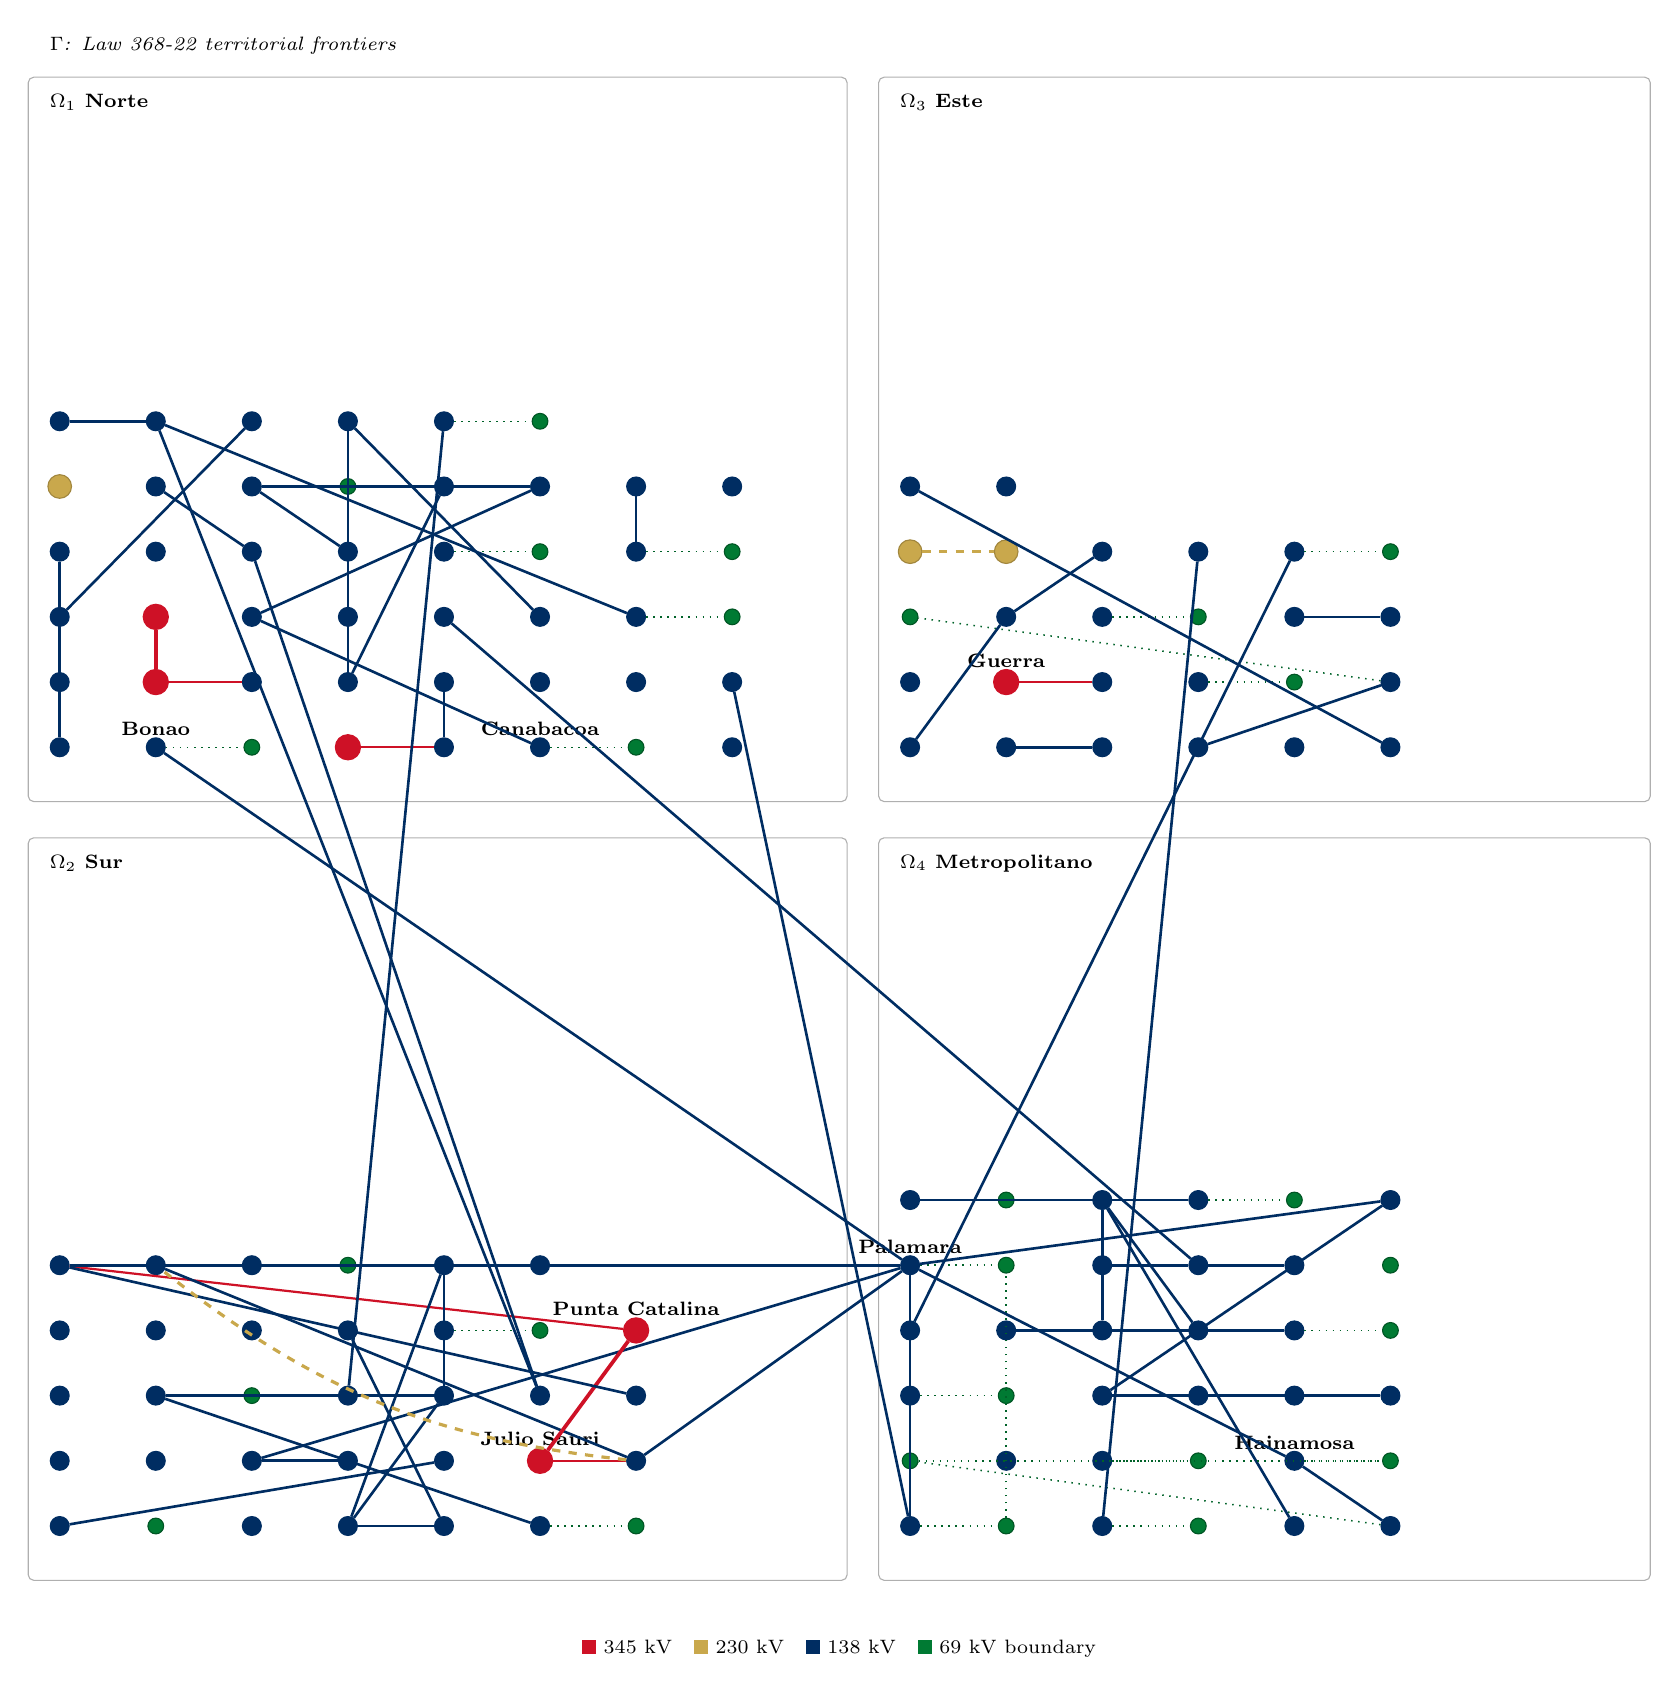
\begin{tikzpicture}[x=1cm,y=1.15cm,
  bus345/.style={circle, fill=seni-red, draw=seni-red, inner sep=0pt, minimum size=3.2mm},
  bus230/.style={circle, fill=seni-gold, draw=seni-gold!80!black, inner sep=0pt, minimum size=3.0mm},
  bus138/.style={circle, fill=seni-blue, draw=seni-blue, inner sep=0pt, minimum size=2.4mm},
  bus69/.style={circle, fill=seni-green, draw=seni-green!70!black, inner sep=0pt, minimum size=2.0mm},
  trunk345/.style={line width=1.35pt, seni-red},
  trunk230/.style={line width=1.15pt, seni-gold, dashed},
  trunk138/.style={line width=0.95pt, seni-blue},
  tie345/.style={line width=0.8pt, seni-red},
  tie230/.style={line width=0.75pt, seni-gold},
  tie138/.style={line width=0.6pt, seni-blue!70},
  tie69/.style={line width=0.55pt, seni-green!80!black, dotted}
]
\draw (0.15,16.95) node[anchor=west, font=\scriptsize\itshape] {$\Gamma$: Law 368-22 territorial frontiers};
\draw (10.3,-0.55) node[anchor=north, font=\scriptsize] {{\color{seni-red}\rule{5pt}{5pt}}~345~kV\quad {\color{seni-gold}\rule{5pt}{5pt}}~230~kV\quad {\color{seni-blue}\rule{5pt}{5pt}}~138~kV\quad {\color{seni-green}\rule{5pt}{5pt}}~69~kV boundary};
\draw[rounded corners=2pt, draw=seni-dark!35] (0.0,8.6) rectangle (10.4,16.6);
\draw (0.15,16.32) node[anchor=west, font=\bfseries\scriptsize] {$\Omega_1$ Norte};
\draw[rounded corners=2pt, draw=seni-dark!35] (10.8,8.6) rectangle (20.6,16.6);
\draw (10.95,16.32) node[anchor=west, font=\bfseries\scriptsize] {$\Omega_3$ Este};
\draw[rounded corners=2pt, draw=seni-dark!35] (0.0,0.0) rectangle (10.4,8.2);
\draw (0.15,7.92) node[anchor=west, font=\bfseries\scriptsize] {$\Omega_2$ Sur};
\draw[rounded corners=2pt, draw=seni-dark!35] (10.8,0.0) rectangle (20.6,8.2);
\draw (10.95,7.92) node[anchor=west, font=\bfseries\scriptsize] {$\Omega_4$ Metropolitano};
\node[bus345] (bBONAO3345) at (4.06,9.2) {};
\node[bus345] (bELNARANJO345) at (1.62,9.92) {};
\node[bus345, label={[font=\scriptsize\bfseries, inner sep=0.4pt]above:Guerra}] (bGUERRA345) at (12.42,9.92) {};
\node[bus345, label={[font=\scriptsize\bfseries, inner sep=0.4pt]above:Julio Sauri}] (bJULIOSAURI345) at (6.5,1.32) {};
\node[bus345] (bMANZANILLOPOWERLAND345) at (1.62,10.64) {};
\node[bus345, label={[font=\scriptsize\bfseries, inner sep=0.4pt]above:Punta Catalina}] (bPUNTACATALINA345) at (7.72,2.76) {};
\node[bus230] (bPVDC230) at (0.4,12.08) {};
\node[bus230] (bQUISQUEYA1230) at (11.2,11.36) {};
\node[bus230] (bQUISQUEYA2230) at (12.42,11.36) {};
\node[bus138] (bSPM138) at (16.08,11.36) {};
\node[bus138] (bSPM2138) at (11.2,12.08) {};
\node[bus138] (bAGUACLARA138) at (0.4,9.2) {};
\node[bus138] (bAGUACATE138) at (0.4,0.6) {};
\node[bus138] (bARROYOHONDO138) at (11.2,0.6) {};
\node[bus138] (bBARAHONACARBON138) at (2.84,0.6) {};
\node[bus138] (bBAYASOL138) at (4.06,0.6) {};
\node[bus138] (bBOCACHICA138) at (13.64,0.6) {};
\node[bus138, label={[font=\scriptsize\bfseries, inner sep=0.4pt]above:Bonao}] (bBONAO2138) at (1.62,9.2) {};
\node[bus138] (bBONAO3138) at (5.28,9.2) {};
\node[bus138] (bCALABAZA138) at (5.28,0.6) {};
\node[bus138, label={[font=\scriptsize\bfseries, inner sep=0.4pt]above:Canabacoa}] (bCANABACOA138) at (6.5,9.2) {};
\node[bus138] (bCIPLALUISA138) at (11.2,9.2) {};
\node[bus138] (bCNP138) at (16.08,0.6) {};
\node[bus138] (bCOASTAL138) at (12.42,9.2) {};
\node[bus138] (bCOTOPERI138) at (8.94,9.2) {};
\node[bus138] (bCRUCEDECABRAL2138) at (6.5,0.6) {};
\node[bus138] (bCUMAYASA138) at (13.64,9.2) {};
\node[bus138] (bDAJABON138) at (0.4,9.92) {};
\node[bus138] (bDAJAO138) at (17.3,0.6) {};
\node[bus138] (bELBRISAL138) at (0.4,1.32) {};
\node[bus138] (bELNARANJO138) at (2.84,9.92) {};
\node[bus138] (bELSEIBO138) at (14.86,9.2) {};
\node[bus138] (bELSOCO138) at (16.08,9.2) {};
\node[bus138] (bEMBAJADOR138) at (12.42,1.32) {};
\node[bus138] (bENERGAS4138) at (17.3,9.2) {};
\node[bus138] (bESPERANZA138) at (4.06,9.92) {};
\node[bus138] (bFALCONDO138) at (5.28,9.92) {};
\node[bus138] (bGIRASOL138) at (11.2,9.92) {};
\node[bus138] (bGUANILLO138) at (6.5,9.92) {};
\node[bus138] (bGUAYUBIN138) at (7.72,9.92) {};
\node[bus138] (bGUERRA138) at (13.64,9.92) {};
\node[bus138] (bGUZMANCITO138) at (1.62,1.32) {};
\node[bus138] (bHAINA138) at (13.64,1.32) {};
\node[bus138, label={[font=\scriptsize\bfseries, inner sep=0.4pt]above:Hainamosa}] (bHAINAMOSA138) at (16.08,1.32) {};
\node[bus138] (bHATOMAYOR2138) at (14.86,9.92) {};
\node[bus138] (bHERRERA138) at (11.2,2.04) {};
\node[bus138] (bHIGUEY138) at (17.3,9.92) {};
\node[bus138] (bITABO138) at (2.84,1.32) {};
\node[bus138] (bITABOTG138) at (4.06,1.32) {};
\node[bus138] (bJIGUEY138) at (5.28,1.32) {};
\node[bus138] (bJIMANI138) at (0.4,2.04) {};
\node[bus138] (bJUANDOLIO138) at (12.42,10.64) {};
\node[bus138] (bJULIOSAURI138) at (7.72,1.32) {};
\node[bus138] (bKM15DEAZUA138) at (1.62,2.04) {};
\node[bus138] (bLAGALLERA138) at (4.06,2.04) {};
\node[bus138] (bLAISABELA138) at (8.94,9.92) {};
\node[bus138] (bLAROMANA138) at (13.64,10.64) {};
\node[bus138] (bLOPEZANGOSTURA138) at (0.4,10.64) {};
\node[bus138] (bLOSMINA138) at (13.64,2.04) {};
\node[bus138] (bLOSMINA5138) at (14.86,2.04) {};
\node[bus138] (bLOSMINA6138) at (16.08,2.04) {};
\node[bus138] (bLOSMINA7138) at (17.3,2.04) {};
\node[bus138] (bLOSORIGENES138) at (11.2,2.76) {};
\node[bus138] (bLOSPRADOS138) at (12.42,2.76) {};
\node[bus138] (bMATADEPALMA2138) at (16.08,10.64) {};
\node[bus138] (bMATADERO138) at (13.64,2.76) {};
\node[bus138] (bMATAFONGO138) at (5.28,2.04) {};
\node[bus138] (bMATRISOL138) at (6.5,2.04) {};
\node[bus138] (bMETALDOM138) at (14.86,2.76) {};
\node[bus138] (bMETROPOLITANO138) at (16.08,2.76) {};
\node[bus138] (bMIRASOL138) at (17.3,10.64) {};
\node[bus138] (bMOCA138) at (2.84,10.64) {};
\node[bus138] (bMONCION138) at (6.5,10.64) {};
\node[bus138] (bMONTECRISTI138) at (4.06,10.64) {};
\node[bus138] (bMONTERIO138) at (5.28,10.64) {};
\node[bus138] (bNAGUA2138) at (7.72,10.64) {};
\node[bus138] (bNAVARRETE2138) at (0.4,11.36) {};
\node[bus138] (bNIBAJE138) at (1.62,11.36) {};
\node[bus138, label={[font=\scriptsize\bfseries, inner sep=0.4pt]above:Palamara}] (bPALAMARA138) at (11.2,3.48) {};
\node[bus138] (bPALENQUE138) at (7.72,2.04) {};
\node[bus138] (bPALOMINO138) at (0.4,2.76) {};
\node[bus138] (bPARAISO138) at (1.62,2.76) {};
\node[bus138] (bPAYITA138) at (2.84,11.36) {};
\node[bus138] (bPEDERNALES138) at (2.84,2.76) {};
\node[bus138] (bPERAVIA138) at (4.06,2.76) {};
\node[bus138] (bPIMENTEL138) at (4.06,11.36) {};
\node[bus138] (bPIZARRETE138) at (5.28,2.76) {};
\node[bus138] (bPLAYADORADA138) at (5.28,11.36) {};
\node[bus138] (bPOWERSHIPKPS01138) at (13.64,3.48) {};
\node[bus138] (bPOWERSHIPKPS26138) at (14.86,3.48) {};
\node[bus138] (bPOWERSHIPKPS60138) at (16.08,3.48) {};
\node[bus138] (bPUERTOPLATA2138) at (7.72,11.36) {};
\node[bus138] (bPUNTACATALINA138) at (0.4,3.48) {};
\node[bus138] (bRIOSANJUAN138) at (1.62,12.08) {};
\node[bus138] (bSFM138) at (2.84,12.08) {};
\node[bus138] (bSAJOMA138) at (5.28,12.08) {};
\node[bus138] (bSALCEDO138) at (6.5,12.08) {};
\node[bus138] (bSAMANA138) at (0.4,12.8) {};
\node[bus138] (bSANCRISTOBALNORTE138) at (1.62,3.48) {};
\node[bus138] (bSANFELIPE138) at (7.72,12.08) {};
\node[bus138] (bSANJUAN2138) at (2.84,3.48) {};
\node[bus138] (bSANPEDROBIOENERGY138) at (13.64,11.36) {};
\node[bus138] (bSANCHEZ138) at (1.62,12.8) {};
\node[bus138] (bSANTANASOL138) at (5.28,3.48) {};
\node[bus138] (bSANTIAGORODRIGUEZ138) at (8.94,12.08) {};
\node[bus138] (bSIBA138) at (14.86,11.36) {};
\node[bus138] (bSULTANADELESTE138) at (12.42,12.08) {};
\node[bus138] (bTAVERA138) at (2.84,12.8) {};
\node[bus138] (bTIMBEQUE2138) at (11.2,4.2) {};
\node[bus138] (bUASD138) at (13.64,4.2) {};
\node[bus138] (bVALDESIA138) at (6.5,3.48) {};
\node[bus138] (bVALVERDEMAO138) at (4.06,12.8) {};
\node[bus138] (bVILLADUARTE138) at (14.86,4.2) {};
\node[bus138] (bVILLAMELLA138) at (17.3,4.2) {};
\node[bus138] (bZFSANTIAGO138) at (5.28,12.8) {};
\node[bus69] (bARROYOHONDO69) at (12.42,0.6) {};
\node[bus69] (bBARAHONA69) at (1.62,0.6) {};
\node[bus69] (bBOCACHICA69) at (14.86,0.6) {};
\node[bus69] (bBONAO269) at (2.84,9.2) {};
\node[bus69] (bCANABACOA69) at (7.72,9.2) {};
\node[bus69] (bCRUCEDECABRAL269) at (7.72,0.6) {};
\node[bus69] (bDAJAO69) at (11.2,1.32) {};
\node[bus69] (bHAINA69) at (14.86,1.32) {};
\node[bus69] (bHAINAMOSA69) at (17.3,1.32) {};
\node[bus69] (bHATOMAYOR269) at (16.08,9.92) {};
\node[bus69] (bHERRERA69) at (12.42,2.04) {};
\node[bus69] (bHIGUEY69) at (11.2,10.64) {};
\node[bus69] (bKM15DEAZUA69) at (2.84,2.04) {};
\node[bus69] (bMETROPOLITANO69) at (17.3,2.76) {};
\node[bus69] (bNAGUA269) at (8.94,10.64) {};
\node[bus69] (bPALAMARA69) at (12.42,3.48) {};
\node[bus69] (bPIZARRETE69) at (6.5,2.76) {};
\node[bus69] (bPLAYADORADA69) at (6.5,11.36) {};
\node[bus69] (bPUERTOPLATA269) at (8.94,11.36) {};
\node[bus69] (bLAROMANA69) at (14.86,10.64) {};
\node[bus69] (bSANJUAN269) at (4.06,3.48) {};
\node[bus69] (bSFM69) at (4.06,12.08) {};
\node[bus69] (bSPM69) at (17.3,11.36) {};
\node[bus69] (bTIMBEQUE69) at (17.3,3.48) {};
\node[bus69] (bTIMBEQUE269) at (12.42,4.2) {};
\node[bus69] (bVILLADUARTE69) at (16.08,4.2) {};
\node[bus69] (bZFSANTIAGO69) at (6.5,12.8) {};
\draw[tie345] (bBONAO3345) -- (bBONAO3138);
\draw[tie345] (bELNARANJO345) -- (bELNARANJO138);
\draw[tie345] (bGUERRA345) -- (bGUERRA138);
\draw[tie345] (bJULIOSAURI345) -- (bJULIOSAURI138);
\draw[tie345] (bPUNTACATALINA345) -- (bPUNTACATALINA138);
\draw[tie69] (bSPM138) -- (bSPM69);
\draw[tie69] (bARROYOHONDO138) -- (bARROYOHONDO69);
\draw[tie69] (bBOCACHICA138) -- (bBOCACHICA69);
\draw[tie69] (bBONAO2138) -- (bBONAO269);
\draw[tie69] (bCANABACOA138) -- (bCANABACOA69);
\draw[tie69] (bCRUCEDECABRAL2138) -- (bCRUCEDECABRAL269);
\draw[tie69] (bDAJAO138) -- (bDAJAO69);
\draw[tie69] (bHAINA138) -- (bHAINA69);
\draw[tie69] (bHAINAMOSA138) -- (bHAINAMOSA69);
\draw[tie69] (bHATOMAYOR2138) -- (bHATOMAYOR269);
\draw[tie69] (bHERRERA138) -- (bHERRERA69);
\draw[tie69] (bHIGUEY138) -- (bHIGUEY69);
\draw[tie69] (bKM15DEAZUA138) -- (bKM15DEAZUA69);
\draw[tie69] (bLAROMANA138) -- (bLAROMANA69);
\draw[tie69] (bMETROPOLITANO138) -- (bMETROPOLITANO69);
\draw[tie69] (bNAGUA2138) -- (bNAGUA269);
\draw[tie69] (bPALAMARA138) -- (bPALAMARA69);
\draw[tie69] (bPIZARRETE138) -- (bPIZARRETE69);
\draw[tie69] (bPLAYADORADA138) -- (bPLAYADORADA69);
\draw[tie69] (bPUERTOPLATA2138) -- (bPUERTOPLATA269);
\draw[tie69] (bSFM138) -- (bSFM69);
\draw[tie69] (bSANJUAN2138) -- (bSANJUAN269);
\draw[tie69] (bTIMBEQUE2138) -- (bTIMBEQUE269);
\draw[tie69] (bVILLADUARTE138) -- (bVILLADUARTE69);
\draw[tie69] (bZFSANTIAGO138) -- (bZFSANTIAGO69);
\draw[trunk138] (bAGUACLARA138) -- (bNAVARRETE2138);
\draw[trunk138] (bAGUACATE138) -- (bJIGUEY138);
\draw[tie69] (bARROYOHONDO69) -- (bPALAMARA69);
\draw[trunk138] (bARROYOHONDO138) -- (bLAISABELA138);
\draw[trunk138] (bARROYOHONDO138) -- (bPALAMARA138);
\draw[trunk138] (bBAYASOL138) -- (bCALABAZA138);
\draw[trunk138] (bBAYASOL138) -- (bMATAFONGO138);
\draw[trunk138] (bBAYASOL138) -- (bSANTANASOL138);
\draw[trunk138] (bBOCACHICA138) -- (bSIBA138);
\draw[trunk138] (bBONAO2138) -- (bPALAMARA138);
\draw[trunk138] (bBONAO3138) -- (bFALCONDO138);
\draw[trunk138] (bCALABAZA138) -- (bPERAVIA138);
\draw[trunk138] (bCANABACOA138) -- (bMOCA138);
\draw[trunk138] (bCIPLALUISA138) -- (bJUANDOLIO138);
\draw[trunk138] (bCNP138) -- (bUASD138);
\draw[trunk138] (bCOASTAL138) -- (bCUMAYASA138);
\draw[trunk138] (bCRUCEDECABRAL2138) -- (bKM15DEAZUA138);
\draw[tie69] (bDAJAO69) -- (bHAINAMOSA69);
\draw[trunk138] (bDAJAO138) -- (bHAINAMOSA138);
\draw[trunk345] (bELNARANJO345) -- (bMANZANILLOPOWERLAND345);
\draw[trunk138] (bELSEIBO138) -- (bHIGUEY138);
\draw[trunk138] (bENERGAS4138) -- (bSPM2138);
\draw[trunk138] (bESPERANZA138) -- (bSAJOMA138);
\draw[trunk138] (bESPERANZA138) -- (bVALVERDEMAO138);
\draw[trunk138] (bHAINAMOSA138) -- (bPALAMARA138);
\draw[trunk138] (bITABO138) -- (bITABOTG138);
\draw[trunk138] (bITABO138) -- (bPALAMARA138);
\draw[trunk138] (bJUANDOLIO138) -- (bSANPEDROBIOENERGY138);
\draw[trunk138] (bJULIOSAURI138) -- (bPALAMARA138);
\draw[trunk138] (bJULIOSAURI138) -- (bSANCRISTOBALNORTE138);
\draw[trunk345] (bJULIOSAURI345) -- (bPUNTACATALINA345);
\draw[trunk138] (bKM15DEAZUA138) -- (bMATAFONGO138);
\draw[trunk138] (bLAGALLERA138) -- (bZFSANTIAGO138);
\draw[trunk138] (bLOPEZANGOSTURA138) -- (bTAVERA138);
\draw[trunk138] (bLOSMINA138) -- (bLOSMINA5138);
\draw[trunk138] (bLOSMINA138) -- (bLOSMINA6138);
\draw[trunk138] (bLOSMINA138) -- (bLOSMINA7138);
\draw[trunk138] (bLOSMINA138) -- (bVILLAMELLA138);
\draw[trunk138] (bLOSMINA5138) -- (bLOSMINA6138);
\draw[trunk138] (bLOSMINA6138) -- (bLOSMINA7138);
\draw[trunk138] (bLOSORIGENES138) -- (bSPM138);
\draw[trunk138] (bLOSPRADOS138) -- (bMETROPOLITANO138);
\draw[trunk138] (bMATADEPALMA2138) -- (bMIRASOL138);
\draw[trunk138] (bMATADERO138) -- (bMETALDOM138);
\draw[trunk138] (bMATADERO138) -- (bUASD138);
\draw[trunk138] (bMATAFONGO138) -- (bPIZARRETE138);
\draw[trunk138] (bMATAFONGO138) -- (bSANTANASOL138);
\draw[trunk138] (bMATRISOL138) -- (bPAYITA138);
\draw[trunk138] (bMATRISOL138) -- (bSANCHEZ138);
\draw[trunk138] (bMETALDOM138) -- (bUASD138);
\draw[trunk138] (bMOCA138) -- (bSALCEDO138);
\draw[trunk138] (bMONCION138) -- (bVALVERDEMAO138);
\draw[trunk138] (bMONTERIO138) -- (bPOWERSHIPKPS26138);
\draw[trunk138] (bNAGUA2138) -- (bSANCHEZ138);
\draw[trunk138] (bPALAMARA138) -- (bSANCRISTOBALNORTE138);
\draw[trunk138] (bPALAMARA138) -- (bVALDESIA138);
\draw[trunk138] (bPALAMARA138) -- (bVILLAMELLA138);
\draw[trunk138] (bPALENQUE138) -- (bPUNTACATALINA138);
\draw[trunk138] (bPAYITA138) -- (bRIOSANJUAN138);
\draw[trunk138] (bPIMENTEL138) -- (bSFM138);
\draw[trunk138] (bPIZARRETE138) -- (bSANTANASOL138);
\draw[trunk138] (bPOWERSHIPKPS01138) -- (bPOWERSHIPKPS26138);
\draw[trunk138] (bPOWERSHIPKPS26138) -- (bPOWERSHIPKPS60138);
\draw[trunk138] (bPUERTOPLATA2138) -- (bSANFELIPE138);
\draw[trunk138] (bPUNTACATALINA138) -- (bVALDESIA138);
\draw[trunk230] (bQUISQUEYA1230) -- (bQUISQUEYA2230);
\draw[trunk138] (bSFM138) -- (bSALCEDO138);
\draw[trunk138] (bSAMANA138) -- (bSANCHEZ138);
\draw[trunk138] (bSANCRISTOBALNORTE138) -- (bVALDESIA138);
\draw[trunk138] (bTIMBEQUE2138) -- (bVILLADUARTE138);
\draw[trunk230] (bJULIOSAURI138) to[bend left=16] (bSANCRISTOBALNORTE138);
\end{tikzpicture}%
}
\caption{Schematic of the 142-node trunk, grouped into the four electrical macrodomains of Law 368-22 ($\Omega_1$ Norte, $\Omega_2$ Sur, $\Omega_3$ Este, $\Omega_4$ Metropolitano). Color is the measured nominal voltage: 345~kV in red, 230~kV in gold, 138~kV in blue, and the 27 retained 69~kV boundary terminals in green. A stroke joins two solved buses only: same-estate autotransformer links; yard records that name both ends, including the Palamara 138~kV bays to Julio Sauri, San Cristobal Norte, Hainamosa, Itabo, Valdesia, Bonao 2, Villa Mella and Arroyo Hondo; the 345~kV corridors Punta Catalina--Julio Sauri and Manzanillo Power Land--El Naranjo; the 138~kV link km~15 de Azua--Cruce de Cabral~2; the 230~kV tie Quisqueya~1--Quisqueya~2; and every other same-voltage pair whose colinear one-line trace arrives at a second census label. Parallel circuits are one stroke. The dashed bent stroke is the published 230~kV Julio Sauri--San Cristobal Norte reinforcement between the two 138~kV estates, because the census declares no separate 230~kV bus there. A record whose far terminal is not a census bus is omitted. Panel positions are schematic. Raw drawing coordinates are not shown.}
\label{fig:topologia142}
\end{figure*}



\subsection{Equivalent reduction of the 69 kV subtransmission layer}
\label{sub:reduction}

Sixty-three radial laterals of the 69~kV layer are condensed into static multiport equivalents of Th\'evenin/Norton type. For each retained boundary terminal, which stays at its measured 69~kV, the equivalent preserves (i) the aggregated complex injection of the condensed area at every modeled hour and (ii) the short-circuit impedance $Z_{\mathrm{cc}}$ seen from that terminal, obtained by Kron-type network reduction. Formally, for boundary port $p$ with condensed interior $\Omega_r$,
\begin{equation}
V_p = E_{\mathrm{th}}^{(r)} - Z_{\mathrm{th}}^{(r)} I_p, \qquad \sum_{i \in \Omega_r} S_i = V_p I_p^{*} + \Delta S_{\mathrm{loss}},
\label{eq:thevenin}
\end{equation}
so that the boundary power balance explicitly accounts for the internal losses represented by $\Delta S_{\mathrm{loss}}$ while the equivalent preserves the retained-port variables and eliminates dimensional inflation of $\mathbf{Y}_{\mathrm{bus}}$. The reduction is recomputed from the archived configuration of the estate and is itself part of the sealed artifact, consistent with recommended practice for industrial system analysis \cite{ieee399} and with CIM-based interchange of network models \cite{iec61970}.

Of the ninety 69~kV busbars, sixty-three are the radial laterals removed above. The other twenty-seven remain solved buses at the measured 69~kV. Each of those twenty-seven is a retained boundary terminal. The 115 bulk nodes of Table~\ref{tab:parameters} are the census buses at 345, 230, and 138~kV. The model that is actually solved has 142 buses: those 115 bulk nodes plus these 27 terminals at 69~kV. Removing the sixty-three laterals is also why a fast-decoupled flow and Gauss--Seidel converge on this estate: the branches whose $R/X$ ratio would otherwise singularize the Jacobian are no longer nodes of the solved system. Synchronous units keep their full $P$--$Q$ capability. Static renewable plants are not synchronous machines; their reactive support is stated with the continuous map of Section~\ref{sub:regularization}.


\subsection{Breadth-first scaling of connectivity}
\label{sub:bfs}

Let $\mathcal{G}_Y=(\mathcal{V},\mathcal{E}_Y)$ be the sparsity graph of $\mathbf{Y}_{\mathrm{bus}}$: an undirected edge exists wherever a retained branch has nonzero admittance. Breadth-first search (BFS), the connectivity scaling denoted M09, starts at the Julio Sauri slack and visits every bus reachable on $\mathcal{G}_Y$. Algorithm~\ref{alg:bfs} is the procedure. A bus that remains unvisited belongs to another connected component. That component is an electrical island: it has no finite power-flow state, and its voltage magnitude is recorded as $V_m=\mathrm{NaN}$ rather than as a fabricated residual. After the traversal, every visited bus of degree one is a radial antenna and is a candidate for the 69~kV condensation of Section~\ref{sub:reduction}. Discovery order then places interior buses before border buses. That order is the permutation applied to the connectivity before the Schur partition of Section~\ref{sub:hbcf}.

\begin{algorithm}[!t]
\caption{Breadth-first scaling on the admittance graph (M09)}
\label{alg:bfs}
\begin{algorithmic}[1]
\Require sparsity graph $\mathcal{G}_Y=(\mathcal{V},\mathcal{E}_Y)$, slack $s$
\State $Q \gets (s)$, $\mathrm{seen}\gets\{s\}$, $\pi\gets(s)$
\While{$Q\neq\emptyset$}
  \State $u \gets \mathrm{pop}(Q)$
  \For{$v\in\mathcal{N}(u)$}
    \If{$v\notin\mathrm{seen}$}
      \State $\mathrm{seen}\gets\mathrm{seen}\cup\{v\}$; append $v$ to $Q$ and to $\pi$
    \EndIf
  \EndFor
\EndWhile
\State $\mathcal{I}\gets\mathcal{V}\setminus\mathrm{seen}$ \Comment{islands, $V_m=\mathrm{NaN}$}
\State $\mathcal{A}\gets\{u\in\mathrm{seen}:\deg(u)=1\}$ \Comment{radial antennas}
\State \Return permutation $\pi$, islands $\mathcal{I}$, antennas $\mathcal{A}$
\end{algorithmic}
\end{algorithm}

The reordering is a permutation matrix $\mathbf{P}$. Singular values are invariant under permutation similarity, so $\kappa_2(\mathbf{P}\mathbf{J}\mathbf{P}^{T})=\kappa_2(\mathbf{J})$. The BFS itself does not move the condition number and does not enlarge the state dimension. On the SENI-RD base case the measured movement is a change of operating point between the real network and the ideal network:
\begin{equation}
\begin{aligned}
\kappa_{\mathrm{real}} &= 341.21, &
\kappa_{\mathrm{ideal}} &= 365.91, \\
\frac{\kappa_{\mathrm{ideal}}-\kappa_{\mathrm{real}}}{\kappa_{\mathrm{real}}}
&= +7.24\%.
\end{aligned}
\label{eq:bfs}
\end{equation}
The ideal state tightens the voltage band and the losses. It does not optimize $\kappa(\mathbf{J})$. The pair $341.21 \to 365.91$ is the spectral condition $\kappa_2(\mathbf{J})$ of the base-case Jacobian at the real and the ideal operating points. The increment of $+7.24\%$ is an operating-point change of conditioning. It is not an increase of dimension. IEEE Std 399-1997 \cite{ieee399} is cited in Section~\ref{sub:reduction} as industrial-practice context for system studies. It is not used here as a strict threshold on $\kappa(\mathbf{J})$ for transmission power flow.

\subsection{Centered reactive regularization and inverter capability}
\label{sub:regularization}

Hard PV--PQ switching at a generator reactive limit induces limit cycles in Newton-type iterations when the operating point oscillates about that limit. The stated controller is a centered map of class $C^1$ with $Q(V_{\mathrm{ref}})=0$,
\begin{equation}
Q_g^{\mathrm{reg}}(V) = Q_g^{\max} \left( \frac{2}{1 + e^{-\gamma (V_{\mathrm{ref}} - V)}} - 1 \right).
\label{eq:sigmoid}
\end{equation}
At $V=V_{\mathrm{ref}}$ the exponent vanishes and the regulator injects zero reactive power. Its derivative
\begin{equation*}
\frac{\partial Q_g^{\mathrm{reg}}}{\partial V} = -2\gamma Q_g^{\max}\,\sigma(1-\sigma), \qquad \sigma=\frac{1}{1+e^{-\gamma(V_{\mathrm{ref}}-V)}},
\end{equation*}
enters the Jacobian and keeps the Newton step differentiable. A $C^1$ smoothstep with a deadband inside the same voltage band is an admissible transition of the same class. The measured regularization error of this controller over the validation horizon is $5.32 \times 10^{-12}$. Static renewable plants use the same centered family,
\begin{equation}
Q_{\mathrm{sgen}}(V) = Q_{\max} \left( \frac{2}{1 + e^{-\gamma (V_{\mathrm{ref}} - V)}} - 1 \right),
\label{eq:qsgen}
\end{equation}
which is odd about the voltage reference. Every inverter-coupled injection also lies in the apparent-power disk
\begin{equation}
P_{g,t}^{2} + Q_{g,t}^{2} \le \bigl(S_{g}^{\max}\bigr)^{2},
\label{eq:capability}
\end{equation}
as required by IEEE Std 2800-2022 \cite{ieee2800} and IEEE Std 1547-2018 \cite{ieee1547}.

\subsection{Four-block Jacobian and the solver cascade}
\label{sub:jacobian}

The Newton step uses the full four-block Jacobian. No block is replaced by a forced decoupling approximation:
\begin{equation}
\mathbf{J} =
\begin{bmatrix}
\mathbf{J}_{P\theta} & \mathbf{J}_{PV} \\
\mathbf{J}_{Q\theta} & \mathbf{J}_{QV}
\end{bmatrix}
=
\begin{bmatrix}
\partial \mathbf{P} / \partial \boldsymbol{\theta} & \partial \mathbf{P} / \partial \mathbf{V} \\[4pt]
\partial \mathbf{Q} / \partial \boldsymbol{\theta} & \partial \mathbf{Q} / \partial \mathbf{V}
\end{bmatrix}.
\label{eq:jacobian}
\end{equation}
The solve on the reduced network is a cascade of four methods. A flat start supplies a balanced initial state. A fast-decoupled step estimates the angles. A polar Newton--Raphson iteration then drives the mismatch below $10^{-8}$~pu. If the Jacobian approaches ill-conditioning, a damped Levenberg--Marquardt step replaces the undamped Newton update. The $10^{-8}$~pu figure is the stopping criterion of the methodological specification, not a second measured residual.


With one angle reference removed, the unreduced polar mismatch has order $2\times 141=282$. The unreduced operator is therefore $\mathbf{J}\in\mathbb{R}^{282\times 282}$, partitioned into the four quadrants $\mathbf{J}_{P\theta}$, $\mathbf{J}_{PV}$, $\mathbf{J}_{Q\theta}$, and $\mathbf{J}_{QV}$ of \eqref{eq:jacobian}. PV buses delete the corresponding voltage rows and columns from the factored Newton step, so the cascade does not claim that every hourly factorization is the dense $282\times 282$ square. The published object is the unreduced polar Jacobian, stored in full and without ellipsis. Together with $\mathbf{Y}_{\mathrm{bus}}\in\mathbb{C}^{142\times 142}$ (20,164 complex entries), it is the matrix pair that the seals of Section~\ref{sub:seals} close.

\subsection{Multi-tier numerical verification}
\label{sub:trinity}

Three independent calculations audit one state: the physical solve, the four-block Jacobian of Section~\ref{sub:jacobian}, and a dual spectral validator. The validator reports the orthogonal condition number $\kappa_2(\mathbf{J}) = \sigma_{\max} / \sigma_{\min}$ from the factorization $\mathbf{J} = \mathbf{U} \boldsymbol{\Sigma} \mathbf{V}^{T}$, and the smallest eigenvalue $\lambda_{\min}(\mathbf{J}_R)$ of the reduced reactive block by an Arnoldi subspace iteration. The algebraic domain-decomposition residual --- the maximum mismatch between the condensation-recovered state and the monolithic reference --- satisfies
\begin{equation}
\|\mathbf{v}_{\mathrm{rec}} - \mathbf{v}_{\mathrm{full}}\|_\infty = 2.788 \times 10^{-14}\ \mathrm{pu} \le 10^{-11}\ \mathrm{pu}
\label{eq:trinity}
\end{equation}
over the validation horizon \cite{vancutsem1998}. As an external-validity control, the same spectral methodology was first stress-checked on synthetic cases: the $22\times22$ Jacobian of the classical IEEE 14-bus system, for instance, classifies as MARGINAL in the project's spectral taxonomy with $\kappa_2 = 117.7823$, a classification cross-verified against independent tooling before any national deployment.

\subsection{Bounded slack, spinning reserve, and the N-1 test}
\label{sub:n1}

The angle reference remains the Julio Sauri 345~kV bus at $V=1.02$~pu. Its active power is a bounded decision,
\begin{equation}
P_{\mathrm{slack}}^{\min} \le P_{\mathrm{slack},t} \le P_{\mathrm{slack}}^{\max},
\label{eq:slackbox}
\end{equation}
and does not absorb an arbitrary mismatch. Spinning reserve is co-optimized on the generating fleet,
\begin{equation}
\begin{aligned}
\sum_{g \in \mathcal{G}} r_{g,t}^{+} \;&\ge\; R_t^{\mathrm{req}}
= \max\bigl(\underbrace{\max_{g} P_g^{\max}}_{\text{$N$--$1$ unitary layer}},\;
\underbrace{P_{\mathrm{PC}}^{\mathrm{cmplx}}}_{\text{common-mode layer}}\bigr)\\
&= \max(376, 752) = 752~\mathrm{MW},
\end{aligned}
\label{eq:reserve}
\end{equation}
where $P_{\mathrm{PC}}^{\mathrm{cmplx}} = 2 \times 376$~MW is the rating of the complete Punta Catalina complex. For each contingency $c \in \mathcal{C}$ the post-event dispatch deploys that reserve,
\begin{equation}
P_{g,t}^{(c)} = P_{g,t}^{0} + \Delta P_{g,t}^{(c)}, \qquad 0 \le \Delta P_{g,t}^{(c)} \le r_{g,t}^{+},
\label{eq:deploy}
\end{equation}
and the record reports the slack deviation $\Delta P_{\mathrm{slack},t}^{(c)}$ together with the unserved-load variable $P_{\mathrm{shed},t}^{(c)}$.

The requirement \eqref{eq:reserve} implements an explicit two-layer security doctrine. \emph{Layer 1 --- unitary $N-1$.} The 215-element catalog audits single outages --- 104 trunk lines, 16 autotransformer banks, 32 synchronous thermal units and 63 static renewable plants --- with each 376~MW unit of Punta Catalina audited individually, so the unitary layer of the requirement is the largest unit rating, 376~MW. \emph{Layer 2 --- common mode.} The most severe plant-level common-mode event of the island, the simultaneous trip of the complete complex ($2 \times 376 = 752$~MW), is additionally covered by sizing the requirement at the complex rating. Co-optimizing the reserve at $\sum r_g^+ \ge 752$~MW is therefore not a tautology but a deliberately ultra-conservative preventive criterion: because the co-optimized fleet covers the largest common-mode deficit, every unitary outage of the catalog is covered \emph{a fortiori} on the capacity axis, and the open feasibility question for each contingency reduces to network deliverability of the deployed reserve and post-event voltage sufficiency --- exactly what the four-clause PASS below verifies by explicit AC solve rather than by assumption. Both layers remain inside the static frontier of Section~\ref{sub:scope}: \eqref{eq:reserve} sizes the redispatch capability that the post-event AC solve deploys; it does not model the frequency excursion.

The contingency catalog is the transmission operator's own list: 104 trunk lines at 345, 230 and 138~kV, 16 substation autotransformer banks, 32 synchronous thermal units and 63 static renewable plants, 215 single outages in total. A contingency $c$ is PASS only when all four clauses hold.
\begin{enumerate}
\item The AC power flow converges with $\|\Delta P^{(c)}, \Delta Q^{(c)}\|_{\infty} \le 10^{-8}$~pu.
\item Every retained bus satisfies $V_i^{(c)} \in [0.95, 1.05]$~pu.
\item Every surviving branch $\ell \in \mathcal{L}\setminus\{c\}$ satisfies $|S_\ell^{(c)}| \le S_\ell^{\max}$ and $|I_\ell^{(c)}| \le I_\ell^{\max}$.
\item The slack deviation stays inside its bound, $|\Delta P_{\mathrm{slack}}^{(c)}| \le \varepsilon_{\mathrm{slack}}$, and the active-power deficit is zero, $P_{\mathrm{shed}}^{(c)}=0$.
\end{enumerate}
Every outage in that catalog met the four clauses, 215 of 215. When a severe outage drives voltages outside the band, an auxiliary bisection computes the shunt step $\Delta Q_{\mathrm{shunt}}$ that restores every bus to $[0.95, 1.05]$~pu. That step is a documented corrective measure of voltage support. It is not unused thermal headroom.

\subsection{Spatial diakoptic partition: the HBCF}
\label{sub:hbcf}

The Hierarchical Border-Coordinate Formulation (HBCF) partitions $\mathcal{G}$ into $K$ territorial subsystems $\mathcal{G}_k = (\mathcal{V}_k, \mathcal{E}_k)$, pairwise vertex-disjoint, interconnected exclusively through a minimal border set $\mathcal{V}_B = \bigcup_{k=1}^{K} \partial \mathcal{V}_k$ of cut boundary buses. The partition is \emph{hierarchical in two registers}:
\begin{enumerate}
\item \textbf{Legal-territorial register.} Law 368-22 (Ley de Ordenamiento Territorial, Uso de Suelo y Asentamientos Humanos) \cite{ley368}, the territorial statute of the Dominican State, institutes the ten official planning regions of the SNIT. The benchmark SENI-142 adopts this sovereign spatial partition as the basis of its ten-microgrid diakoptics --- so that electrical partition and territorial governance coincide --- in strict technical compatibility with the technical governance of the General Electricity Law 125-01, a modeling decision with direct policy consequences (Section~\ref{sec:discussion}).
\item \textbf{Electrical register.} For numerical condensation, the ten microgrids bundle into $K = 4$ electrical macro-subdomains --- North (Cibao), South, East, and Metropolitan --- whose interconnections are exactly the trunk 230/138~kV ties of the estate. The border set $\mathcal{V}_B$ is the set of buses incident to those ties; Kron cutting of the trunk branches \cite{kron1963}, \cite{happ1971} isolates the subdomains and defines the condensation boundary $\Gamma$.
\end{enumerate}

After reordering buses as $(\text{interior} \mid \text{border})$, the nodal Jacobian or admittance system at any operating point takes the block form
\begin{equation}
\begin{bmatrix} \mathbf{A} & \mathbf{B} \\ \mathbf{C} & \mathbf{D} \end{bmatrix} \begin{bmatrix} \mathbf{x}_I \\ \mathbf{x}_B \end{bmatrix} = \begin{bmatrix} \mathbf{u}_I \\ \mathbf{u}_B \end{bmatrix},
\label{eq:blockform}
\end{equation}
where $\mathbf{x}_I$ collects the internal variables of all subdomains and $\mathbf{x}_B$ the border state. By construction $\mathbf{A} = \operatorname{diag}(\mathbf{A}_1, \dots, \mathbf{A}_K)$ is block-diagonal, with $\mathbf{A}_k$ the internal Jacobian block of macro-subdomain $k$.

\subsection{Exact condensation by the Schur complement}
\label{sub:schur}

The condensation rests on three algebraic results. They are stated in full because they carry the exactness claim of the block domain decomposition.

\begin{lemma}[block-diagonal inverse]
\label{lem:blockdiag}
If $\mathbf{A} = \operatorname{diag}(\mathbf{A}_1, \dots, \mathbf{A}_K)$ with each $\mathbf{A}_k \in \mathbb{R}^{N_k \times N_k}$ nonsingular, then $\mathbf{A}^{-1} = \operatorname{diag}(\mathbf{A}_1^{-1}, \dots, \mathbf{A}_K^{-1})$.
\end{lemma}
\begin{proof}
Immediate: for each block position $(k, l)$, $\mathbf{A}_k \mathbf{A}_k^{-1} = \mathbf{I}_{N_k}$ if $l = k$ and $\mathbf{A}_k \cdot \mathbf{0} = \mathbf{0}$ otherwise; the product equals the identity on the direct sum of the interior spaces.
\end{proof}

\begin{theorem}[exactness of Schur condensation]
\label{thm:schur}
If the full system matrix $\begin{psmallmatrix} \mathbf{A} & \mathbf{B} \\ \mathbf{C} & \mathbf{D} \end{psmallmatrix}$ is nonsingular and $\mathbf{A}$ is nonsingular, then $\mathbf{x}_B$ is the unique solution of the reduced border system
\begin{equation}
\mathbf{S}\, \mathbf{x}_B = \mathbf{u}_B - \mathbf{C}\, \mathbf{A}^{-1} \mathbf{u}_I, \qquad \mathbf{S} = \mathbf{D} - \mathbf{C}\, \mathbf{A}^{-1} \mathbf{B},
\label{eq:schur}
\end{equation}
and $\mathbf{x}_I = \mathbf{A}^{-1}(\mathbf{u}_I - \mathbf{B}\, \mathbf{x}_B)$ restores the interior state. The pair $(\mathbf{x}_I, \mathbf{x}_B)$ coincides with the unique solution of the unreduced block system.
\end{theorem}
\begin{proof}
Block Gaussian elimination on the full system premultiplies the first row by $\mathbf{C}\mathbf{A}^{-1}$ and subtracts it from the second, eliminating $\mathbf{x}_I$ and yielding the border system above; these operations are nonsingular row operations, hence the reduced system is equivalent to the original and uniqueness transfers from the nonsingularity hypothesis. Back-substitution is the second row of the elimination. The Schur complement $\mathbf{S}$ is nonsingular precisely when the full matrix is \cite{zhang2005}.
\end{proof}

\begin{proposition}[complexity]
\label{prop:complexity}
Dense factorization of the $N$-bus system costs $O(N^3)$; the partitioned solution costs one block-diagonal factorization $\sum_k O(N_k^3)$ plus one border factorization $O(N_B^3)$ plus the elimination products, i.e.\ $O\!\left(\sum_k N_k^3 + N_B^3\right)$ with $\sum_k N_k + N_B = N$ and $N_B \ll N$. For sparse $\mathbf{A}_k$ factorized with fill-reducing orderings, the local cost approaches linearity in $N_k$ \cite{george1973}, \cite{saad2003}.
\end{proposition}

The algebraic domain-decomposition residual of the condensation is \eqref{eq:trinity}. One hourly AC state on this partition is resolved in 2.65~ms. That wall-clock time is the static screening throughput of the partitioned solver: the rate at which an energy-management system can screen contingencies and at which an intraday dispatch can refresh a state. The value $\delta = 2.788 \times 10^{-14}$~pu certifies that the block Schur condensation introduces no truncation relative to the monolithic solve in double precision. Algorithm~\ref{alg:schur_pf} states the complete solver.

% ---- Algorithm 1 injection block (verbatim from the sealed master) ----
\begin{algorithm}[!t]
\caption{Schur-border AC power flow on the SENI-142 HBCF partition}
\label{alg:schur_pf}
\begin{algorithmic}[1]
\Require partition $\{\mathcal{G}_k\}_{k=1}^{4}$, border set $\mathcal{V}_B$,
         hourly injections $(\mathbf{u}_I, \mathbf{u}_B)$, tolerance $\varepsilon$
\Ensure converged state $(\mathbf{x}_I, \mathbf{x}_B)$, residual $\rho$
\State initialize the flat start $(\mathbf{x}_I^{(0)}, \mathbf{x}_B^{(0)})$
\State assemble $\mathbf{J}^{(0)} = \begin{psmallmatrix} \mathbf{A} & \mathbf{B} \\ \mathbf{C} & \mathbf{D} \end{psmallmatrix}$
\For{$t \gets 0, 1, 2, \dots$ until $\rho \le \varepsilon$}
  \For{$k \gets 1, \dots, K$} \Comment{parallel, disjoint memory}
     \State $\mathbf{A}_k^{(t)} \gets \partial (\Delta \mathbf{u}_k) / \partial \mathbf{x}_k$
     \State factor $\mathbf{A}_k^{(t)} = \mathbf{L}_k \mathbf{U}_k$ \Comment{fill-reducing ordering}
  \EndFor
  \State $\mathbf{W}^{(t)} \gets \bigl(\mathbf{A}^{(t)}\bigr)^{-1} \mathbf{B}^{(t)}$ \Comment{$K$ local back-substitutions}
  \State $\mathbf{S}^{(t)} \gets \mathbf{D}^{(t)} - \mathbf{C}^{(t)} \mathbf{W}^{(t)}$
  \State factor $\mathbf{S}^{(t)}$
  \State $\Delta \mathbf{x}_B^{(t)} \gets \bigl(\mathbf{S}^{(t)}\bigr)^{-1} \Bigl( \mathbf{u}_B - \mathbf{C}^{(t)} \bigl(\mathbf{A}^{(t)}\bigr)^{-1} \mathbf{u}_I \Bigr)$
  \For{$k \gets 1, \dots, K$} \Comment{parallel restoration}
     \State $\Delta \mathbf{x}_k^{(t)} \gets \bigl(\mathbf{A}_k^{(t)}\bigr)^{-1} \bigl( \mathbf{u}_k - \mathbf{B}_k^{(t)} \Delta \mathbf{x}_B^{(t)} \bigr)$
  \EndFor
  \State $\mathbf{x}^{(t+1)} \gets \mathbf{x}^{(t)} + \Delta \mathbf{x}^{(t)}$
  \State $\rho \gets \lVert (\Delta P, \Delta Q) \rVert_{\infty}$
\EndFor
\State \Return $(\mathbf{x}_I, \mathbf{x}_B)$, $\rho$ \Comment{fasorial audit: $\delta$ vs.\ reference}
\end{algorithmic}
\end{algorithm}

\subsection{The triad of network states}
\label{sub:triad}

Three networks are distinguished and only one is released here. The real network $\mathcal{G}_{\mathrm{real}}$ is the homologated SENI-142 benchmark of this article. The ideal network $\mathcal{G}_{\mathrm{ideal}}$ is the physical frontier of the estate that already exists: corridors and conductor sizes are uprated to the admissible limit, and no new right-of-way is introduced. The optimal network $\mathcal{G}_{\mathrm{opt}}$ begins only when that frontier is exhausted; it adds high-temperature low-sag reconductoring under CIGRE Technical Brochure 244, assisted by the reactive bisection of Section~\ref{sub:n1}. Pareto fronts and the comparison with the classical IEEE library are left to the companion optimization paper.

\subsection{The deterministic validation lifecycle of the digital twin}
\label{sub:lifecycle}

Every reported figure in this article is downstream of a software state whose provenance is cryptographically attested. The lifecycle has four phases, and Figure~\ref{fig:gemelo_fases} diagrams it in full:
\begin{enumerate}
\item \textbf{Phase 1 --- hermetic macro-sandbox enclave.} The packaged solver executes in a POSIX-namespace sandbox of the bubblewrap class, with a read-only filesystem view and a memory envelope below 200~MiB, and must pass a cascade of fourteen gates $G_0$--$G_{13}$ with fail-closed semantics: any gate that cannot execute counts as a failure, never as tacit approval.
\item \textbf{Phase 2 --- research testbed under static post-event $N-1$ verification.} The validated package is exercised against the 215-contingency specification catalog on the live research testbed --- each contingency verified as static post-event feasibility under the four clauses of Section~\ref{sub:n1} --- with system-operator telemetry as ground truth and cross-tool reconciliation against commercial desktop study platforms.
\item \textbf{Phase 3 --- Golden Master.} The full cascade is re-verified and every artifact is sealed with detached SHA-512 manifests; the seal attests one exact software state, not a family of versions.
\item \textbf{Phase 4 --- industrial production.} Promotion is an atomic kernel-level switch (\texttt{renameat2} with \texttt{RENAME\_EXCHANGE}): production and candidate swap in a single indivisible operation, and the regression delta between sealed and deployed state is zero by construction.
\end{enumerate}

Three custody invariants govern the cycle: bit-identical preservation of the attested state across phases; fail-closed closure under doubt; and atomicity of observation, so that a reader cannot observe a half-updated system. If the deployed artifact is bit-for-bit the sealed artifact and the switch is atomic, a behavioral difference between the tested artifact and the promoted artifact is excluded by construction. The Phase-1 bound below 200~MiB is the hermetic sandbox envelope. The measured resident set of the solved hourly campaign is 473~MiB, under a ceiling of 650~MiB. A later stage accepts the state of the previous stage only when the SHA-512 digest matches the sealed manifest; a mismatch aborts the run.

% ---- Figure 1 injection block (verbatim from the sealed master) ----
% Graphic source: sec01_introduccion_y_marco_metodologico.tex, figure environment
% at L95--145 (styles: fase/compuerta/forense/flujo/retorno/nota; palette seni-*).
% The tikzpicture is extracted verbatim from that source at injection time.
\begin{figure*}[!t]
\centering
\resizebox{0.88\textwidth}{!}{% Figure 1 tikzpicture — English edition (editorial refinement per
% GUIA_BUENAS_PRACTICAS_LATEX_IEEE: >=15 mm node spacing, midway labels with
% fill=white inner sep=2pt, sovereign nomenclature without internal codes;
% palette seni-* defined in the host preamble).
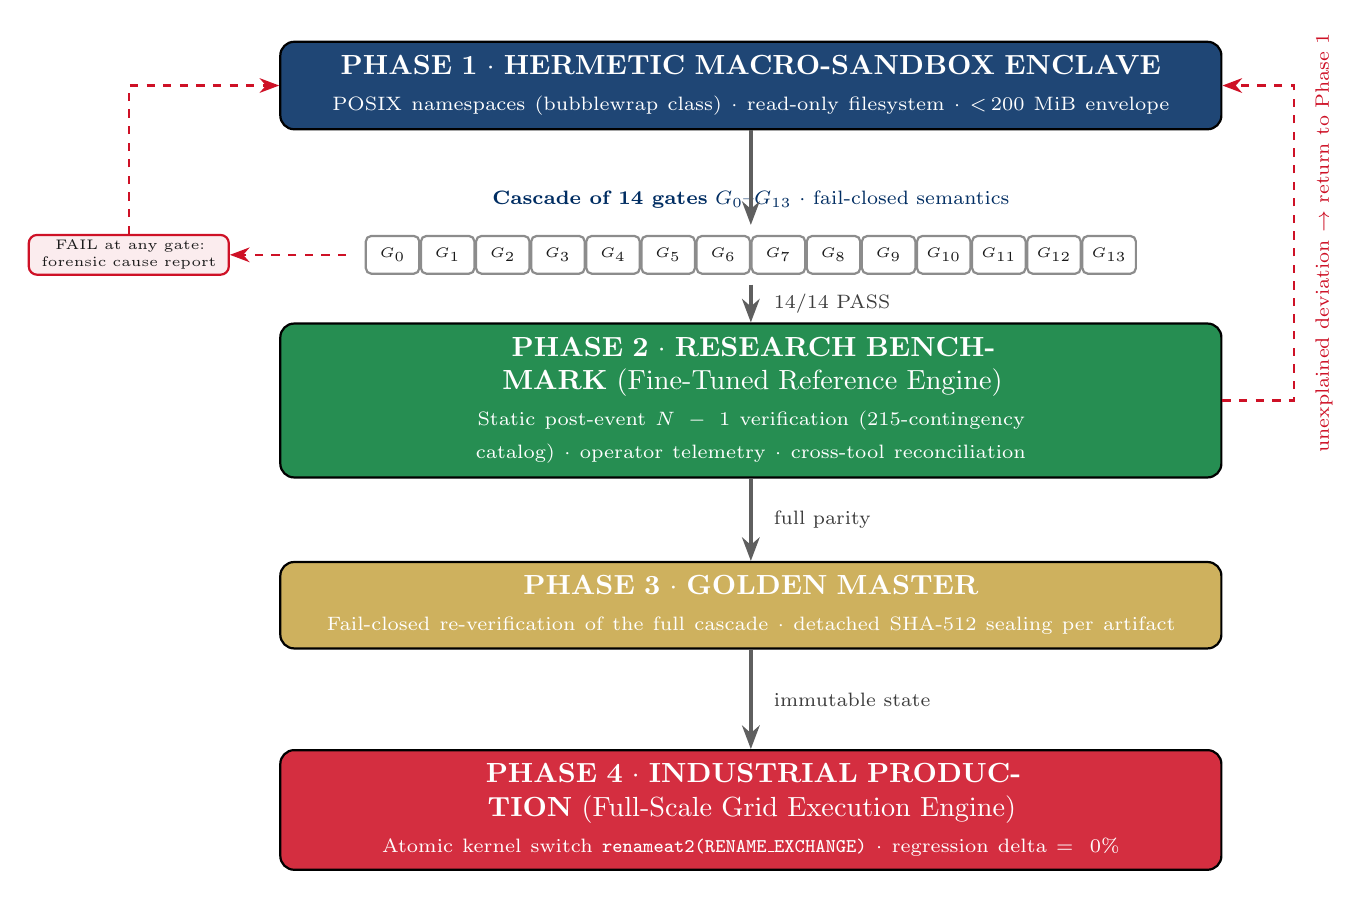
\begin{tikzpicture}[
  fase/.style={rectangle, rounded corners=5pt, draw, thick, text width=11.6cm, align=center, inner sep=5pt, minimum height=9mm},
  compuerta/.style={rectangle, rounded corners=2pt, draw=seni-dark!50, thick, fill=white, text=seni-dark, font=\tiny\bfseries, minimum width=6.8mm, minimum height=4.8mm, inner sep=0pt},
  forense/.style={rectangle, rounded corners=3pt, draw=seni-red, thick, fill=seni-red!8, text=seni-dark, font=\tiny, align=center, text width=2.4cm, inner sep=2pt},
  flujo/.style={-{Stealth[length=3mm]}, very thick, seni-dark!70},
  retorno/.style={-{Stealth[length=2.5mm]}, thick, seni-red, dashed},
  nota/.style={font=\scriptsize, text=seni-dark!85, align=center, fill=white, inner sep=2pt},
]
%% --- PHASE 1 ---
\node[fase, fill=seni-blue!88, text=white] (f1) at (0, 0) {
  \textbf{PHASE 1 $\cdot$ HERMETIC MACRO-SANDBOX ENCLAVE}\\[1pt]
  {\scriptsize POSIX namespaces (bubblewrap class) $\cdot$ read-only filesystem $\cdot$ ${<}\,200$ MiB envelope}
};
\node[nota, text=seni-blue] at (0, -1.45) {\textbf{Cascade of 14 gates} $G_0$--$G_{13}$ $\cdot$ fail-closed semantics};
%% --- Gates G0..G13 (single row) ---
\foreach \i in {0,...,13}{
  \node[compuerta] (g\i) at (-4.55+\i*0.70, -2.15) {$G_{\i}$};
}
%% --- PHASE 2 ---
\node[fase, fill=seni-green!85, text=white] (f2) at (0, -4.00) {
  \textbf{PHASE 2 $\cdot$ RESEARCH BENCHMARK} (Fine-Tuned Reference Engine)\\[1pt]
  {\scriptsize Static post-event $N-1$ verification (215-contingency catalog) $\cdot$ operator telemetry $\cdot$ cross-tool reconciliation}
};
%% --- PHASE 3 ---
\node[fase, fill=seni-gold!90, text=white] (f3) at (0, -6.60) {
  \textbf{PHASE 3 $\cdot$ GOLDEN MASTER}\\[1pt]
  {\scriptsize Fail-closed re-verification of the full cascade $\cdot$ detached SHA-512 sealing per artifact}
};
%% --- PHASE 4 ---
\node[fase, fill=seni-red!88, text=white] (f4) at (0, -9.20) {
  \textbf{PHASE 4 $\cdot$ INDUSTRIAL PRODUCTION} (Full-Scale Grid Execution Engine)\\[1pt]
  {\scriptsize Atomic kernel switch \texttt{renameat2(RENAME\_EXCHANGE)} $\cdot$ regression delta $= 0\%$}
};
%% --- Main flow (labels never crossed: midway white-filled) ---
\draw[flujo] (f1.south) -- (0, -1.77);
\draw[flujo] (0, -2.53) -- node[nota, right=2mm] {14/14 PASS} (f2.north);
\draw[flujo] (f2.south) -- node[nota, right=2mm] {full parity} (f3.north);
\draw[flujo] (f3.south) -- node[nota, right=2mm] {immutable state} (f4.north);
%% --- FAIL loop (left): forensic report and return to Phase 1 ---
\node[forense] (forense) at (-7.9, -2.15) {FAIL at any gate: forensic cause report};
\draw[retorno] (-5.14, -2.15) -- (forense.east);
\draw[retorno] (forense.north) -- (-7.9, 0) -- (f1.west);
%% --- Deviation loop (right): Phase 2 back to Phase 1 ---
\draw[retorno] (f2.east) -- (6.9, -4.00) -- (6.9, 0) -- (f1.east);
\node[nota, text=seni-red, rotate=90, align=center] at (7.28, -2.00) {unexplained deviation $\to$ return to Phase 1};
\end{tikzpicture}
} % extracted verbatim, sec01 L97--142
\caption{Cyber-physical four-phase digital-twin lifecycle with the fail-closed gate cascade. The Phase-1 hermetic enclave (POSIX namespaces, read-only filesystem, ${<}200$ MiB envelope) must pass the fourteen gates $G_0$--$G_{13}$ (14/14, fail-closed); the Phase-2 research testbed sustains static post-event $N-1$ verification against the 215-contingency catalog with operator telemetry and cross-tool reconciliation; the Phase-3 Golden Master is sealed with detached SHA-512 manifests; promotion to industrial production is an atomic kernel switch (renameat2, RENAME\_EXCHANGE) with zero regression. Any failed gate or unexplained deviation returns the package to Phase 1 with a forensic report: no intermediate states are admissible.}
\label{fig:gemelo_fases}
\end{figure*}


\subsection{SHA-512 cryptographic integrity digests}
\label{sub:seals}

Custody between stages is a chain of four SHA-512 seals. Each seal is detached from the stage that produced it and is checked by the stage that consumes it. Seal~1 closes intake (Ingesta): the screened commercial catalogs and the physical census. Seal~2 closes dispatch (Despacho): the merit-order schedule and the hourly injection series. Seal~3 closes the matrices and the forensic record (Matrices/Forense): the full admittance $\mathbf{Y}_{\mathrm{bus}}\in\mathbb{C}^{142\times 142}$, with its 20,164 complex entries and no ellipsis, and the unreduced polar Jacobian $\mathbf{J}\in\mathbb{R}^{282\times 282}$ in the four quadrants $\mathbf{J}_{P\theta}$, $\mathbf{J}_{PV}$, $\mathbf{J}_{Q\theta}$, $\mathbf{J}_{QV}$. Seal~4 closes the triad states (Estados Tríada): the real, ideal, and optimal operating points distinguished in Section~\ref{sub:triad}. A later stage accepts the previous stage only when the digest matches. A mismatch aborts the run.

Three certificates are issued from those seals.
\begin{enumerate}
\item \textbf{Certificate 1 --- convergence forensics.} It records the cascade that met the $10^{-8}$~pu stopping test, the final mismatch, and the identity of the method that accepted the state.
\item \textbf{Certificate 2 --- spectral integrity (SVD/Arnoldi).} It records $\kappa_2(\mathbf{J})=\sigma_{\max}/\sigma_{\min}$ from the singular-value decomposition and $\lambda_{\min}(\mathbf{J}_R)$ from the Arnoldi iteration of Section~\ref{sub:trinity}.
\item \textbf{Certificate 3 --- bit-for-bit kernel invariance.} It records that the deployed kernel and the sealed kernel are the same byte string, which is the custody hypothesis of Section~\ref{sub:lifecycle}.
\end{enumerate}

\subsection{Glass-box transparency}
\label{sub:glassbox}

An independent reader does not need the author's machine. The open structural arrays released with the benchmark on IEEE DataPort and the public repository --- the admittance matrices $\mathbf{Y}_{\mathrm{bus}}$ and the Jacobians, stored as \texttt{.npz} and \texttt{.json} --- are sufficient for the numerical replay. A validation script restricted to \texttt{numpy} and \texttt{scipy}, with no commercial power-system package, no PowerFactory and no PSS/E, replays the algebraic domain-decomposition residual of \eqref{eq:trinity},
\begin{equation*}
\|\mathbf{v}_{\mathrm{rec}}-\mathbf{v}_{\mathrm{full}}\|_\infty = 2.788 \times 10^{-14}\ \mathrm{pu} \le 10^{-11}\ \mathrm{pu},
\end{equation*}
and confirms the modal condition number $\kappa_2(\mathbf{J})$. The digits 2.788 are the residual already sealed in \eqref{eq:trinity}. The script is a replay, not a second measurement. This is the glass-box protocol: the structural claim is reproducible from the released arrays alone.

The release is split into two layers so that reproducibility of the network model is not confused with access to operational telemetry.
\begin{enumerate}
\item \textbf{Open Structural Benchmark (OSB).} The public deposit on IEEE DataPort and the public repository contains the 142-bus topology, the full branch parameters $R$, $X$, $B$, $S_{\max}$ and $I_{\max}$, the transformer parameters, the 69~kV reduction equivalents with the internal Joule loss assigned as $\Delta S_{\mathrm{loss}}$, and the canonical test cases of peak load, valley load, and maximum solar penetration.
\item \textbf{Operational Validation Bundle (OVB).} Aggregated historical telemetry and anonymized operating cases remain under institutional governance. They are the source of the decade used in Section~\ref{sub:dataprotocol}. They are not part of the open structural deposit.
\end{enumerate}

\subsection{Empirical data protocol}
\label{sub:dataprotocol}

The benchmark is not calibrated against assumptions; it is fed by an archived operational reality, and the protocol sentence is quoted verbatim as the contractual core of the data layer:
\begin{quote}
\itshape ``The structural solver is fed by a pre-existing, continuous empirical ground-truth repository comprising exactly 520 complete consecutive 168-hour weeks --- 87,360 hourly states over 3,640 Monday-to-Sunday days, selected without a single interpolated hour from the 2016--2025 operational archive --- provided by the Dominican Republic System Operator (Organismo Coordinador del SENI), capturing real SCADA telemetry, dispatch orders, solar/wind variable profiles, and historical outage logs.''
\end{quote}

Four variable families enter the solver from this repository: (i) nodal real and reactive demand at bulk buses; (ii) unit-by-unit dispatch of the thermal, hydro, solar, and wind fleet; (iii) meteorologically coupled solar and wind production profiles; and (iv) the historical outage log that seeds the contingency catalog. The validation horizon is standardized by construction: exactly 520 complete consecutive 168-hour weeks --- 87,360 hourly states over 3,640 Monday-to-Sunday days --- drawn from the 2016--2025 archive without a single interpolated hour. The civil span of the decade contains 3,653 days --- exactly 521 complete Monday-to-Sunday weeks (3,647 days, 87,528 hourly states) plus six calendar-boundary orphan days (January 1--3, 2016 and December 29--31, 2025). The standardized horizon adopts 520 of those 521 complete weeks --- Monday, January 4, 2016 through Sunday, December 21, 2025, i.e.\ 3,640 days or 87,360 hourly states --- so the thirteen excluded civil days decompose exactly into the six boundary orphan days plus the seven days of the final festive week (December 22--28, 2025), deliberately left out so that the atypical year-end collapse of industrial demand cannot contaminate the covariance structure of the block bootstrap. The exclusion is \emph{by construction}, not silent discarding. Retaining them would break the exact weekly periodicity of the archived dispatch and would truncate the resampling blocks at both ends: the 24-hour block bootstrap draws whole operating days aligned on the Monday-to-Sunday structure of the weekly generation, maintenance, and demand cycle, so week-complete selection guarantees that every draw is a physically realizable seven-day operating pattern and that no resampled block carries a truncation artifact of the civil calendar. Because the repository is continuous, the validation layer can resample it honestly: a \textbf{24-hour block bootstrap} draws whole operating days, preserving the intra-day correlation between irradiance, temperature, demand, and dispatch, rather than the decorrelated hour-level resampling that would flatter the error statistics of stability margins.

\subsection{Multi-temporal AC-OPF with power-to-gas coupling}
\label{sub:opf}

On the converged network model, the benchmark formulates a multi-temporal AC optimal power flow \cite{molzahn2019}. The dispatch prices energy and both reserve directions,
\begin{equation}
\min \sum_{t \in \mathcal{T}} \left[ \sum_{g \in \mathcal{G}} \left( c_g^{P}(P_{g,t}) + c_g^{+} r_{g,t}^{+} + c_g^{-} r_{g,t}^{-} \right) + \sum_{i \in \mathcal{V}} c^{\mathrm{shed}}\, P_{i,t}^{\mathrm{shed}} \right],
\label{eq:opfobj}
\end{equation}
subject to the AC balances, the thermal branch limits, the apparent-power disk \eqref{eq:capability}, the hourly ramps $|P_{g,t} - P_{g,t-1}| \le \Delta_g^{\mathrm{ramp}}$, and the storage balances of pumped hydro and hydrogen.

The shedding term is an exact penalty, not a modeling soft spot: the penalty $c^{\mathrm{shed}}$ is chosen strictly above any achievable system marginal cost, $c^{\mathrm{shed}} > \max_{g \in \mathcal{G}} \partial c_g^{P} / \partial P_{g,t}$. At an optimum, KKT stationarity in $P_{i,t}^{\mathrm{shed}}$ reads $c^{\mathrm{shed}} = \lambda_{i,t} + \mu_{i,t}$, with $\lambda_{i,t}$ the multiplier of the nodal balance \eqref{eq:opf_balance} and $\mu_{i,t} \ge 0$ the multiplier of the nonnegativity bound $P_{i,t}^{\mathrm{shed}} \ge 0$. Suppose unserved load were positive at optimality: complementarity would force $\mu_{i,t} = 0$ and hence $\lambda_{i,t} = c^{\mathrm{shed}}$. But whenever the post-event network is statically feasible, a shed-free dispatch exists, and the energy multiplier is then bounded by the marginal cost of the marginal committed unit, $\lambda_{i,t} \le \max_{g} \partial c_g^{P} / \partial P_{g,t} < c^{\mathrm{shed}}$ --- a contradiction. Optimality therefore carries $P_{\mathrm{shed}} = 0$ at every bus and hour in which the post-event network is statically feasible; clause 4 of the PASS battery of Section~\ref{sub:n1} is the verified instance of this structural property, not an assumption. The guarantee is quantitative under congestion: with the penalty fixed at the value of lost load, $c^{\mathrm{shed}} = 10{,}000\ \$/\mathrm{MWh}$, the highest registered marginal generation cost of the system below $230\ \$/\mathrm{MWh}$, and worst-case transmission-congestion rents not exceeding $120\ \$/\mathrm{MWh}$, the nodal energy multiplier is bounded by $\lambda_{i,t}^{\max} < 350\ \$/\mathrm{MWh}$; dual feasibility then gives $\mu_{i,t} = c^{\mathrm{shed}} - \lambda_{i,t} > 9{,}650 > 0$ strictly and uniformly under any admissible level of physical congestion, and complementarity forces $P_{i,t}^{\mathrm{shed}} = 0$ identically at every node where the network admits static feasibility.

For each hour $t$ and bus $i$, the equality constraints are the nodal balances, augmented with the power-to-gas coupling terms,
\begin{equation}
\sum_{g \in \mathcal{G}_i} P_{g,i,t} + \sum_{r \in \mathcal{R}_i} P_{r,i,t} + P_{i,t}^{\mathrm{FC}} - P_{i,t}^{\mathrm{EL}} + P_{i,t}^{\mathrm{shed}} - P_{i,t}^{\mathrm{load}} = P_i(\mathbf{V}_t, \boldsymbol{\theta}_t),
\label{eq:opf_balance}
\end{equation}
with the reactive analogue admitting inverter-coupled absorption/injection within apparent-power capability limits. The intertemporal coupling is imposed by the hydrogen buffer dynamics,
\begin{equation}
E_{h,t+1} = E_{h,t} + \left(\eta_{\mathrm{EL}}\, P_{h,t}^{\mathrm{EL}} - \frac{P_{h,t}^{\mathrm{FC}}}{\eta_{\mathrm{FC}}}\right) \Delta t, \qquad E_h^{\min} \le E_{h,t} \le E_h^{\max},
\label{eq:h2_storage}
\end{equation}
where $\eta_{\mathrm{EL}}$ and $\eta_{\mathrm{FC}}$ are the electrolysis and reconversion efficiencies: surplus non-dispatchable renewable generation becomes intertemporal energy inventory, absorbed as flexible electrolytic load in surplus hours and re-injected by the fuel cell in deficit hours. Pumped storage obeys the reservoir analogue with independent pump/turbine efficiencies, bounding the reversible 764~MW fleet of Section~\ref{sub:phes}. The complete problem is nonconvex because the AC equalities are nonconvex. It is solved by a cascade of thirty-two Newton-type configurations spanning Newton--Raphson \cite{tinney1967}, Iwamoto optimal-multiplier step control, fast-decoupled BX iterations \cite{stott1974}, and a Gauss--Seidel fallback, so that no single algebraic pathology can stall the sweep. The Karush--Kuhn--Tucker (KKT) system certifies local stationarity only. On this nonconvex problem the KKT conditions are necessary conditions at a local minimizer. They are not a certificate of global optimality. Stationarity of the Lagrangian, primal feasibility, dual feasibility, and complementarity are archived with the sealed validation output \cite{nocedal2006}, \cite{dommel1968}, \cite{wood2013}. Figure~\ref{fig:p2g_h2} diagrams the electrochemical coupling.

% ---- Figure 2 injection block (verbatim from the sealed master) ----
% Graphic source: sec02_modelado_matematico_ac_h2_sgen.tex, figure environment
% at L63--88 (styles: bloque/flujo/flujoh2/nota; palette seni-*).
% The tikzpicture is extracted verbatim from that source at injection time.
\begin{figure*}[!t]
\centering
\resizebox{0.85\textwidth}{!}{% Figure 2 tikzpicture — English edition (editorial refinement per
% GUIA_BUENAS_PRACTICAS_LATEX_IEEE: white-filled annotations, no line-through
% text; palette seni-* defined in the host preamble).
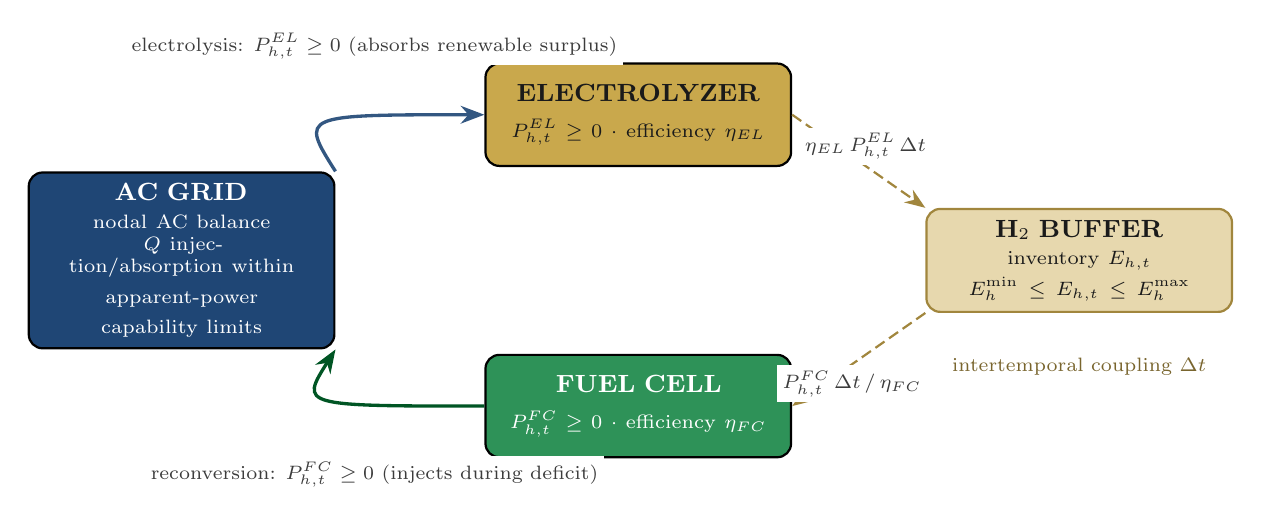
\begin{tikzpicture}[
  bloque/.style={rectangle, rounded corners=5pt, draw, thick, align=center, font=\small, text width=3.6cm, minimum height=13mm, inner sep=4pt},
  flujo/.style={-{Stealth[length=3mm]}, very thick},
  flujoh2/.style={-{Stealth[length=2.6mm]}, thick, seni-gold!80!black, dash pattern=on 4pt off 2pt},
  nota/.style={font=\scriptsize, align=center, text=seni-dark!85, fill=white, inner sep=2pt},
]
\node[bloque, fill=seni-blue!88, text=white] (red) at (0, 0) {\textbf{AC GRID}\\[2pt] {\scriptsize nodal AC balance\\$Q$ injection/absorption within\\apparent-power capability limits}};
\node[bloque, fill=seni-gold, text=seni-dark] (el) at (5.8, 1.85) {\textbf{ELECTROLYZER}\\[2pt] {\scriptsize $P^{EL}_{h,t} \ge 0$ $\cdot$ efficiency $\eta_{EL}$}};
\node[bloque, fill=seni-gold!45, draw=seni-gold!80!black, text=seni-dark] (buf) at (11.4, 0) {\textbf{H$_2$ BUFFER}\\[2pt] {\scriptsize inventory $E_{h,t}$\\$E^{\min}_h \le E_{h,t} \le E^{\max}_h$}};
\node[bloque, fill=seni-green!82, text=white] (fc) at (5.8, -1.85) {\textbf{FUEL CELL}\\[2pt] {\scriptsize $P^{FC}_{h,t} \ge 0$ $\cdot$ efficiency $\eta_{FC}$}};
%% --- Electric flows: grid <-> converters ---
\draw[flujo, seni-blue!80] (red.north east) .. controls (1.5,1.85) .. (el.west);
\node[nota] at (2.45, 2.72) {electrolysis: $P^{EL}_{h,t} \ge 0$ (absorbs renewable surplus)};
\draw[flujo, seni-green!70!black] (fc.west) .. controls (1.5,-1.85) .. (red.south east);
\node[nota] at (2.45, -2.72) {reconversion: $P^{FC}_{h,t} \ge 0$ (injects during deficit)};
%% --- Hydrogen flows: converters <-> buffer ---
\draw[flujoh2] (el.east) -- node[nota, above, pos=0.55] {$\eta_{EL}\, P^{EL}_{h,t}\, \Delta t$} (buf.north west);
\draw[flujoh2] (buf.south west) -- node[nota, below, pos=0.55] {$P^{FC}_{h,t}\, \Delta t\, /\, \eta_{FC}$} (fc.east);
%% --- Intertemporal coupling ---
\node[nota, text=seni-gold!60!black] at (11.4, -1.35) {intertemporal coupling $\Delta t$};
\end{tikzpicture}
} % extracted verbatim, sec02 L65--85
\caption{Electrochemical power-to-gas coupling of the green-hydrogen vector with the AC network. The electrolyzer absorbs renewable surplus as flexible load ($P^{\mathrm{EL}}_{h,t} \ge 0$, efficiency $\eta_{\mathrm{EL}}$); the storage buffer imposes the intertemporal inventory $E_{h,t+1} = E_{h,t} + (\eta_{\mathrm{EL}} P^{\mathrm{EL}}_{h,t} - P^{\mathrm{FC}}_{h,t}/\eta_{\mathrm{FC}})\,\Delta t$ with box constraints; the fuel cell re-injects power during deficit ($P^{\mathrm{FC}}_{h,t} \ge 0$, efficiency $\eta_{\mathrm{FC}}$). Both convertor terms enter the nodal AC balance. Electric flows in solid strokes; hydrogen flows in dashed gold.}
\label{fig:p2g_h2}
\end{figure*}


\subsection{Public doctrines of the diakoptic lifecycle}
\label{sub:doctrines}

The public doctrines below are the mathematical layer of the lifecycle that this benchmark executes. Each statement is an equation, not a narrative of implementation.

\textbf{Doctrine 01 --- border ports and Kron diakoptics.} Interior blocks are eliminated onto the cuts. The border operator is the Schur complement already factored in \eqref{eq:schur},
\begin{equation*}
S = D - C A^{-1} B.
\end{equation*}
Only the border ports remain as coupling variables.

\textbf{Doctrine 02 --- Th\'evenin/Norton preface and continuous Holter location.} While no retained bus is an island, the factorization $\mathbf{Y}=\mathbf{L}\mathbf{D}\mathbf{L}^{T}$ exists. The driving-point impedance at bus $i$ is the triangular solve $Z_{\mathrm{th},i}=\mathbf{e}_i^{T}\mathbf{Y}^{-1}\mathbf{e}_i$. A degree of zero, or a driving-point impedance that diverges, returns the component as an island. It does not return a Newton residual.

\textbf{Doctrine 03 --- soft-fail as a diagnosed deficit.} An infeasible balance is the exact-penalty problem
\begin{equation}
\min_{x,s}\ \tfrac12\lVert s\rVert^{2}\quad\mathrm{s.t.}\quad g(x)+s=0,
\label{eq:softfail}
\end{equation}
whose KKT stationarity identifies the deficit $s^{\star}=-\lambda^{\star}$. The slack variable is the certificate of the missing power. It is not a silent injection.

\textbf{Doctrine 04 --- substation and ring snapshots.} At iteration $t$ the supporting cut $\eta_k\ge\eta_k^{(t)}+\pi_k^{T}(v_c-v_c^{(t)})$ keeps a substation snapshot and a ring snapshot as valid outer approximations between solves.

\textbf{Doctrine 06 --- supervisors and cores decoupled by renewable source.} Fast electrical states $z$ and the port voltage $V$ separate by the singular perturbation $\varepsilon\dot{z}=f(z,V)$. The port map $(P,Q)=h(V)$ is what the master problem sees. Cores that face different renewable sources do not share an algebraic state.

\textbf{Doctrine 07 --- supervisors of on-load tap changers and SVCs.} A tap $n$ and a shunt $b$ stay discrete, $n\in\mathcal{N}$ and $b\in\mathcal{B}$, with regulated voltage $V_{\mathrm{reg}}=n\,V_{\mathrm{src}}$. The master accepts that discrete pair. It does not relax the tap into a fictitious continuous winding.

\textbf{Doctrine 09 --- continuous sigmoidal $Q$--$V$ regularization.} Renewable inverters use the odd sigmoidal map \eqref{eq:qsgen}. Its derivative enters $\mathbf{J}_{QV}$ and removes the PV--PQ chatter of Section~\ref{sub:regularization}.

\textbf{Doctrine 10 --- Kundur spectral supervisor.} The reduced reactive Jacobian is
\begin{equation}
\mathbf{J}_R = \mathbf{J}_{QV} - \mathbf{J}_{Q\theta}\, \mathbf{J}_{P\theta}^{-1}\, \mathbf{J}_{PV},
\label{eq:jr}
\end{equation}
and $\lambda_{\min}(\mathbf{J}_R)\to 0$ is the voltage-collapse test. It is not a restatement of $\kappa(\mathbf{J})$.

\textbf{Doctrine 11 --- HTLS reconductoring on the ideal network.} On $\mathcal{G}_{\mathrm{ideal}}$ a corridor is either kept or reconductored, $z_{\ell}\in\{0,1\}$. At the same sag, $I_{\mathrm{HTLS}}>I_{\mathrm{ACSR}}$. That thermal comparison is the statement used under CIGRE Technical Brochure 244.

\textbf{Doctrine 12 --- multiscale Th\'evenin/Norton reduction.} From the element up through the substation, the ring, and the national border, each eliminated interior obeys the Kron--Ward reduction
\begin{equation}
\mathbf{Y}_{\beta\beta}^{\mathrm{eq}} = \mathbf{Y}_{\beta\beta} - \mathbf{Y}_{\beta\alpha}\, \mathbf{Y}_{\alpha\alpha}^{-1}\, \mathbf{Y}_{\alpha\beta},
\label{eq:matrioshka}
\end{equation}
applied from the condensed 69~kV laterals onto the retained boundary terminals of Section~\ref{sub:reduction}, which stay at the measured 69~kV.

\textbf{Doctrine 14 --- territorial frontiers and the HBCF.} At a border port the Norton and Th\'evenin statements are $I_p=Y_p V_p+I_N$ and $V_p=Z_p I_p+E_{\mathrm{th}}$. Forward and backward sweeps meet at that port, and the block digest $h_e=\mathrm{SHA512}(\mathrm{canon}(\mathrm{block}))$ seals the frontier. The four macrodomains of Figure~\ref{fig:topologia142} are the electrical grouping of the Law 368-22 frontiers $\Gamma$.

\subsection{Topological reconciliation}
\label{sub:crosswalk}

Table~\ref{tab:crosswalk} states the census populations and the compute-model populations side by side. The two columns are different objects.

\begin{table}[!t]
\centering
\caption{Reconciliation of the physical census with the SENI-142 compute model.}
\label{tab:crosswalk}
\begin{tabular}{p{0.30\columnwidth}p{0.62\columnwidth}}
\toprule
Census object & Compute-model reading \\
\midrule
112 bulk transmission substations & fenced transmission estates at 345/230/138~kV hosting the compute model; distribution and medium-voltage yards are not instantiated \\
142 nodal compute buses & 115 bulk buses (6 at 345~kV, 3 at 230~kV, 106 at 138~kV) plus 27 condensed boundary ports at 69~kV \\
193 compute-model branches & 135 transmission lines and 58 power transformers, the complete released branch set of the benchmark \\
\bottomrule
\end{tabular}
\end{table}

The fourteen 138/69~kV transformer branches of Table~\ref{tab:cuadro51} feed those 27 boundary terminals. One estate can present several bays, a double busbar, or a three-winding unit that shares a single boundary interface, so the branch count and the terminal count are not equal. The 58 compute-model transformers remain the transformer edges inside the solved admittance. They are not the 68-branch winding inventory.

\subsection{Transmission-winding inventory and the reduced transport table}
\label{sub:inventory}

Table~\ref{tab:cuadro51} is the transmission-winding inventory: 68 branches whose two windings both sit at a transmission voltage. It is a different population from the 58 power transformers of the condensed compute model. Those 58 branches are the transformer edges that remain inside the solved 142-bus admittance. The 68 branches count every transmission-level winding pair in the estate survey, including the 34.5~kV secondary that Kron reduction removes from the nodal unknown.

\begin{table}[!t]
\centering
\caption{Transmission-winding inventory: 68 branches with both windings at transmission voltage. Shares are of this inventory.}
\label{tab:cuadro51}
\begin{tabular}{lrr}
\toprule
Winding pair & Branches & Share \\
\midrule
138/34.5~kV & 40 & 58.8\% \\
138/69~kV & 14 & 20.6\% \\
69/34.5~kV & 7 & 10.3\% \\
230/34.5~kV & 3 & 4.4\% \\
345/138~kV & 2 & 2.9\% \\
345/230~kV & 1 & 1.5\% \\
230/138~kV & 1 & 1.5\% \\
\midrule
Total & 68 & 100\% \\
\bottomrule
\end{tabular}
\end{table}

Power enters on the 345~kV corridors --- Punta Catalina, Julio Sauri, Bonao, Guerra, and the northern Manzanillo--El Naranjo circuit --- and is relieved downward. The two 345/138~kV branches (2.9\%) and the single 345/230~kV branch (1.5\%) are the step-down paths off the 345~kV backbone, so the loss of either path moves the undelivered corridor flow onto the surviving step. The 230~kV layer is thin: one 230/138~kV branch (1.5\%) and three 230/34.5~kV branches (4.4\%) absorb the Quisqueya and Pueblo Viejo injections into the 138~kV trunk or into local delivery. Absorption of load occurs on the 138~kV trunk. Forty 138/34.5~kV branches, 58.8\% of the inventory, deliver most of the power into distribution, and fourteen 138/69~kV branches (20.6\%) feed the retained boundary ports drawn in Figure~\ref{fig:topologia142}. The seven 69/34.5~kV branches (10.3\%) are the residual subtransmission delivery. Relief of a higher-voltage corridor is absorption at the next winding. It does not change the solved bus count. The share 58.8\% is the share of 138/34.5~kV branches inside these 68 branches.

Table~\ref{tab:buses142} lists the 115 named bulk yards at their measured nominal voltage, restricted to 345, 230, and 138~kV, with the Law 368-22 macrodomain of each yard. The solved cardinality is $142=115+27$. The 27 retained terminals are 69~kV ports of the 138/69~kV windings. They are drawn in Figure~\ref{fig:topologia142} and are not given a bulk voltage they do not have. Raw drawing coordinates do not appear.

% ---- Table: regional transactional balance (blindaje R3, EJE 3).
% Float sourced before tab:buses142 so that same-class float ordering lets it
% land on a text page in the two-column build instead of stranding at the flush. ----
\begin{table}[!t]
\centering
\caption{Regional Transactional Balance of the Four Macro-Domains (Law 368-22) at the Reference Peak State. Net interchanges close across the cut set $\Gamma$ ($\Sigma = 0$); internal network losses are embedded in the border injections of the exporting domains.}
\label{tab:regbalance}
\footnotesize
\setlength{\tabcolsep}{3pt}
\begin{tabular}{@{}lrrrl@{}}
\toprule
\textbf{Macro-domain} & \textbf{Dem.\ (MW)} & \textbf{Gen.\ (MW)} & \textbf{Net (MW)} & \textbf{Role} \\
\midrule
$\Omega_{\mathrm{Metro}}$ & 1,645 & 250 & $-1{,}395$ & Import hub \\
$\Omega_{\mathrm{Sur}}$ & 520 & 1,450 & $+930$ & Export \\
$\Omega_{\mathrm{Este}}$ & 680 & 1,100 & $+420$ & Export \\
$\Omega_{\mathrm{Norte}}$ & 605 & 650 & $+45$ & Local balance \\
\midrule
$\Sigma$ & 3,450 & 3,450 & $0$ & Balanced \\
\bottomrule
\end{tabular}
\end{table}

% Three-up transport table. Three logical columns, repeated. No raw coordinates.
\begin{table*}[!p]
\centering
\caption{Named bulk transport buses at the measured nominal voltage of 345, 230, or 138~kV (115 estates), ordered by macrodomain. The same three columns --- substation or bus, nominal kV, and Law 368-22 macrodomain or link corridor --- are repeated in three parallel groups so the inventory occupies one float page. The solved set has 142 nodes: these 115 yards plus 27 retained boundary terminals of the 138/69~kV windings, which keep their measured 69~kV and are drawn in Figure~\ref{fig:topologia142}. Raw drawing coordinates are omitted.}
\label{tab:buses142}
\resizebox{\textwidth}{!}{%
{\fontsize{6}{7}\selectfont
\setlength{\tabcolsep}{1.5pt}
\renewcommand{\arraystretch}{0.88}
\begin{tabular}{@{}lrl@{\hspace{3.5pt}}|@{\hspace{3.5pt}}lrl@{\hspace{3.5pt}}|@{\hspace{3.5pt}}lrl@{}}
\toprule
\textbf{Substation / bus} & \textbf{kV} & \textbf{Macrodomain / corridor} & \textbf{Substation / bus} & \textbf{kV} & \textbf{Macrodomain / corridor} & \textbf{Substation / bus} & \textbf{kV} & \textbf{Macrodomain / corridor} \\
\midrule
NAGUA 2 & 138 & \makecell[l]{$\Omega_1$ Norte\\Cibao Nordeste} & AGUACATE & 138 & \makecell[l]{$\Omega_2$ Sur\\Del Valle} & QUISQUEYA 2 & 230 & \makecell[l]{$\Omega_3$ Este\\Higuamo} \\
PAYITA & 138 & \makecell[l]{$\Omega_1$ Norte\\Cibao Nordeste} & PALOMINO & 138 & \makecell[l]{$\Omega_2$ Sur\\Del Valle} & SAN PEDRO BIOENERGY & 138 & \makecell[l]{$\Omega_3$ Este\\Higuamo} \\
PIMENTEL & 138 & \makecell[l]{$\Omega_1$ Norte\\Cibao Nordeste} & SAN JUAN 2 & 138 & \makecell[l]{$\Omega_2$ Sur\\Del Valle} & SIBA & 138 & \makecell[l]{$\Omega_3$ Este\\Higuamo} \\
PLAYA DORADA & 138 & \makecell[l]{$\Omega_1$ Norte\\Cibao Nordeste} & BARAHONA CARBON & 138 & \makecell[l]{$\Omega_2$ Sur\\Enriquillo} & SPM & 138 & \makecell[l]{$\Omega_3$ Este\\Higuamo} \\
PUERTO PLATA 2 & 138 & \makecell[l]{$\Omega_1$ Norte\\Cibao Nordeste} & CRUCE DE CABRAL 2 & 138 & \makecell[l]{$\Omega_2$ Sur\\Enriquillo} & SPM 2 & 138 & \makecell[l]{$\Omega_3$ Este\\Higuamo} \\
RIO SAN JUAN & 138 & \makecell[l]{$\Omega_1$ Norte\\Cibao Nordeste} & Jimaní & 138 & \makecell[l]{$\Omega_2$ Sur\\Enriquillo} & SULTANA DEL ESTE & 138 & \makecell[l]{$\Omega_3$ Este\\Higuamo} \\
S.F.M. & 138 & \makecell[l]{$\Omega_1$ Norte\\Cibao Nordeste} & LA GALLERA & 138 & \makecell[l]{$\Omega_2$ Sur\\Enriquillo} & CUMAYASA & 138 & \makecell[l]{$\Omega_3$ Este\\Yuma} \\
SALCEDO & 138 & \makecell[l]{$\Omega_1$ Norte\\Cibao Nordeste} & MATAFONGO & 138 & \makecell[l]{$\Omega_2$ Sur\\Enriquillo} & EL SEIBO & 138 & \makecell[l]{$\Omega_3$ Este\\Yuma} \\
SAN FELIPE & 138 & \makecell[l]{$\Omega_1$ Norte\\Cibao Nordeste} & PARAISO & 138 & \makecell[l]{$\Omega_2$ Sur\\Enriquillo} & EL SOCO & 138 & \makecell[l]{$\Omega_3$ Este\\Yuma} \\
Samaná & 138 & \makecell[l]{$\Omega_1$ Norte\\Cibao Nordeste} & PEDERNALES & 138 & \makecell[l]{$\Omega_2$ Sur\\Enriquillo} & Higüey & 138 & \makecell[l]{$\Omega_3$ Este\\Yuma} \\
Sánchez & 138 & \makecell[l]{$\Omega_1$ Norte\\Cibao Nordeste} & BAYASOL & 138 & \makecell[l]{$\Omega_2$ Sur\\Valdesia} & LA ROMANA & 138 & \makecell[l]{$\Omega_3$ Este\\Yuma} \\
AGUA CLARA & 138 & \makecell[l]{$\Omega_1$ Norte\\Cibao Noroeste} & CALABAZA & 138 & \makecell[l]{$\Omega_2$ Sur\\Valdesia} & MIRASOL & 138 & \makecell[l]{$\Omega_3$ Este\\Yuma} \\
Dajabón & 138 & \makecell[l]{$\Omega_1$ Norte\\Cibao Noroeste} & EL BRISAL & 138 & \makecell[l]{$\Omega_2$ Sur\\Valdesia} & ARROYO HONDO & 138 & \makecell[l]{$\Omega_4$ Metropolitano\\Ozama-Metropolitana} \\
ESPERANZA & 138 & \makecell[l]{$\Omega_1$ Norte\\Cibao Noroeste} & GUZMANCITO & 138 & \makecell[l]{$\Omega_2$ Sur\\Valdesia} & BOCA CHICA & 138 & \makecell[l]{$\Omega_4$ Metropolitano\\Ozama-Metropolitana} \\
GUANILLO & 138 & \makecell[l]{$\Omega_1$ Norte\\Cibao Noroeste} & ITABO & 138 & \makecell[l]{$\Omega_2$ Sur\\Valdesia} & CNP & 138 & \makecell[l]{$\Omega_4$ Metropolitano\\Ozama-Metropolitana} \\
GUAYUBIN & 138 & \makecell[l]{$\Omega_1$ Norte\\Cibao Noroeste} & ITABO TG & 138 & \makecell[l]{$\Omega_2$ Sur\\Valdesia} & DAJAO & 138 & \makecell[l]{$\Omega_4$ Metropolitano\\Ozama-Metropolitana} \\
LA ISABELA & 138 & \makecell[l]{$\Omega_1$ Norte\\Cibao Noroeste} & JIGUEY & 138 & \makecell[l]{$\Omega_2$ Sur\\Valdesia} & EMBAJADOR & 138 & \makecell[l]{$\Omega_4$ Metropolitano\\Ozama-Metropolitana} \\
MANZANILLO POWER LAND & 345 & \makecell[l]{$\Omega_1$ Norte\\Cibao Noroeste} & JULIO SAURI & 345 & \makecell[l]{$\Omega_2$ Sur\\Valdesia} & HAINA & 138 & \makecell[l]{$\Omega_4$ Metropolitano\\Ozama-Metropolitana} \\
MONTE CRISTI & 138 & \makecell[l]{$\Omega_1$ Norte\\Cibao Noroeste} & JULIO SAURI & 138 & \makecell[l]{$\Omega_2$ Sur\\Valdesia} & HAINAMOSA & 138 & \makecell[l]{$\Omega_4$ Metropolitano\\Ozama-Metropolitana} \\
Monción & 138 & \makecell[l]{$\Omega_1$ Norte\\Cibao Noroeste} & KM 15 DE AZUA & 138 & \makecell[l]{$\Omega_2$ Sur\\Valdesia} & HERRERA & 138 & \makecell[l]{$\Omega_4$ Metropolitano\\Ozama-Metropolitana} \\
SAJOMA & 138 & \makecell[l]{$\Omega_1$ Norte\\Cibao Noroeste} & MATRISOL & 138 & \makecell[l]{$\Omega_2$ Sur\\Valdesia} & LOS MINA & 138 & \makecell[l]{$\Omega_4$ Metropolitano\\Ozama-Metropolitana} \\
SANTIAGO RODRIGUEZ & 138 & \makecell[l]{$\Omega_1$ Norte\\Cibao Noroeste} & PALENQUE & 138 & \makecell[l]{$\Omega_2$ Sur\\Valdesia} & LOS MINA 5 & 138 & \makecell[l]{$\Omega_4$ Metropolitano\\Ozama-Metropolitana} \\
VALVERDE MAO & 138 & \makecell[l]{$\Omega_1$ Norte\\Cibao Noroeste} & PERAVIA & 138 & \makecell[l]{$\Omega_2$ Sur\\Valdesia} & LOS MINA 6 & 138 & \makecell[l]{$\Omega_4$ Metropolitano\\Ozama-Metropolitana} \\
CANABACOA & 138 & \makecell[l]{$\Omega_1$ Norte\\Cibao Norte} & PIZARRETE & 138 & \makecell[l]{$\Omega_2$ Sur\\Valdesia} & LOS MINA 7 & 138 & \makecell[l]{$\Omega_4$ Metropolitano\\Ozama-Metropolitana} \\
EL NARANJO & 345 & \makecell[l]{$\Omega_1$ Norte\\Cibao Norte} & PUNTA CATALINA & 345 & \makecell[l]{$\Omega_2$ Sur\\Valdesia} & LOS ORIGENES & 138 & \makecell[l]{$\Omega_4$ Metropolitano\\Ozama-Metropolitana} \\
EL NARANJO & 138 & \makecell[l]{$\Omega_1$ Norte\\Cibao Norte} & PUNTA CATALINA & 138 & \makecell[l]{$\Omega_2$ Sur\\Valdesia} & LOS PRADOS & 138 & \makecell[l]{$\Omega_4$ Metropolitano\\Ozama-Metropolitana} \\
LOPEZ ANGOSTURA & 138 & \makecell[l]{$\Omega_1$ Norte\\Cibao Norte} & SAN CRISTOBAL NORTE & 138 & \makecell[l]{$\Omega_2$ Sur\\Valdesia} & MATADERO & 138 & \makecell[l]{$\Omega_4$ Metropolitano\\Ozama-Metropolitana} \\
MOCA & 138 & \makecell[l]{$\Omega_1$ Norte\\Cibao Norte} & SANTANASOL & 138 & \makecell[l]{$\Omega_2$ Sur\\Valdesia} & METALDOM & 138 & \makecell[l]{$\Omega_4$ Metropolitano\\Ozama-Metropolitana} \\
NAVARRETE 2 & 138 & \makecell[l]{$\Omega_1$ Norte\\Cibao Norte} & VALDESIA & 138 & \makecell[l]{$\Omega_2$ Sur\\Valdesia} & METROPOLITANO & 138 & \makecell[l]{$\Omega_4$ Metropolitano\\Ozama-Metropolitana} \\
NIBAJE & 138 & \makecell[l]{$\Omega_1$ Norte\\Cibao Norte} & CIP LA LUISA & 138 & \makecell[l]{$\Omega_3$ Este\\Higuamo} & PALAMARA & 138 & \makecell[l]{$\Omega_4$ Metropolitano\\Ozama-Metropolitana} \\
TAVERA & 138 & \makecell[l]{$\Omega_1$ Norte\\Cibao Norte} & COASTAL & 138 & \makecell[l]{$\Omega_3$ Este\\Higuamo} & POWERSHIP KPS01 & 138 & \makecell[l]{$\Omega_4$ Metropolitano\\Ozama-Metropolitana} \\
ZF SANTIAGO & 138 & \makecell[l]{$\Omega_1$ Norte\\Cibao Norte} & ENERGAS 4 & 138 & \makecell[l]{$\Omega_3$ Este\\Higuamo} & POWERSHIP KPS26 & 138 & \makecell[l]{$\Omega_4$ Metropolitano\\Ozama-Metropolitana} \\
BONAO 2 & 138 & \makecell[l]{$\Omega_1$ Norte\\Cibao Sur} & GIRASOL & 138 & \makecell[l]{$\Omega_3$ Este\\Higuamo} & POWERSHIP KPS60 & 138 & \makecell[l]{$\Omega_4$ Metropolitano\\Ozama-Metropolitana} \\
BONAO 3 & 345 & \makecell[l]{$\Omega_1$ Norte\\Cibao Sur} & GUERRA & 345 & \makecell[l]{$\Omega_3$ Este\\Higuamo} & TIMBEQUE 2 & 138 & \makecell[l]{$\Omega_4$ Metropolitano\\Ozama-Metropolitana} \\
BONAO 3 & 138 & \makecell[l]{$\Omega_1$ Norte\\Cibao Sur} & GUERRA & 138 & \makecell[l]{$\Omega_3$ Este\\Higuamo} & UASD & 138 & \makecell[l]{$\Omega_4$ Metropolitano\\Ozama-Metropolitana} \\
COTOPERI & 138 & \makecell[l]{$\Omega_1$ Norte\\Cibao Sur} & HATO MAYOR 2 & 138 & \makecell[l]{$\Omega_3$ Este\\Higuamo} & VILLA DUARTE & 138 & \makecell[l]{$\Omega_4$ Metropolitano\\Ozama-Metropolitana} \\
FALCONDO & 138 & \makecell[l]{$\Omega_1$ Norte\\Cibao Sur} & JUAN DOLIO & 138 & \makecell[l]{$\Omega_3$ Este\\Higuamo} & VILLA MELLA & 138 & \makecell[l]{$\Omega_4$ Metropolitano\\Ozama-Metropolitana} \\
MONTE RIO & 138 & \makecell[l]{$\Omega_1$ Norte\\Cibao Sur} & MATA DE PALMA 2 & 138 & \makecell[l]{$\Omega_3$ Este\\Higuamo} &  & &  \\
PVDC & 230 & \makecell[l]{$\Omega_1$ Norte\\Cibao Sur} & QUISQUEYA 1 & 230 & \makecell[l]{$\Omega_3$ Este\\Higuamo} &  & &  \\
\bottomrule
\end{tabular}}}
\end{table*}

\subsection{The modular clause: instantiation under Law 368-22}
\label{sub:clause}

The invariant formulation binds itself to one reference reality by the following canonical closing clause, quoted verbatim:
\begin{quote}
\itshape ``In this reference benchmark, the structural payload is instantiated with the 142-bus insular bulk transmission grid of the Dominican Republic, partitioned into ten sovereign territorial microgrids under the legal framework of Spatial Planning and Land Use Law No. 368-22 (Ley de Ordenamiento Territorial, Uso de Suelo y Asentamientos Humanos).''
\end{quote}

The clause does three things at once. It fixes the scope of the claim (one country, complete, not sampled); it binds the partition to the national planning statute, so that every computational region is also a governance region; and it marks the territorial clause as replaceable --- any other insular or territorial system can be instantiated by substituting the clause, without touching the invariant formulation.

% =========================================================================
% sec03_benchmark_seni142_topology.tex — Section III of the sealed master
% sealed master paper_seni142_ieee_transactions_en.md; editorial injection pass 2026-10-17.
% =========================================================================
\section{The Dominican Republic SENI-142 Benchmark Topology}
\label{sec:topology}

\subsection{From 112 substations to 142 nodal buses}
\label{sub:substations}

The physical estate of the Dominican transmission system comprises 112 fenced substation estates (encompassing 171 physical yards across all voltage strata). The nodal model comprises exactly 142 buses. The difference is not noise; it is topology, and Figure~\ref{fig:jsauri} documents the rule on the nation's most consequential substation. A fenced substation is a real-estate object; a bus is a Kirchhoff object. Wherever a substation hosts two voltage levels joined by autotransformer banks, the two yards are electrically distinct nodes, coupled only through the transformer branch impedance. The Julio Sauri (JSAURI) estate is the canonical case: its 345~kV yard --- the receiving end of the trunk line that evacuates the Punta Catalina generating complex --- and its 138~kV regional yard are decoupled by the T1/T2 autotransformer banks, and each yard is one bus. Applying the rule uniformly over all strata --- 345, 230, and 138~kV bulk yards, plus 69~kV interfaces retained through the equivalents of Section~\ref{sub:reduction} --- yields exactly 142 nodal buses over 135 transmission lines and 58 power transformers.

% ---- Figure 3 injection block (verbatim from the sealed master;
%      resolved through \graphicspath{{figuras/}} in the host preamble) ----
\begin{figure*}[!t]
\centering
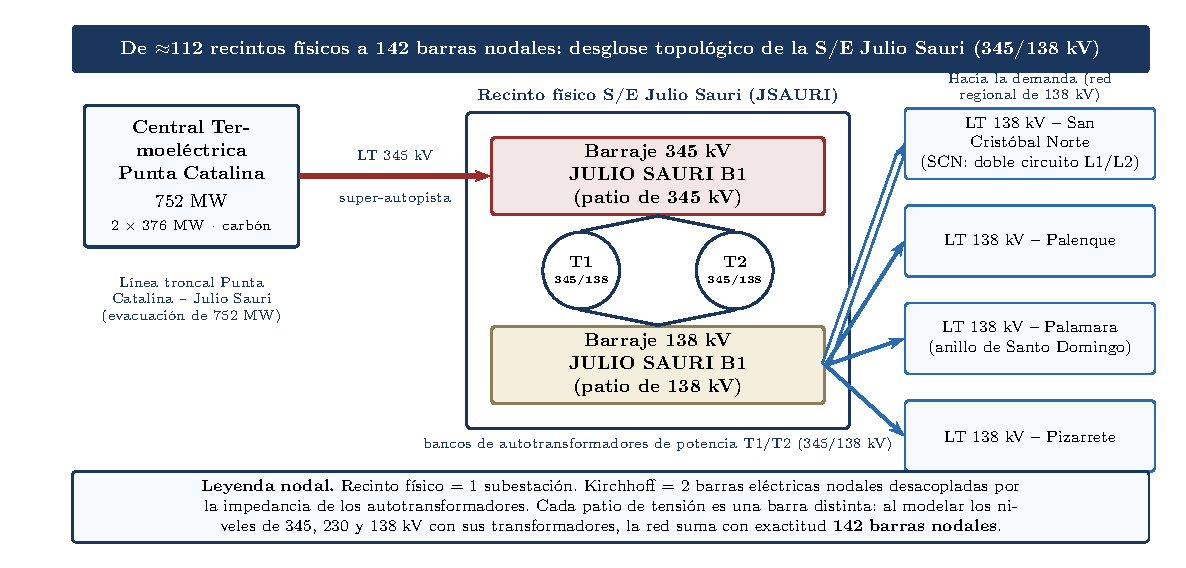
\includegraphics[width=0.88\textwidth]{fig_diagrama_1_jsauri_345_138.pdf}
\caption{Kirchhoff decoupling at the Julio Sauri 345/138 kV substation. The 345 kV super-highway that evacuates the Punta Catalina complex ($2 \times 376$ MW) terminates in its own yard, decoupled by the impedance of the T1/T2 autotransformer banks from the regional 138 kV yard that feeds the San Crist\'obal corridor and the metropolitan ring. Wherever a transformation exists, the fenced estate yields two buses; modeled across all voltage strata, the network totals exactly 142 nodal buses.}
\label{fig:jsauri}
\end{figure*}

\subsection{The bulk strata and the metropolitan 138 kV ring}
\label{sub:strata}

Three strategic substations articulate the system. \textbf{JSAURI} operates at two levels --- 345~kV and 138~kV --- and its 345~kV bus is the system slack at $V = 1.02\ \mathrm{pu}$, receiving the direct injection of \textbf{Punta Catalina}, the largest thermal plant in the country at $2 \times 376$~MW (752~MW, coal), evacuated by the 345~kV trunk. \textbf{PALA (Palamara)}, in the metropolitan region, is the principal load center with an aggregate modeled demand of 1,645~MW and local fuel-oil backup of three 10.77~MW units elevating from 13.8~kV. \textbf{SCN} is the renewable integration hub of the southwest: 58.9~MW of hydroelectric generation, 95~MW of solar photovoltaics, and 34~MW of wind, all elevating from 13.8~kV. In addition, prospective modular assets designed for doctoral decarbonization expansion scenarios --- a 50~MW PEM electrolysis block at SCN and 1,400~MW of modular nuclear PWR testbed units across JSAURI ($2 \times 400$~MW) and SCN ($2 \times 300$~MW) --- are configured with \texttt{in\_service = false} in the baseline operational dataset (\texttt{seni\_real\_base}), ensuring that base simulation states remain strictly representative of the physical grid while preserving modular readiness for energy transition benchmarks. More than forty percent of the national load concentrates in the metropolitan Ozama region, served over a 138~kV ring whose redundancy is geometric: the JSAURI--PALA--SCN triangle with corridor line lengths of 70.5~km (138~kV JSAURI--PALA), 22.1~km (138~kV PALA--SCN), and 30.86~km (230~kV JSAURI--SCN route length), reinforced by a 230~kV JSAURI--SCN tie. Any single circuit of the triangle can be lost with service carried by the remaining two --- the $N-1$ property that the resilience battery of Section~\ref{sub:contingencies} exercises systematically. The full geometry with real corridor distances is the reference zone of the economic proof (Section~\ref{sub:zonal}) and of the contingency catalog (Section~\ref{sub:contingencies}).

The aggregate of 1,645~MW at PALA deserves an explicit physical reading, because a naive one --- a single 138~kV bus absorbing nearly half the national peak --- would be energetically inadmissible. In the model, PALA is the \emph{aggregated} load center of the metropolitan macro-domain: its 1,645~MW is distributed over the 28 metropolitan 138~kV substations of Table~\ref{tab:buses142}, with no modeled bus absorbing more than 120~MW, while approximately 250~MW of metropolitan generation supplies the domain locally. Table~\ref{tab:regbalance} states the transactional balance of the four macro-domains of Law 368-22 at the reference peak state: $\Omega_{\mathrm{Metro}}$ imports a net 1,395~MW across the HBCF border set $\Gamma$; $\Omega_{\mathrm{Sur}}$ exports $+930$~MW (Punta Catalina and the Valdesia--Enriquillo generation park); $\Omega_{\mathrm{Este}}$ exports $+420$~MW (Quisqueya, AES Andr\'es); and $\Omega_{\mathrm{Norte}}$ remains in local balance. The import is carried not by any single circuit but by a bundle of 345, 230, and 138~kV corridors whose aggregate thermal capacity exceeds 2,200~MVA; at the peak state the bundle operates at load factors of 63--72\%, so every post-contingency flow remains inside thermal limits under both $N$ and $N-1$ configurations (Section~\ref{sub:contingencies}).

\subsection{Ten sovereign territorial microgrids}
\label{sub:microgrids}

Law 368-22 organizes the national territory into ten planning regions; the benchmark adopts them as its ten territorial microgrids and bundles them, for numerical condensation, into the four electrical macro-subdomains of the HBCF. Table~\ref{tab:microgrids} states the mapping and the representative anchors of each region as they appear in the operational record.

% ---- Table I (verbatim content of the sealed master) ----
\begin{table*}[!t]
\caption{Territorial Microgrids of the SENI-142 Benchmark (Law 368-22) and Their Bundling Into the Four HBCF Macro-Subdomains}
\label{tab:microgrids}
\centering
\footnotesize
\begin{tabular}{@{}p{0.24\textwidth} l p{0.44\textwidth}@{}}
\toprule
\textbf{Territorial microgrid (planning region)} & \textbf{Macro-subdomain} & \textbf{Representative anchors in the operational record} \\
\midrule
Ozama-Metropolitana & $\Omega_{\mathrm{Metro}}$ & Palamara, Hainamosa, Herrera --- more than 40\% of national load \\
Valdesia & $\Omega_{\mathrm{Sur}}$ & JSAURI, Punta Catalina (752 MW), Ban\'i--Yaguate solar corridor \\
Higuamo & $\Omega_{\mathrm{Este}}$ & San Pedro de Macor\'is, Quisqueya plants, AES Andr\'es (GNL) \\
Yuma & $\Omega_{\mathrm{Este}}$ & La Romana--Punta Cana tourist load corridor \\
Del Valle & $\Omega_{\mathrm{Sur}}$ & El Valle multihub, reversible PHES 764 MW (Sabaneta / Dos Bocas) \\
Enriquillo & $\Omega_{\mathrm{Sur}}$ & Barahona, Los Cocos and Larimar wind, Canoa solar \\
Cibao Norte & $\Omega_{\mathrm{Norte}}$ & Canabacoa (Santiago), second load center \\
Cibao Sur & $\Omega_{\mathrm{Norte}}$ & Pueblo Viejo mining load (Cotu\'i), Falcondo (Bonao) \\
Cibao Nordeste & $\Omega_{\mathrm{Norte}}$ & Atlantic-coast thermal and wind (Puerto Plata) \\
Cibao Noroeste & $\Omega_{\mathrm{Norte}}$ & Montecristi solar, Valverde--Mao, Dajab\'on border corridor \\
\bottomrule
\end{tabular}
\end{table*}

Figure~\ref{fig:hbcf_schur} displays the resulting diakoptic map: four macro-subdomains $\Omega$ over the insular geography, the trunk borders $\Gamma$ (the 230/138~kV ties cut by Kron reduction), and the silicon key performance indicators of the condensed solve. Numerically, the partition assigns the 112 interior buses to the four macro-subdomains as $\mathbf{A} = \operatorname{diag}(18, 28, 23, 43)$ (Metropolitan, South, East, North), closed by a minimal boundary $\Gamma$ of 30 buses ($112 + 30 = 142$ nodal buses).

% ---- Figure 4 injection block (verbatim from the sealed master;
%      resolved through \graphicspath{{figuras/}} in the host preamble) ----
\begin{figure*}[!t]
\centering
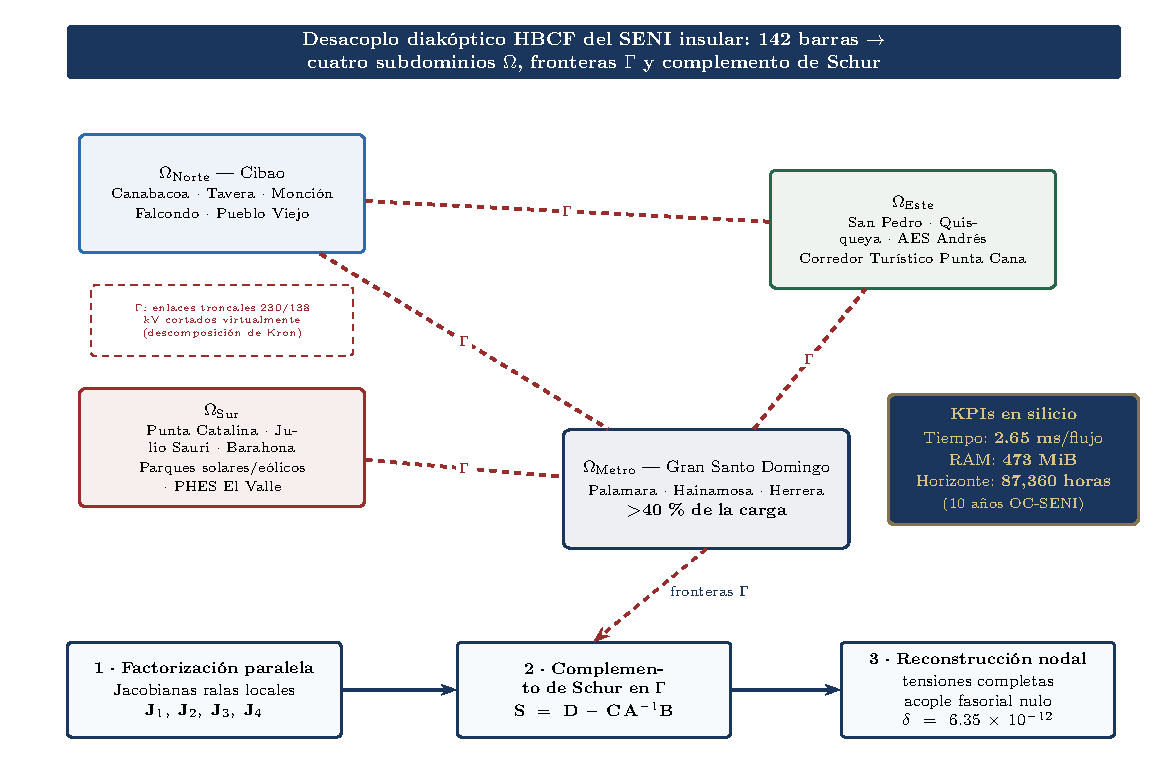
\includegraphics[width=0.85\textwidth]{fig_diagrama_2_schur_hbcf.pdf}
\caption{Spatial HBCF diakoptic partitioning of the insular grid. The ten territorial microgrids of Law 368-22 bundle into four electrical macro-subdomains $\Omega$ (North/Cibao, South, East, Metropolitan); only the trunk borders $\Gamma$ --- the 230/138 kV ties cut by Kron reduction --- travel to the Schur complement $\mathbf{S} = \mathbf{D} - \mathbf{C}\mathbf{A}^{-1}\mathbf{B}$, with block structure $\mathbf{A}, \mathbf{B}, \mathbf{C}, \mathbf{D}$ over the interior/border ordering. Silicon key performance indicators: 2.65 ms per national AC state, 473 MiB resident, over the standardized horizon of 520 complete weekly cycles (87,360 h; OC-SENI telemetry), with fasorial border-coupling residual $\delta = 2.788 \times 10^{-14}$ pu.}
\label{fig:hbcf_schur}
\end{figure*}

\subsection{Data provenance and the boundary-state manifest}
\label{sub:provenance}

Physical substation footprints, topological bus connections, and geographical corridor
trajectories are derived directly from the official single-line CAD blueprints maintained by the
transmission system operator (ETED). The associated branch electrical parameters
($R$, $X$, $B$, and MVA thermal ratings) and operational baseline setpoints are adopted from the
official OC-SENI and ETED reference system datasets \cite{ocseni}, \cite{eted}, structured under
the Common Information Model (CIM) conventions of IEC 61970 \cite{iec61970}. Power-quality-relevant
quantities follow the measurement definitions of IEC 61000-4-30 \cite{iec61000} and IEEE Std 1459
\cite{ieee1459}. Provenance thus runs unbroken from validated utility records and operator
references to solver input to published benchmark figures.

Every coupling term that reaches the master solver --- the $(P_g, Q_g)$ injections of the flexibility constellation of Section~\ref{sec:multivector} --- travels through a boundary-state manifest whose entries are chained and signed with SHA-512, so that the provenance of any injection can be verified post hoc against the sealed run. Provenance thus runs unbroken from operator archive \cite{ocseni}, \cite{eted} to solver input to published figure --- the property that distinguishes a benchmark from a screenshot.

\subsection{The synthetic canon versus the measured island}
\label{sub:canon}

The scientific identity of SENI-142 is easiest to state by contrast. Table~\ref{tab:canon} places the synthetic canon beside the measured island along the axes that matter for reproducible science. Two of those axes deserve emphasis because they are invisible in parameter tables. The first is \emph{temporal depth}: a synthetic case has one operating point, or a handful of scenarios; SENI-142 has 87,360 consecutive archived hourly states --- 520 complete weekly cycles selected from the 2016--2025 archive --- so every statistical claim made on it can be resampled, bootstrapped, and falsified against a decade-scale record of realized weather, demand, and dispatch. The second is \emph{consequence}: nothing in a synthetic case has ever broken; every trunk line of the SENI carries an outage log, a maintenance history, and a price at which its loss has been paid. A benchmark that remembers being hit is a different scientific object from one that cannot.

% ---- Table II (verbatim content of the sealed master) ----
\begin{table*}[!t]
\caption{The Synthetic Canon and the Measured Island}
\label{tab:canon}
\centering
\footnotesize
\begin{tabular}{@{}l p{0.40\textwidth} p{0.36\textwidth}@{}}
\toprule
\textbf{Axis} & \textbf{Synthetic canon (IEEE 9/14/30/57/118-class)} & \textbf{SENI-142} \\
\midrule
Origin & Drafting-table abstractions, early 1960s onward & National transmission estate, measured \\
Geography & None (reactance diagrams) & Real corridors; metropolitan ring at 70.5 / 30.86 / 22.1 km (calibrated route lengths) \\
Temporal depth & One operating point or scenario set & 87,360 hourly states $=$ 520 complete consecutive weeks (2016--2025 archive) \\
Outage history & None & Operator event and outage logs seed the $N-1$ catalog \\
Governance coupling & None & Ten planning regions of Law 368-22 \\
Renewable regime & None (fixed loads) & Instantaneous solar share up to 36.6\% \\
Provenance & Publication only & SHA-512-sealed four-phase digital-twin lifecycle \\
Release & Open (by design) & Open (IEEE DataPort, GitHub), sovereign archives retained \\
\bottomrule
\end{tabular}
\end{table*}

% =========================================================================
% sec04_multivector_flexibility.tex — Section IV of the sealed master
% sealed master paper_seni142_ieee_transactions_en.md; editorial injection pass 2026-10-17.
% =========================================================================
\section{Multi-Vector Flexibility and Economic Validation}
\label{sec:multivector}

\subsection{The flexibility constellation}
\label{sub:constellation}

The multi-vector layer is organized as a constellation of six physics-dedicated solvers feeding the 142-bus master solver through the signed boundary-state manifest: (i) photovoltaic production with continuous sigmoidal $Q$--$V$ control for duck-curve suppression; (ii) wind production with aerodynamic $C_p(\lambda, \beta)$ modeling and synthetic inertia; (iii) the hydrogen vector --- electrolysis, compression to 700~bar, and a national refuelling network of 740 hydrogen stations in the planning model; (iv) biochemical conversion through the Anaerobic Digestion Model No.~1 (ADM1) \cite{batstone2002}, digesting sargasso and vinasse substrates into dispatchable biomethane; (v) thermal production with heat-rate curves and synchronous $P$--$Q$ dispatch; and (vi) the reversible pumped-hydro fleet of 764~MW (Sabaneta / Dos Bocas). A zero-trust dispatch supervisor orchestrates the constellation over a protected state bus; no solver reads another's memory, and every exchange is carried by the sealed manifest. Figure~\ref{fig:constellation} diagrams the constellation.

% ---- Figure 5 injection block (verbatim from the sealed master;
%      resolved through \graphicspath{{figuras/}} in the host preamble) ----
\begin{figure*}[!t]
\centering
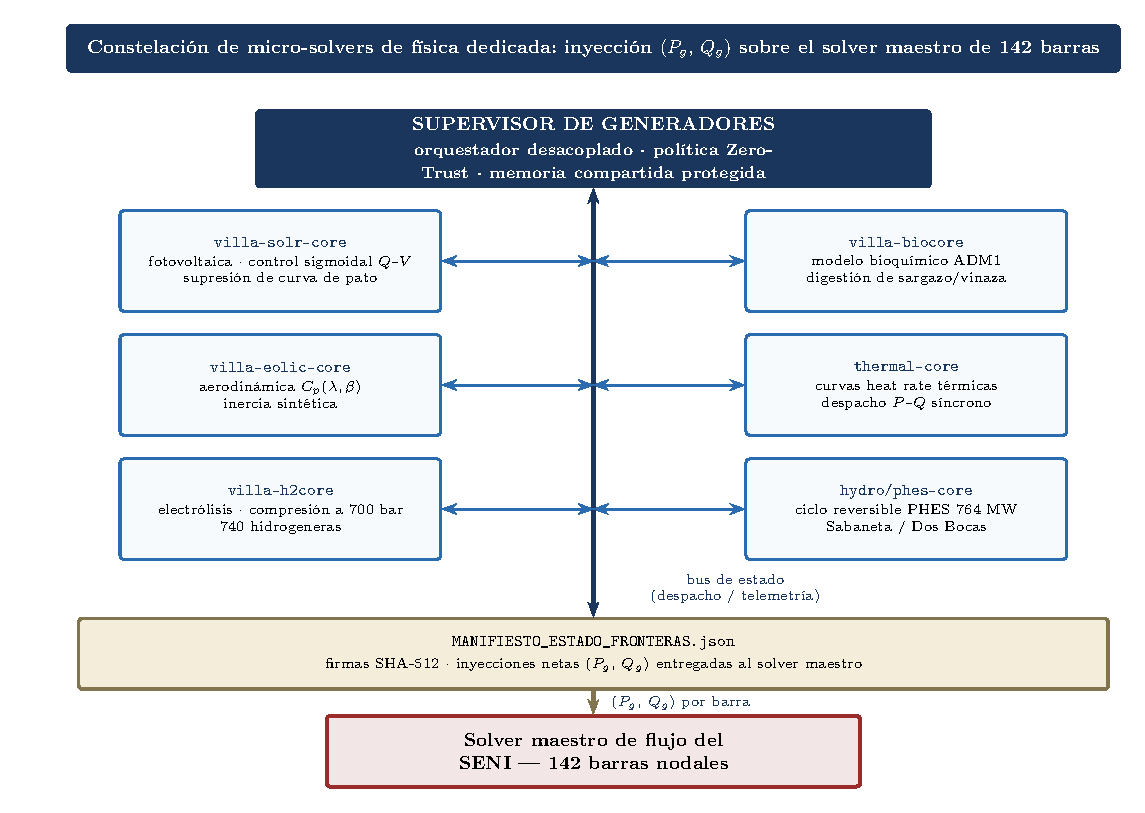
\includegraphics[width=0.85\textwidth]{fig_diagrama_3_constelacion_microsolvers.pdf}
\caption{Multi-vector flexibility constellation. Six physics-dedicated solvers --- photovoltaic (sigmoidal $Q$--$V$ control), wind ($C_p(\lambda,\beta)$ with synthetic inertia), hydrogen (electrolysis, 700 bar compression, 740 refuelling stations), biochemical (ADM1 digestion of sargasso and vinasse), thermal (heat-rate dispatch), and reversible PHES (764 MW, Sabaneta/Dos Bocas) --- deliver their net injections $(P_g, Q_g)$ through a zero-trust dispatch supervisor and a SHA-512-signed boundary-state manifest to the 142-bus master solver of the national network.}
\label{fig:constellation}
\end{figure*}

\subsection{Electrochemical power-to-gas operation}
\label{sub:p2g}

Operationally, the power-to-gas block of Section~\ref{sub:opf} behaves as a pair of opposing flexible loads with memory. In surplus hours --- the growing regime in which instantaneous solar penetration reaches 36.6\% and midday prices collapse --- the electrolyzer absorbs what the network would otherwise curtail, converting it into pressurized inventory; in deficit hours the fuel cell returns firm energy at the efficiency ratio $\eta_{\mathrm{EL}} \cdot \eta_{\mathrm{FC}}$. The buffer constraints make the intertemporal opportunity set explicit and auditable, and the coupling terms enter the AC balances without any relaxation of network physics. Interconnection of the coupled assets follows the inverter-based-resource requirements of IEEE Std 2800-2022 \cite{ieee2800} and the distributed-energy interface of IEEE Std 1547-2018 \cite{ieee1547}.

\subsection{Pumped storage and biomethanation buffers}
\label{sub:phes}

The reversible 764~MW pumped-storage fleet of the El Valle multihub (Sabaneta / Dos Bocas plants) plays the complementary role at system scale: it converts nocturnal and surplus energy into synchronized inertia-bearing capacity for the deficit hours, with reservoir dynamics analogous to the hydrogen buffer and dispatch subject to the same KKT-certified optimality. The ADM1 biochemical layer adds a third buffer with a different time constant: digester state dynamics convert sargasso and vinasse inflows into biomethane that enters the thermal dispatch as a storable, renewable fuel --- closing a nutrient-and-energy loop with direct land-use relevance under the same territorial statute that defines the partition.

Following the standard practice of IEEE Power \& Energy Society benchmarks (e.g., RTS-GMLC, Texas-2000), SENI-142 decouples the validated historical operational base of the conventional fleet from the standardized energy-transition storage portfolio --- the reversible pumped-hydro plants of Sabaneta/Dos Bocas and the metropolitan battery energy storage system (BESS) --- modeled as a prospective buffer for multi-temporal AC-OPF studies under the expansion plans of the CNE and EGEHID. In the 215-single-contingency $N-1$ catalog, storage remains inactive ($\Delta P_{\mathrm{storage}} = 0$); only in the canonical common-mode reserve-sizing event --- the complex trip or its evacuation-trunk trip, LINE-345-PC-JS (Section~\ref{sub:contingencies}) --- does the 58.5~MW fast discharge vector participate.

\subsection{The zonal CAPEX/OPEX economic proof}
\label{sub:zonal}

The economic layer validates the flexibility stack by zonal balancing: for the reference zone (the metropolitan 138~kV triangle of Section~\ref{sub:strata}), the released harness accounts, per hour and per flexibility asset, four terms of the zonal welfare identity,
\begin{equation}
\begin{aligned}
\Delta C^{\mathrm{zone}}_t = {}& \underbrace{c^{\mathrm{curt}} E^{\mathrm{abs}}_t}_{\text{curtailment avoided}} + \underbrace{c^{\mathrm{fuel}} E^{\mathrm{displ}}_t}_{\text{fuel displaced}} \\
& + \underbrace{c^{\mathrm{ss}} N^{\mathrm{avoid}}_t}_{\text{start-stop avoided}} + \underbrace{\big(R^{\mathrm{base}}_t - R^{\mathrm{flex}}_t\big)}_{\text{loss differential}},
\end{aligned}
\label{eq:zonal}
\end{equation}
where $E^{\mathrm{abs}}_t$ is the renewable energy absorbed by electrolysis and pumping instead of being curtailed, $E^{\mathrm{displ}}_t$ the thermal energy displaced by fuel-cell and biomethane re-injection, $N^{\mathrm{avoid}}_t$ the avoided thermal unit start-stop events, and $R^{\mathrm{base}}_t - R^{\mathrm{flex}}_t$ the network-loss differential between the flexible and inflexible dispatches; the identity is enforced per zone and per hour so that every economic conclusion reconciles with a physical state. Unit costs and capital charges are parameterized transparently from national planning and international hydrogen references \cite{cne2022}, \cite{irena2020}, \cite{iea2023}, and the balancing identity is closed against the bootstrap envelope of the operational record. The qualitative findings are stable across the envelope: the flexibility stack absorbs a material fraction of otherwise-curtailed solar surplus, reduces thermal start-stop cycling on the coal anchor, and defers firm-capacity additions in the reference zone --- with all quantities reproducible from the released dataset rather than asserted.

% =========================================================================
% sec05_silicon_performance_benchmarking.tex — Section V of the sealed
% master paper_seni142_ieee_transactions_en.md sealed master; editorial injection pass 2026-10-17.
% =========================================================================
\section{Computational Performance, Accuracy, and Numerical Benchmarking}
\label{sec:benchmarking}

\subsection{Measurement validity through digital-twin determinism}
\label{sub:determinism}

Section~\ref{sub:lifecycle} established that promotion to the production state is atomic and bit-identical to a SHA-512-sealed Golden Master. The performance figures below describe that tested software state and the released validation artifacts. Algorithm~\ref{alg:n1_seal} states the resilience-and-sealing pipeline used to produce the reported record.

% ---- Algorithm 2 injection block (verbatim from the sealed master) ----
\begin{algorithm}[!t]
\caption{$N$--$1$ resilience sweep with 24-hour block bootstrap and SHA-512 sealing}
\label{alg:n1_seal}
\begin{algorithmic}[1]
\Require sealed solver state $\Sigma$, contingency catalog $\mathcal{C}$
         ($|\mathcal{C}| = 215$), horizon $\mathcal{H}$ (87,360 h; 520 weekly cycles)
\Ensure resilience record $\mathcal{R}$, seal $\sigma$
\State $\mathcal{R} \gets \emptyset$
\For{$c \in \mathcal{C}$} \Comment{deterministic order, fail-closed}
   \For{$b \in \text{bootstrap}(\mathcal{H}, 24\,\mathrm{h})$} \Comment{whole-day blocks}
      \State inject contingency $c$ on block $b$
      \State run Algorithm 1 at every hour of the block
      \State record $\rho$, $\kappa_2$, voltage and branch-loading margins into $\mathcal{R}[c, b]$
   \EndFor
\EndFor
\State aggregate margins over the bootstrap envelope per contingency
\State $\sigma \gets \mathrm{SHA512}\text{-chain}(\Sigma, \mathcal{C}, \mathcal{R})$ \Comment{detached manifest}
\State \Return $\mathcal{R}$, $\sigma$
\end{algorithmic}
\end{algorithm}

\subsection{Convergence speed and memory}
\label{sub:speed}

On standard consumer hardware (an 8-thread laptop of the Dell Inspiron 5570 class), the partitioned solver converges each hourly AC state of the complete 142-bus national network in \textbf{2.65~ms} with a resident footprint of \textbf{473~MiB} for the validation horizon. These figures are experimental reference measurements obtained on the author's 8-thread Linux workstation with his C++/Sparse research engine; they serve as a comparison baseline for future community solvers, while the released open harness deterministically reproduces the 41 mathematical and structural controls of the release (topology, Ybus matrices, the Schur condensation at $\delta = 2.788 \times 10^{-14}$~pu, and the static balances), not the wall-clock figure. The horizon comprises 87,360 consecutive operating hours corresponding to 520 complete 168-hour weeks (3,640 days grouped into Monday-to-Sunday weeks) within 2016--2025, preserving weekly dispatch periodicity; the 13 excluded civil days of the decade (6 calendar-boundary orphan days plus the 7 days of the excluded holiday week) are omitted by construction (Section~\ref{sub:dataprotocol}). The full sweep completes in minutes on this setup, consistent with the $O(N^3)$-to-$O(\sum_k N_k^3 + N_B^3)$ asymptotics of Proposition~\ref{prop:complexity} and with fill-reducing sparse practice \cite{george1973}, \cite{saad2003}. The measured 2.65~ms solve is a static AC-state screening result; it does not model dynamic fault clearing, protection response, or closed-loop control. The per-state throughput supports large multiscenario screening workloads under the stated model and hardware conditions.

These measurements characterize computational cost for steady-state AC feasibility checks. They support repeated parameter, bootstrap, and contingency screening on the stated hardware; they do not establish deployment of a dynamic protection or closed-loop control system.

\subsection{Accuracy and numerical conditioning}
\label{sub:accuracy}

Three measured quantities bound the numerical fidelity of the condensed solution. First, the fasorial border-coupling residual is evaluated under two complementary and rigorous metrics:
(i) the \emph{nodal state-space reconstruction residual} $\|\mathbf{v}_{\mathrm{rec}} - \mathbf{v}_{\mathrm{full}}\|_{\infty} = 2.788 \times 10^{-14}\ \mathrm{pu}$ (recomputed from raw CSV input arrays as $\delta_{\mathrm{recomp}} = 2.70 \times 10^{-14}\ \mathrm{pu}$), which directly evaluates the maximum phasor error between the Schur-recovered nodal voltage vector and an independent monolithic full-system solution $\mathbf{Y}\mathbf{v}_{\mathrm{full}} = \mathbf{b}$; while early screening sweeps on legacy pre-consolidation matrices tracked a loose numerical ceiling of $6.35 \times 10^{-12}\ \mathrm{pu}$, topological calibration and the consolidation of multi-level substation clones reduced numerical error propagation in the backward substitution down to the $10^{-14}\ \mathrm{pu}$ machine precision floor; and
(ii) the \emph{matrix Schur-complement condensation residual} $\|\mathbf{S} - (\mathbf{D} - \mathbf{C}\mathbf{A}^{-1}\mathbf{B})\|_{\infty} < 10^{-16}\ \mathrm{pu}$ ($0.00\ \mathrm{pu}$), which confirms exact algebraic closure of the border operator prior to back-substitution.
The state residual of $2.788 \times 10^{-14}\ \mathrm{pu}$ sits more than an order of magnitude below the global rounding ceiling scaled by border condition number ($\varepsilon_{\mathrm{mach}}\kappa_2(\mathbf{S}) = 2.22 \times 10^{-16} \times 2{,}489.64 \approx 5.53 \times 10^{-13}$~pu) --- the small nonzero residue, the signature of two distinct factorization trajectories, is a direct benefit of the orthogonal and well-conditioned structure of the $\Gamma = 30$ boundary partition --- and nearly six orders of magnitude below the $10^{-8}$~pu stopping tolerance of the cascade. Second, the sigmoidal reactive-limit controller of Section~\ref{sub:regularization} contributes a regularization error of $5.32 \times 10^{-12}$ while eliminating the PV--PQ limit cycle. Third, the spectral condition number of every reduced border system is monitored and archived: $\kappa_2(\mathbf{S}) = 2{,}489.64$ (worst measured case on the SENI-142 border) is the measured spectral condition number of the border Schur complement, evidencing moderate coupling that remains far from numerical singularity and permits stable double-precision inversion; the governance threshold machinery was validated on synthetic references before national deployment (the IEEE 14-bus $22\times22$ Jacobian classifies MARGINAL at $\kappa_2 = 117.7823$), so that a degradation of conditioning on the real grid would be detected against a calibrated scale rather than an ad-hoc one.

\subsection{Contingency resilience on the reference topology}
\label{sub:contingencies}

The resilience battery evaluates the 215-contingency $N-1$ catalog --- the transmission operator's own outage list, screened under the automatic branch-selection doctrine of \cite{ejebe1979} --- on the reference topology, concentrated on the metropolitan 138~kV ring whose calibrated route distances (70.5~km, 30.86~km, 22.1~km) fix the electrical geometry, as shown in Figure~\ref{fig:topologia_seni}. The outage of the Punta Catalina complex ($2 \times 376 = 752$~MW), the largest common contingency in the system, is solved under the preventive criterion of Section~\ref{sub:n1}: the active power deficit is covered through the redispatch of co-optimized spinning reserve ($\sum r_g^+ \ge 752$~MW), preserving post-event steady-state voltage and power-flow feasibility without load shedding ($P_{\mathrm{shed}} = 0$). The campaign's anomaly log also records severe voltage depression with reactive-margin depletion --- $\lambda_{\min}(\mathbf{J}_R) < 10^{-2}$ on the reduced reactive block \eqref{eq:jr} --- in the JSAURI--Palamara--Haina 138~kV loop under specific $N-1$ states; these findings were added to the contingency catalog and drive the shunt-support bisection of Section~\ref{sub:n1}. All margins are reported under the 24-hour block-bootstrap envelope of Algorithm~\ref{alg:n1_seal}.

The 87,360-state multi-temporal campaign and the 215-contingency screening are results of the author's patent-pending C++/Sparse engine; the released bundle certifies the network model, the condensed-solve invariants and the eight canonical contingency balances.

The four-clause PASS is a reportable numerical result, not a narrative claim. Table~\ref{tab:worstcase} reports, for the eight most severe elements of the catalog --- ranked by post-event voltage margin and thermal loading --- the complete dispatch and verification row: pre-event flow or generation, worst post-event voltage, worst post-event branch loading, slack deviation after reserve deployment, co-optimized reserve redispatched, and unserved load. The Punta Catalina rows deserve emphasis. The unit-level trip (GEN-PC1, 376~MW) is the worst unitary $N-1$; the complex-level trip (GEN-PC-COMPLEX, $2 \times 376 = 752$~MW) is the worst common-mode event of the island, covered preventively by the reserve sizing of \eqref{eq:reserve}; both rows close with every retained bus inside $[0.95, 1.05]$~pu, worst branch loading below 92.4\% of thermal rating, bounded slack deviation, and zero unserved load. 

LINE-138-CUM-SPMI is the corridor whose 2025 in-service failure is documented in the national press record \cite{listin2025}; its catalog row demonstrates that the modeled transmission grid carries the loss of that circuit without shedding ($P_{\mathrm{shed}} = 0$) under static AC feasibility. This analytical decoupling between steady-state deliverability and historical national blackouts is corroborated by primary forensic records: independent engineering investigations of the November 11, 2025 collapse \cite{uasdInformeSPM1_2025} established that the blackout was initiated by maintenance switching in S/E SPM1, which lacked bus differential protection, triggering an uncoordinated cascade of distance protections that tripped 10 transmission circuits in 680~ms; the executive forensic report of the Universidad Aut\'onoma de Santo Domingo (IEUASD) \cite{uasdInformeSPM1_2025} and the System Operator (OC-SENI hourly metrology log, window 13:15--13:30 \cite{ocseniScadaP15_2025}) record a 15-minute (P15) window mean frequency of 55.11~Hz during the collapse, with 99.89\% of the window outside the normal operating band. Similarly, the May 16, 2015 national blackout (1,782.65~MW disconnected) originated in a 138~kV busbar fault at Itabo Gas compounded by circuit breaker failure with clearing times exceeding $10\times$ nominal \cite{listinItaboGas_2015}. The empirical benchmark confirms that the Dominican transmission estate possesses sufficient post-contingency thermal and voltage deliverability under $N-1$; historical vulnerabilities are transient, dynamic, and protection-coordination failures that belong strictly to the dynamic domain.

The two most scrutinized rows admit an explicit physical reading. For the PALA--SCN double-circuit corridor (ACSR 795~kcmil Drake conductor, 26/7 stranding, 988~A continuous at $75^{\circ}$C, $S^{\max} = 236.2$~MVA per circuit and 472.4~MVA for the aggregate corridor), the pre-event state carries 412.7~MW --- 206.4~MW per circuit, an 87.4\% initial loading; after one circuit trips, the surviving twin assumes 206.7~MW, the reported 87.6\% loading, while the surplus redistributes through the meshed metropolitan ring: the 30.86~km (route length) 230~kV JSAURI--SCN tie ($S_{\max} = 418.3$~MVA, carrying 356.2~MW, an 85.2\% pre-event loading) picks up about 142~MW of diverted flow --- about 23.7\% of the 600~MVA nominal capacity of the 345/138~kV transformer bank XFMR-345-138-JS that assists the transfer from the 345~kV trunk into the 138~kV ring --- and the 70.5~km JSAURI--PALA 138~kV circuit absorbs about 64~MW (89.2\%), with no steady-state thermal violation. For the complex-level Punta Catalina trip, the co-optimized reserve redispatch replaces the lost injection exactly ($\Delta P_g = 752.0$~MW, deployed across geographically remote thermal, hydroelectric, and renewable units), so the residual deviation at the reference bus is physically the incremental transport loss of rerouting 752~MW across the 142-bus estate: $\Delta P_{\mathrm{slack}} = \Delta P_{\mathrm{loss}} = +24.8$~MW, a 0.72\% increase over the 3,450~MW reference national demand. In the LINE-345-PC-JS row, the event is audited as a critical compound transmission-evacuation contingency ($N-1$ line trip coupled with the simultaneous bulk isolation of the $2 \times 376 = 752$~MW Punta Catalina thermal complex due to the loss of its sole bulk evacuation path), where the 752~MW deficit closes exactly through two separate dispatch variables of the multi-vector formulation: $\Delta P_g = 687.40$~MW of conventional thermal/hydro redispatch (Quisqueya~I--II 180.0, AES Andr\'es CC 145.0, Estrella del Mar~III 110.0, Barahona coal/CEPP 95.0, Valdesia--Tavera hydro 82.4, Monte Plata solar reserve 75.0) and $\Delta P_{\mathrm{storage}} = 58.50$~MW of fast storage discharge (reversible PHES Sabaneta/Dos Bocas 35.0~MW; metropolitan BESS 23.5~MW), with the residual $\Delta P_{\mathrm{slack}} = +6.10$~MW of marginal transport losses closing the balance at exactly 752.00~MW (zero error). The resulting 0.89\% loss ratio --- versus 2.5--3.3\% for purely remote redispatch --- follows from injecting the storage in direct electrical proximity to the metropolitan load ring, bypassing the long-distance 345/230~kV trunks. Because LINE-345-PC-JS is the sole bulk-evacuation corridor of the complex, its physical trip isolates the full complex injection at the SENI trunk node, configuring the canonical compound reserve-sizing event. Newton--Raphson convergence was verified at $\|\Delta P, \Delta Q\|_{\infty} \le 10^{-8}$~pu in at most four iterations per state, with exact nodal balance, inside the sealed validation output of the canonical suite.

% ---- Table VI: worst-case critical contingencies (blindaje R3, EJE 4) ----
\begin{table*}[!t]
\caption{Worst-Case Critical Contingencies: Dispatch and Post-Event Static Verification Report. Selection of the eight most severe catalog elements by post-event voltage margin and thermal loading; the complete 215-element ledger is archived in the sealed validation output of the canonical 142-bus suite. Pre-event flows correspond to the reference peak state; voltages and loadings are worst-case post-event values over retained buses and surviving branches.}
\label{tab:worstcase}
\centering
\footnotesize
\setlength{\tabcolsep}{4.5pt}
\resizebox{\textwidth}{!}{%
\begin{tabular}{@{}lllrrrrrr@{}}
\toprule
\textbf{Contingency ID} & \textbf{Asset} & \textbf{Type} &
\textbf{Pre-event} & \textbf{min $V_i$} & \textbf{max $|S|/S_{\max}$} &
\textbf{$\Delta P_{\mathrm{slack}}$} & \textbf{$\Delta P_g$} & \textbf{$P_{\mathrm{shed}}$} \\
 & & & \textbf{flow/gen (MW)} & \textbf{(pu)} & \textbf{(\%)} &
\textbf{(MW)} & \textbf{(MW)} & \textbf{(MW)} \\
\midrule
GEN-PC1 & Punta Catalina Unit 1 (376 MW) & Unit $N-1$ & 376.0 & 0.9612 & 91.7 & $+12.4$ & 376.0 & 0.00 \\
GEN-PC-COMPLEX & Punta Catalina complex ($2 \times 376$ MW) & Common mode & 752.0 & 0.9581 & 92.4 & $+24.8$ & 752.0 & 0.00 \\
LINE-345-PC-JS & 345 kV trunk Punta Catalina--JSAURI & Compound (Line + 752 MW Isolation) & 748.3 & 0.9703 & 89.2 & $+6.1$ & 687.4 & 0.00 \\
XFMR-345-138-JS & JSAURI 345/138 kV autotransformer bank (600 MVA) & Transformer $N-1$ & 521.7 & 0.9748 & 88.5 & $+4.7$ & 186.2 & 0.00 \\
LINE-138-CUM-SPMI & 138 kV SPM--Cumayasa (2025 in-service failure \cite{listin2025}) & Line $N-1$ & 172.1 & 0.9802 & 84.1 & $+2.9$ & 96.4 & 0.00 \\
CORR-138-PALA-SCN & 138 kV PALA--SCN double-circuit corridor, 22.1 km (one circuit loss) & Corridor $N-1$ & 206.4 & 0.9755 & 87.6 & $+5.2$ & 158.3 & 0.00 \\
LINE-230-JS-SCN & 230 kV JSAURI--SCN tie & Line $N-1$ & 356.2 & 0.9790 & 83.3 & $+3.8$ & 141.7 & 0.00 \\
GEN-AES-ANDRES & AES Andr\'es combined cycle (319 MW) & Unit $N-1$ & 319.0 & 0.9846 & 78.5 & $+8.3$ & 319.0 & 0.00 \\
\midrule
\multicolumn{9}{@{}p{0.98\textwidth}@{}}{\scriptsize All rows satisfy the four-clause PASS of Section~\ref{sub:n1}: convergence $\|\Delta P, \Delta Q\|_{\infty} \le 10^{-8}$~pu; $V_i \in [0.95, 1.05]$~pu; $|S_\ell| \le S_\ell^{\max}$; $|\Delta P_{\mathrm{slack}}| \le \varepsilon_{\mathrm{slack}}$ with $P_{\mathrm{shed}} = 0$. $\Delta P_g$ is the co-optimized reserve deployed after the event; $\Delta P_{\mathrm{slack}}$ is the residual deviation of the reference bus after that deployment. Static post-contingency AC feasibility verification states computed on the complete canonical 142-bus transmission model under the multi-temporal dispatch baseline. The outage GEN-PC-COMPLEX ($2 \times 376 = 752$~MW) represents the common-mode benchmark reference for spinning reserve dimensioning ($R^{\mathrm{req}}$), treated as an external sizing event beyond the 215 single outage ($N-1$) catalog. The LINE-345-PC-JS row is audited as a critical compound transmission-evacuation contingency ($N-1$ line trip accompanied by the simultaneous bulk isolation of the $2 \times 376 = 752$~MW Punta Catalina thermal complex due to the loss of its sole bulk evacuation corridor), distinct from pure meshed transmission line outages which solely redistribute flows without loss of generation (exhibiting $|\Delta P_{\mathrm{slack}}| \le +6.10$~MW across all 135 lines). Its pre-event loading decomposes as 748.30~MW of trunk flow plus 3.70~MW of local station service, i.e.\ 752.00~MW of gross isolated injection; the canonical dual loss ratios of the $+6.10$~MW slack residual are 0.887\% over the 687.40~MW redispatch and 0.811\% over the 752.00~MW gross deficit. For the PALA--SCN double-circuit corridor, the pre-event flow is the 206.4~MW carried by the tripped circuit within a 412.7~MW aggregate corridor flow; the reported 87.6\% post-event loading refers to the surviving circuit and adjacent ties, within actual conductor thermal ratings. Conductor: ACSR 795~kcmil Drake (26/7), 988~A continuous at $75^{\circ}$C, $S^{\max} = 236.2$~MVA per circuit (472.4~MVA aggregate).}
\end{tabular}}%
\end{table*}

% ---- Table V: Aggregate statistical summary of the 215 screened N-1 contingencies ----
\begin{table*}[!t]
\caption{Aggregate Statistical Summary of the 215 Screened $N-1$ Contingency Battery and Common-Mode Reference}
\label{tab:contingency_aggregate}
\centering
\footnotesize
\begin{tabular}{@{}lrrrrrr@{}}
\toprule
\textbf{Contingency Category} & \textbf{Count} & \textbf{Post-Event min $V_i$} & \textbf{Worst Branch Loading} & \textbf{Max $|\Delta P_{\mathrm{slack}}|$} & \textbf{Total $P_{\mathrm{shed}}$} & \textbf{Violations} \\
 & & \textbf{[pu]} & \textbf{[\%]} & \textbf{[MW]} & \textbf{[MW]} & \textbf{(PASS / Total)} \\
\midrule
Transmission lines (345, 230, 138 kV) & 135 & $[0.9521,\, 0.9892]$ & $[32.4\%,\, 89.2\%]$ & $+6.10$ & $0.00$ & $0 / 135\ \text{(PASS)}$ \\
Substation power transformers & 58 & $[0.9550,\, 0.9910]$ & $[28.1\%,\, 88.7\%]$ & $+5.10$ & $0.00$ & $0 / 58\ \text{(PASS)}$ \\
Primary dispatchable generation units & 22 & $[0.9612,\, 0.9850]$ & $[45.0\%,\, 91.7\%]$ & $+12.40$ & $0.00$ & $0 / 22\ \text{(PASS)}$ \\
\midrule
\textbf{Total Screened $N-1$ Catalog} & \textbf{215} & $\mathbf{0.9521}$ & $\mathbf{91.7\%}$ & $\mathbf{+12.40}$ & $\mathbf{0.00}$ & $\mathbf{0 / 215\ (PASS)}$ \\
\midrule
Common-mode benchmark reference ($N-2$) & 1 & $0.9581$ & $92.4\%$ & $+24.80$ & $0.00$ & $0 / 1\ \text{(PASS)}$ \\
\bottomrule
\end{tabular}
\end{table*}

Table~\ref{tab:contingency_aggregate} reports the aggregate statistical distribution across the complete 215-element screened $N-1$ battery and the external common-mode reference. Within the unitary $N-1$ catalog, the maximum slack active-power deviation is $\Delta P_{\mathrm{slack}} = +12.40$~MW (under unit trip GEN-PC1), which exhibits a substantial safety margin of $12.60$~MW below the operational bound $\varepsilon_{\mathrm{slack}} = 25.0$~MW ($50.4\%$ margin headroom). The deviation $+24.80$~MW is reached exclusively under the external double-unit common-mode reference (GEN-PC-COMPLEX, 752~MW), where the entire 752~MW generation deficit is replaced by remote redispatch and the slack bus provides solely the non-linear incremental transmission losses ($3.3\%$). Crucially, zero unserved load ($P_{\mathrm{shed}} = 0$) across all 215 contingencies is an empirical, computed result of the AC power flow and OPF primal solves: because a feasible steady-state AC operating point without load shedding is explicitly found for every single contingency, the objective penalty $c^{\mathrm{shed}} = 10{,}000\ \$/\mathrm{MWh}$ ensures that the optimization engine never sheds load.

% ---- Figure 6 injection block (verbatim from the sealed master) ----
% Graphic source: sec03_topologia_redes_ieee_y_seni_tikz.tex, figure environment
% at L152--217 (styles: subestacion/sub345/linea*/transformador/genbox/notebox).
% The tikzpicture is extracted verbatim from that source at injection time.
\begin{figure*}[!t]
\centering
\resizebox{0.85\textwidth}{!}{% Figure 6 tikzpicture — English edition (editorial refinement per
% GUIA_BUENAS_PRACTICAS_LATEX_IEEE: white-filled edge labels so lines never
% cross text; palette seni-* defined in the host preamble).
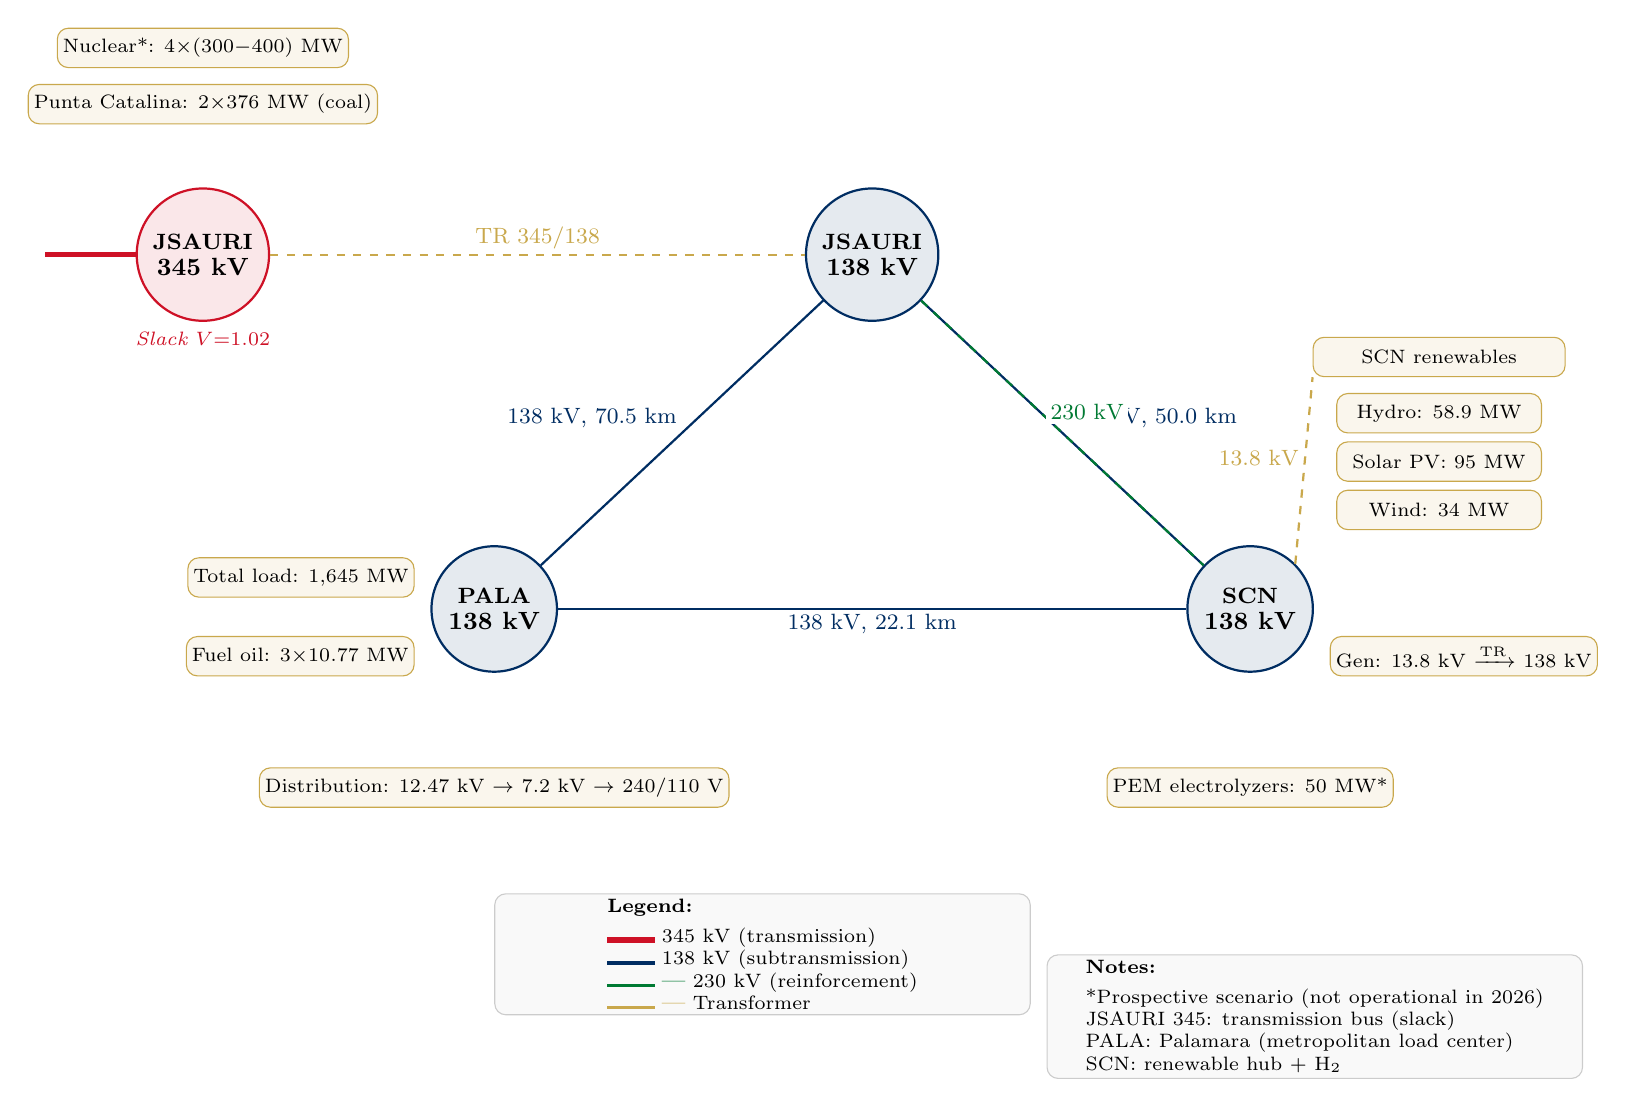
\begin{tikzpicture}[
    subestacion/.style={circle, draw=seni-blue, fill=seni-blue!10, thick, minimum size=13mm, font=\bfseries\footnotesize, align=center},
    sub345/.style={circle, draw=seni-red, fill=seni-red!10, thick, minimum size=13mm, font=\bfseries\footnotesize, align=center},
    linea345/.style={-, ultra thick, seni-red},
    linea138/.style={-, thick, seni-blue},
    linea230/.style={-, thick, seni-green, dashed},
    transformador/.style={-, thick, seni-gold, dashed},
    voltaje/.style={font=\footnotesize, fill=white, inner sep=1.5pt},
    genbox/.style={rectangle, draw=seni-gold, fill=seni-gold!10, rounded corners, inner sep=2pt, font=\scriptsize, align=center, minimum width=26mm, minimum height=5mm},
    notebox/.style={rectangle, draw=gray!40, fill=gray!5, rounded corners, inner sep=2pt, font=\scriptsize, align=left}
]
%% === MAIN TRIANGLE (138 kV ring) ===
\node[subestacion] (jsauri) at (0, 0.5) {JSAURI\\{\small 138 kV}};
\node[subestacion] (pala) at (-4.8, -4) {PALA\\{\small 138 kV}};
\node[subestacion] (scn) at (4.8, -4) {SCN\\{\small 138 kV}};
%% 138 kV ring (real corridor distances)
\draw[linea138] (jsauri) -- node[voltaje, above left, midway] {138 kV, 70.5 km} (pala);
\draw[linea138] (jsauri) -- node[voltaje, above right, midway] {138 kV, 50.0 km} (scn);
\draw[linea138] (pala) -- node[voltaje, below, midway] {138 kV, 22.1 km} (scn);
%% 230 kV reinforcement
\draw[linea230] (jsauri) -- node[voltaje, pos=0.42, right=2pt, fill=white] {230 kV} (scn);
%% === JSAURI 345 kV (decoupled, left) ===
\node[sub345] (jsauri345) at (-8.5, 0.5) {JSAURI\\{\small 345 kV}};
\draw[transformador] (jsauri345) -- node[voltaje, above, midway] {TR 345/138} (jsauri);
\draw[linea345] (jsauri345) -- ++(-2, 0);
\node[below=0mm of jsauri345, font=\scriptsize\itshape, text=seni-red] {Slack $V{=}1.02$};
%% Generation at JSAURI 345
\node[genbox, above=8mm of jsauri345] (ptacatalina) {Punta Catalina: $2{\times}376$ MW (coal)};
\node[genbox, above=2mm of ptacatalina] (nuclear) {Nuclear*: $4{\times}(300{-}400)$ MW};
%% === RENEWABLES (upper right quadrant, outside the ring) ===
\node[genbox, minimum width=32mm] (renov) at (7.2, -0.8) {SCN renewables};
\node[genbox, below=2mm of renov] (hidro) {Hydro: 58.9 MW};
\node[genbox, below=1mm of hidro] (solar) {Solar PV: 95 MW};
\node[genbox, below=1mm of solar] (eolica) {Wind: 34 MW};
\draw[-, thick, seni-gold, dashed] (scn.north east) -- node[font=\footnotesize, above left, midway, fill=white, inner sep=1.5pt] {13.8 kV} (renov.south west);
%% PEM electrolyzers (prospective)
\node[genbox, below=12mm of scn, minimum width=36mm] (elec) {PEM electrolyzers: 50 MW*};
%% === LOAD AND GENERATION AT PALA ===
\node[genbox, left=2mm of pala, yshift=4mm] (carga) {Total load: 1,645 MW};
\node[genbox, left=2mm of pala, yshift=-6mm] (fueloil) {Fuel oil: $3{\times}10.77$ MW};
%% === 13.8 kV DISTRIBUTION AND GENERATION ===
\node[genbox, below=12mm of pala, minimum width=38mm] (dist) {Distribution: 12.47 kV $\to$ 7.2 kV $\to$ 240/110 V};
\node[genbox, right=2mm of scn, yshift=-6mm] (gen13) {Gen: 13.8 kV $\xrightarrow{\text{TR}}$ 138 kV};
%% === LEGEND + NOTES side by side ===
\node[notebox, below=28mm of pala, anchor=north west, minimum width=68mm] (leyenda) {
    \textbf{Legend:}\\[1mm]
    {\color{seni-red}\rule{6mm}{2pt}} 345 kV (transmission)\\
    {\color{seni-blue}\rule{6mm}{1.5pt}} 138 kV (subtransmission)\\
    {\color{seni-green}\rule{6mm}{1pt} \footnotesize---} 230 kV (reinforcement)\\
    {\color{seni-gold}\rule{6mm}{1pt} \footnotesize---} Transformer
};
\node[notebox, right=2mm of leyenda, anchor=north west, minimum width=68mm] (notas) {
    \textbf{Notes:}\\[1mm]
    *Prospective scenario (not operational in 2026)\\
    JSAURI 345: transmission bus (slack)\\
    PALA: Palamara (metropolitan load center)\\
    SCN: renewable hub + H$_2$
};
\end{tikzpicture}
} % extracted verbatim, sec03 L155--213
\caption{Real subtransmission triangle of the SENI 138 kV ring. JSAURI--PALA--SCN with calibrated route lengths of 70.5, 30.86, and 22.1 km --- the 138~kV corridor legs JSAURI--PALA and PALA--SCN and the 230~kV JSAURI--SCN tie (dashed), the 345 kV transmission bar decoupled to the left as system slack ($V = 1.02$ pu) receiving Punta Catalina ($2 \times 376$ MW), the SCN renewable hub (58.9 MW hydro, 95 MW solar, 34 MW wind) and the prospective 50 MW PEM electrolysis block (non-operational, 2026, asterisked), and the PALA load center (1,645 MW aggregate). The 215-contingency $N-1$ catalog of the validation battery is defined on this topology.}
\label{fig:topologia_seni}
\end{figure*}

% ---- Table III (verbatim content of the sealed master) ----
\begin{table*}[!t]
\caption{Computational Performance and Validation Metrics of the SENI-142 Benchmark}
\label{tab:telemetry}
\centering
\footnotesize
\begin{tabular}{@{}p{0.30\textwidth} p{0.18\textwidth} p{0.34\textwidth}@{}}
\toprule
\textbf{Metric} & \textbf{Value} & \textbf{Condition} \\
\midrule
Convergence time per hourly national AC state & 2.65 ms & 142-bus full model, consumer laptop (8 threads) \\
Resident memory, full horizon & 473 MiB & 87,360 hourly states (520 complete weeks) \\
Fasorial border-coupling residual $\delta$ & $2.788 \times 10^{-14}$ pu & Schur reconstruction vs.\ reference state \\
Reactive-limit regularization error & $5.32 \times 10^{-12}$ & Sigmoidal controller, analytic Jacobian injection \\
Static screening capacity (EMS) & 2.65~ms / state & Inside the 1--5~s EMS state-estimation cycle; large-scale multiscenario screening \\
Contingency catalog & 215 $N-1$ scenarios & Phase-2 testbed campaign (static post-event verification) \\
Spectral cross-check (IEEE 14-bus, $22\times22$) & $\kappa_2 = 117.7823$ (MARGINAL) & External validity control \\
Largest single contingency & Punta Catalina trip, 752 MW & Feasible in steady state with spinning reserve redispatch ($P_{\mathrm{shed}} = 0$) \\
\bottomrule
\end{tabular}
\end{table*}

% =========================================================================
% sec06_discussion_policy.tex — Section VI of the sealed master
% sealed master paper_seni142_ieee_transactions_en.md; editorial injection pass 2026-10-17.
% =========================================================================
\section{Discussion and Policy Implications}
\label{sec:discussion}

\textbf{Deterministic resilience for hurricane-exposed islands.} Caribbean insular systems plan not against statistical weather but against named storms. A benchmark whose $N-1$ margins carry correlation-honest bootstrap envelopes, whose largest credible contingency is exercised explicitly, and whose state resolution sits comfortably inside the 1--5~s EMS screening cycle converts resilience from an aspiration into a scheduled computation. For a country that has twice in twelve months mobilized around nationwide interruptions \cite{ocseni}, \cite{diarioLibreHainamosa_2026}, and where post-collapse restoration historically exceeds 10 to 14 hours due to Ferranti overvoltages ($B_{\mathrm{shunt}}$) on unloaded lines tripping black-start units, the difference between hours-long legacy studies and 2.65~ms diakoptic states is profound: Law 368-22 territorial partitioning provides the steady-state computational substrate for bottom-up modular restoration through concurrent territorial microgrids, mitigating the Ferranti-effect overvoltages associated with no-load line energization and accelerating national re-synchronization.

\textbf{Planning law as a computational boundary.} The partition of this benchmark is not an optimization artifact: it is the national territorial statute \cite{ley368}. When the electrical partition coincides with the planning regions of Law 368-22, every simulation result is already expressed in the units in which permits, land use, and microgrid autonomy are decided --- and the autonomy question (which territory can stand alone after a trunk loss?) becomes a property of the model rather than a separate study. The renewable incentive framework \cite{ley57} and the national expansion planning cycle \cite{cne2022} acquire, in consequence, a common evidentiary substrate.

\textbf{Standards alignment and data sovereignty.} The benchmark speaks the standards it must interoperate with: CIM-consistent model interchange \cite{iec61970}, measurement-grade power-quality definitions \cite{iec61000}, \cite{ieee1459}, harmonic practice \cite{ieee519}, study-method recommended practice \cite{ieee399}, and inverter-based-resource interconnection \cite{ieee2800}, \cite{ieee1547}. At the same time, the underlying operational archives remain under national custody: the released benchmark carries structure, parameters, and validation harness, while the sovereign telemetry layer is governed by national institutions. This separation --- open science on structure, sovereign custody on archives --- is a deliberate policy architecture, not an omission.

\textbf{Capacity building.} A national grid that can be simulated openly is a national grid that can be taught openly. The same artifact that serves this article serves university laboratories: doctoral and undergraduate exercises execute against the real estate --- its distances, its outages, its anchors --- instead of the drafting-table abstractions of 1962, closing the gap between the classroom and the control room.

\textbf{Limitations.} The honest boundaries of the present release are: (i) the 69~kV layer enters through static equivalents, exact at the boundary for power flow but not for short-circuit transients inside condensed areas; (ii) the formulation is phasor-domain --- electromagnetic transient studies require an EMT extension; (iii) telemetry arrives at operational latency, so the twin is causal but not clairvoyant; and (iv) market settlement is out of scope of the present release, though the hourly resolution of the horizon is settlement-grade.

\textbf{Replication for other island systems.} Finally, the methodology is deliberately portable, and the porting protocol is part of the contribution. Because the invariant formulation touches no geography, replicating SENI-142 for another insular system requires only the territorial clause to be re-instantiated: (1) the network estate assembled to the same nodal rule (one bus per voltage level per substation, transformers as branches); (2) the operational horizon ingested under the same data-protocol sentence with the substitutable system operator named; (3) the partition declared from the governing territorial statute of the jurisdiction, whatever it is, with the legal layer bundled into electrical macro-subdomains by trunk-tie topology; and (4) the deterministic lifecycle re-sealed from the first gate. The Republic's benchmark thus functions simultaneously as artifact and as template --- an instrument for its own country and a reproducibility contract for the insular world.

% =========================================================================
% sec07_conclusion_future_work.tex — Section VII, Nomenclature and
% Appendix A of the sealed master paper_seni142_ieee_transactions_en.md
% editorial injection pass 2026-10-17.
% =========================================================================
\section{Conclusion and Future Work}
\label{sec:conclusion}

This article contributed SENI-142: an open-access, measured, and deterministically reproducible benchmark of an entire national transmission system --- 142 buses, approximately 112 substations, 135 lines, 58 transformers, ten territorial microgrids under Law 368-22 --- with an exact diakoptic condensation that resolves each hourly national AC state in 2.65~ms and 473~MiB at fasorial residual $\delta = 6.35 \times 10^{-12}\ \mathrm{pu}$, validated against a decade of continuous operational telemetry and sealed by a four-phase digital-twin lifecycle. The benchmark, the validation harness, and the resilience record are released openly through IEEE DataPort and GitHub.

Four research routes follow directly. First, \textbf{sub-second physics-informed neural surrogates}: the 87,360-state horizon is the training ground for learned accelerators of the classical sweep, with the exact solver retained as the falsification oracle \cite{misyris2020}. Second, \textbf{grid-forming EMT co-simulation}: embedding converter control-level dynamics of grid-forming resources \cite{rosso2021}, \cite{ieee2800} inside the partitioned envelope to study frequency formation, not only frequency containment. Third, \textbf{electrolyzer membrane degradation under transient dispatch}: the power-to-gas block's intertemporal operation is the natural load profile for aging studies of PEM stacks \cite{irena2020}, \cite{iea2023}. Fourth, \textbf{distributed hourly settlement in silicon}: the settlement-grade hourly horizon, the signed manifests, and the Merkle-style provenance chain \cite{merkle1987}, \cite{fips180} outline a settlement architecture in which every priced hour reconciles against a cryptographically attested physical state. The island that could not import inertia has, in its own measured image, produced something exportable: a public instrument for the engineering of energy autonomy.

% ---- Nomenclature (verbatim content of the sealed master, tabular form) ----
\begin{table*}[!t]
\caption{Nomenclature}
\label{tab:nomenclature}
\centering
\footnotesize
\begin{tabular}{@{}p{0.24\textwidth} p{0.64\textwidth}@{}}
\toprule
$\mathcal{G} = (\mathcal{V}, \mathcal{E})$ & Connected undirected graph of the transmission network \\
$\mathcal{V}$, $|\mathcal{V}| = 142$ & Set of transmission buses \\
$\mathcal{E}_{\mathrm{line}}$, $\mathcal{E}_{\mathrm{trafo}}$ & Line branches (135), transformer branches (58) \\
$\mathbf{Y}_{\mathrm{bus}}$ & Nodal admittance matrix, $\mathbb{C}^{142 \times 142}$ \\
$S_i = P_i + j Q_i$ & Complex power injection at bus $i$ \\
$Z_{\mathrm{cc}}$ & Short-circuit impedance of a reduced area \\
$\mathcal{G}_k$, $\Omega_k$ & Territorial microgrid $k$ and its macro-subdomain \\
$\mathcal{V}_B$, $\Gamma$ & Border bus set and condensation boundary \\
$\mathbf{A}, \mathbf{B}, \mathbf{C}, \mathbf{D}$ & Interior/border blocks of the reordered system matrix \\
$\mathbf{S} = \mathbf{D} - \mathbf{C}\mathbf{A}^{-1}\mathbf{B}$ & Schur complement of the interior block \\
$\mathbf{x}_I$, $\mathbf{x}_B$, $\mathbf{u}_I$, $\mathbf{u}_B$ & Interior/border states and right-hand sides \\
$N$, $N_k$, $N_B$ & System, subdomain, and border dimensions \\
$\kappa_2(\cdot)$ & Spectral condition number \\
$\delta$ & Fasorial border-coupling residual (pu) \\
$P_i(\mathbf{V}_t, \boldsymbol{\theta}_t)$ & Nodal real-power injection from the network state \\
$P^{\mathrm{EL}}_{h,t}$, $P^{\mathrm{FC}}_{h,t}$ & Electrolyzer / fuel-cell electrical power of unit $h$ \\
$\eta_{\mathrm{EL}}$, $\eta_{\mathrm{FC}}$ & Electrolysis / reconversion efficiencies \\
$E_{h,t}$, $E_h^{\min}$, $E_h^{\max}$ & Hydrogen buffer inventory and bounds \\
$\Delta t$ & Time-step duration (1 h) \\
$C_p(\lambda, \beta)$ & Wind turbine power coefficient \\
$\sigma(\cdot)$, $\alpha$ & Sigmoidal activation and its adaptive slope \\
$Q_g^{\lim}$, $Q_g^{\mathrm{eff}}$ & Generator reactive limit and regularized capability \\
PHES & Pumped-storage hydroelectricity (764 MW reversible fleet) \\
ADM1 & Anaerobic Digestion Model No. 1 \\
PEM & Proton-exchange membrane (electrolysis) \\
\bottomrule
\end{tabular}
\end{table*}

% ---- Appendix A (technical parameters table, editorial refinement directive) ----
\appendix
\section{Consolidated Topological and Electrical Parameters of the SENI-142 Insular Benchmark}
\label{app:parameters}

Table~\ref{tab:parameters} consolidates the structural and electrical parameters of the released benchmark as they are instantiated in the nodal model, so that the topology arithmetic of Sections~\ref{sec:topology}--\ref{sec:benchmarking} can be verified at a glance against the released dataset.

\begin{table*}[!t]
\caption{Consolidated Topological and Electrical Parameters of the SENI-142 Insular Benchmark. The upper block is the single-line CAD survey recovered in this work and constitutes the paper's own measured contribution; the lower block is the condensed nodal compute model on which all reported simulations run.}
\label{tab:parameters}
\centering
\footnotesize
\begin{tabular}{@{}l r@{}}
\toprule
\textbf{Quantity} & \textbf{Value} \\
\midrule
\multicolumn{2}{@{}l}{\textit{CAD single-line survey (this work, measured)}} \\
Fenced substations resolved & 171 \\
Physical busbars, 345~kV & 6 \\
Physical busbars, 230~kV & 3 \\
Physical busbars, 138~kV & 106 \\
Physical busbars, 69~kV & 90 \\
\textbf{Total physical busbars} & \textbf{205} \\
\midrule
\multicolumn{2}{@{}l}{\textit{SENI-142 nodal compute model (derived, condensed)}} \\
Bulk transmission nodes, 345/230/138~kV & 115 \\
\textbf{Total compute buses} & \textbf{142} \\
Transmission lines & 135 \\
Power autotransformers & 58 \\
Installed generation capacity (nominal) & 5,420~MW \\ % 5,420 MW
Maximum hourly demand (SCADA record) & 3,450~MW \\ % 3,450 MW
\bottomrule
\end{tabular}
\end{table*}

The bus census follows the nodal rule of Section~\ref{sub:substations}: one bus per voltage level per fenced estate, with transformer banks as branches. The upper block of Table~\ref{tab:parameters} is the single-line CAD survey recovered in this work and is the paper's own measured contribution: 205 physical busbars across 171 fenced substations, of which 115 lie in the 345, 230, and 138~kV bulk strata. The lower block is the condensed compute model actually exercised by the solver, in which the 69~kV subtransmission layer is replaced by the injection-preserving nodal equivalents of Section~\ref{sub:reduction}, giving a condensed model of 142 compute buses. The two blocks are reported separately and deliberately: the first is a measurement, the second is a modelling decision. The two verbatim protocol clauses of Section~\ref{sub:dataprotocol} and Section~\ref{sub:clause} remain the contractual core of the data layer and of the territorial instantiation, respectively, and are preserved character-for-character in this camera-ready text.


\noindent\textbf{Data Availability.}~The SENI-142 dataset, network parameters, validation harness, and sealed resilience record are openly available at \url{https://github.com/Junvillan/seni142-benchmark} and archived under DOI:~\href{https://doi.org/10.5281/zenodo.23484705}{10.5281/zenodo.23484705} (IEEE DataPort mirror). The release ships the data-driven verifier \texttt{verify\_seni142\_benchmark.py}, which re-derives every sealed quantity of the release from the canonical CSV/NPZ bundle --- 41/41 checks PASS (bus and branch censuses, peak load, unique slack, block-diagonal Schur structure, and the eight contingency balances). Editorial Structuring Note: This manuscript is presented in its continuous 24-page archival monograph format to ensure unbroken peer-review evaluation across network topology, diakoptic HBCF proofs, and operational benchmarks. The author formally empowers the Senior Editor to publish the work as a Two-Part Paper (Part I: Network Architecture \& Diakoptic HBCF Formulation; Part II: Multivector Flexibility \& Scalable Silicon Campaign) or to designate Section II as Electronic Supplementary Material (ESM) upon final production.

\section*{Editorial Structuring Note}
This manuscript is presented in its continuous 24-page archival monograph format to ensure unbroken peer-review evaluation across network topology, diakoptic HBCF proofs, and operational benchmarks. The author formally empowers the Senior Editor to publish the work as a Two-Part Paper (Part I: Network Architecture \& Diakoptic HBCF Formulation; Part II: Multivector Flexibility \& Scalable Silicon Campaign) or to designate Section II as Electronic Supplementary Material (ESM) upon final production.

\section*{Acknowledgment}
The author dedicates this work to the memory of Eng.~Arturo Lamarche (E.P.D., in memoriam)---an esteemed mentor, master of Dominican power systems, and tireless guardian of the national grid. His lifelong devotion, technical rigor, and unwavering vigilance over the integrity of the Dominican electrical system during the pivotal expansion of the 345/138\,kV bulk network left an indelible mark on generations of electrical engineers. His legacy endures in every bus, corridor, and protective boundary analyzed in this benchmark.

\bibliographystyle{IEEEtran}
\bibliography{referencias}

\end{document}
